% !TEX program = xelatex % (can also use "lualatex") 
\documentclass[12pt,a4paper]{report}

% ==========================================
% PACKAGES ESSENTIELS
% ==========================================
% NOTE: inputenc and fontenc are NOT used with XeLaTeX/LuaLaTeX
% fontspec must come before polyglossia
\usepackage{fontspec}
% ---- Main Latin font: Times New Roman ----
% mathpazo is intentionally removed — it overrides setmainfont in XeLaTeX
\setmainfont{Times New Roman}[
    BoldFont       = {Times New Roman Bold},
    ItalicFont     = {Times New Roman Italic},
    BoldItalicFont = {Times New Roman Bold Italic}
]
% ---- Monospaced font that supports Arabic ----
\setmonofont{DejaVu Sans Mono}[Scale=MatchLowercase]   % <-- FIX ADDED HERE
% ---- Arabic font — only active inside \begin{Arabic}...\end{Arabic} ----
\usepackage{polyglossia}
\setmainlanguage{french}
\setotherlanguage[numerals=maghrebi]{arabic}
\newfontfamily\arabicfont[
    Script=Arabic,
    Scale=1.15,
    RightToLeft
]{Amiri}
\usepackage{geometry}
\usepackage{graphicx}
\usepackage{xcolor}
\usepackage{hyperref}
\usepackage{fancyhdr}
\usepackage{titlesec}
\usepackage{float}
\usepackage{microtype}
\usepackage{setspace}
\usepackage{listings}
\usepackage[most]{tcolorbox}
\usepackage{fontawesome5}
\usepackage{booktabs}
\usepackage{array}
\usepackage{colortbl}
\usepackage{mdframed}
\usepackage{enumitem}
\usepackage{tikz}
\usetikzlibrary{shapes, arrows.meta, positioning, calc, decorations.pathreplacing}
\usepackage{pgfplots}
\pgfplotsset{compat=1.18}
\usepackage{multicol}
\usepackage{caption}
\usepackage{subcaption}
\usepackage{amsmath}
\usepackage{amssymb}
\usepackage{soul}
\usepackage{pifont}
\usepackage{tabularx}
\usepackage{adjustbox} % add this to your preamble if not already there

% ==========================================
% PALETTE DE COULEURS - Moroccan Legal RAG
% ==========================================
\definecolor{PrimaryBlue}{RGB}{15, 52, 96}
\definecolor{AccentBlue}{RGB}{52, 120, 246}
\definecolor{LightBlue}{RGB}{235, 243, 255}
\definecolor{DarkGray}{RGB}{45, 45, 55}
\definecolor{MidGray}{RGB}{110, 110, 125}
\definecolor{LightGray}{RGB}{245, 246, 250}
\definecolor{BorderGray}{RGB}{220, 222, 230}
\definecolor{Sandstone}{RGB}{245, 240, 232}
\definecolor{OliveGreen}{RGB}{46, 125, 50}

% Couleurs semantiques
\definecolor{InfoBlue}{RGB}{0, 122, 204}
\definecolor{InfoBlueBg}{RGB}{232, 244, 255}
\definecolor{InfoBlueBorder}{RGB}{144, 202, 249}

\definecolor{SuccessGreen}{RGB}{22, 128, 72}
\definecolor{SuccessGreenBg}{RGB}{232, 250, 240}
\definecolor{SuccessGreenBorder}{RGB}{134, 210, 172}

\definecolor{WarningAmber}{RGB}{160, 100, 0}
\definecolor{WarningAmberBg}{RGB}{255, 248, 230}
\definecolor{WarningAmberBorder}{RGB}{245, 200, 120}

\definecolor{DangerRed}{RGB}{185, 28, 28}
\definecolor{DangerRedBg}{RGB}{255, 235, 235}
\definecolor{DangerRedBorder}{RGB}{240, 150, 150}

\definecolor{TipPurple}{RGB}{90, 40, 180}
\definecolor{TipPurpleBg}{RGB}{245, 238, 255}
\definecolor{TipPurpleBorder}{RGB}{195, 165, 245}

% Code couleurs
\definecolor{CodeBg}{RGB}{250, 251, 253}
\definecolor{CodeComment}{RGB}{100, 160, 100}
\definecolor{CodeKeyword}{RGB}{0, 80, 200}
\definecolor{CodeString}{RGB}{180, 30, 30}
\definecolor{CodeNumber}{RGB}{140, 60, 180}
\definecolor{CodeLineNo}{RGB}{170, 172, 185}
\definecolor{CodeBorder}{RGB}{200, 210, 230}


% ---- JSON block that supports Arabic natively ----
\newtcolorbox{jsonblock}[1]{
    enhanced,
    colback=CodeBg,
    colframe=CodeBorder,
    arc=4pt,
    boxrule=0.6pt,
    title={\faCode\enspace\texttt{\sffamily\small #1}},
    coltitle=PrimaryBlue,
    fonttitle=\bfseries\small,
    attach boxed title to top left={yshift=-2.5mm, xshift=8mm},
    boxed title style={colback=LightGray, colframe=CodeBorder, arc=3pt, boxrule=0.5pt},
    top=8pt,
    fontupper=\ttfamily\small,
}
% ==========================================
% CONFIGURATION DU DOCUMENT
% ==========================================
\geometry{top=2.8cm, bottom=2.8cm, left=2.8cm, right=2.5cm, marginparwidth=0cm}
\setstretch{1.2}

\hypersetup{
    colorlinks=true,
    linkcolor=AccentBlue,
    filecolor=AccentBlue,
    urlcolor=AccentBlue,
    pdftitle={Moroccan Legal RAG - Systeme de Recherche Juridique Intelligent},
    pdfauthor={Equipe Moroccan Legal RAG},
    bookmarksnumbered=true,
    pdfpagemode=UseOutlines
}

% ==========================================
% TITRES ET SECTIONS
% ==========================================
\titleformat{\chapter}[display]
  {\color{PrimaryBlue}\normalfont\Huge\bfseries}
  {\color{AccentBlue}\small\bfseries\sffamily CHAPITRE \thechapter}
  {4pt}
  {
    \rule{\textwidth}{1.5pt}\vspace{6pt}
    \begin{minipage}{\textwidth}
      \raggedright\color{PrimaryBlue}
  }
  [
    \end{minipage}
    \vspace{4pt}\rule{\textwidth}{0.4pt}
  ]
\titlespacing*{\chapter}{0pt}{0pt}{28pt}

\titleformat{\section}
  {\color{PrimaryBlue}\normalfont\Large\bfseries}
  {\color{AccentBlue}\thesection}{1em}{}
  [\color{BorderGray}\titlerule]
\titlespacing*{\section}{0pt}{20pt}{10pt}

\titleformat{\subsection}
  {\color{PrimaryBlue}\normalfont\large\bfseries}
  {\color{AccentBlue}\thesubsection}{1em}{}
\titlespacing*{\subsection}{0pt}{14pt}{6pt}

% ==========================================
% EN-TETES ET PIEDS DE PAGE
% ==========================================
\pagestyle{fancy}
\fancyhf{}
\fancyhead[L]{%
  \textcolor{MidGray}{\small\sffamily Moroccan Legal RAG --- Systeme de Recherche Juridique}%
}
\fancyhead[R]{%
  \textcolor{MidGray}{\small\sffamily\thepage}%
}
\fancyfoot[L]{\textcolor{MidGray}{\scriptsize\sffamily Module: NLP --- 2025/2026}}
\fancyfoot[C]{\textcolor{MidGray}{\scriptsize\sffamily Universite Abdelmalek Essaadi --- FST Tanger}}
\fancyfoot[R]{\textcolor{MidGray}{\scriptsize\sffamily Departement d'Informatique}}
\renewcommand{\headrulewidth}{0.4pt}
\renewcommand{\headrule}{\hbox to\headwidth{\color{BorderGray}\leaders\hrule height\headrulewidth\hfill}}
\renewcommand{\footrulewidth}{0.4pt}
\renewcommand{\footrule}{\hbox to\headwidth{\color{BorderGray}\leaders\hrule height\footrulewidth\hfill}}

% ==========================================
% STYLE CODE SOURCE
% ==========================================
\lstdefinestyle{PythonCode}{
    language=Python,
    escapeinside={(*}{*)}, 
    backgroundcolor=\color{CodeBg},
    basicstyle=\ttfamily\footnotesize,
    keywordstyle=\color{CodeKeyword}\bfseries,
    stringstyle=\color{CodeString},
    commentstyle=\color{CodeComment}\itshape,
    numberstyle=\tiny\color{CodeLineNo},
    numbers=left,
    numbersep=12pt,
    stepnumber=1,
    tabsize=4,
    showspaces=false,
    showstringspaces=false,
    breaklines=true,
    breakatwhitespace=true,
    frame=none,
    xleftmargin=20pt,
    xrightmargin=8pt,
}

\newtcblisting{codeblock}[2][]{
    enhanced,
    listing only,
    listing style=PythonCode,
    colback=CodeBg,
    colframe=CodeBorder,
    arc=4pt,
    boxrule=0.6pt,
    title={\faCode\enspace\texttt{\sffamily\small #2}},
    coltitle=PrimaryBlue,
    fonttitle=\bfseries\small,
    attach boxed title to top left={yshift=-2.5mm, xshift=8mm},
    boxed title style={colback=LightGray, colframe=CodeBorder, arc=3pt, boxrule=0.5pt},
    top=8pt,
    #1
}

% ==========================================
% CARTES SEMANTIQUES
% ==========================================
\newtcolorbox{cardinfo}[1][]{
    enhanced, breakable,
    colback=InfoBlueBg, colframe=InfoBlueBorder,
    arc=5pt, boxrule=0.8pt,
    left=38pt, right=8pt, top=6pt, bottom=6pt,
    overlay={
        \begin{tcbclipinterior}
            \fill[InfoBlue] (frame.north west) rectangle ([xshift=28pt]frame.south west);
            \node[text=white, font=\Large\bfseries] at ([xshift=14pt, yshift=0pt]frame.west) {\faInfoCircle};
        \end{tcbclipinterior}
    },
    detach title, before upper={\textbf{\textcolor{InfoBlue}{\sffamily Information}}\par\smallskip},
    #1
}

\newtcolorbox{cardsuccess}[1][]{
    enhanced, breakable,
    colback=SuccessGreenBg, colframe=SuccessGreenBorder,
    arc=5pt, boxrule=0.8pt,
    left=38pt, right=8pt, top=6pt, bottom=6pt,
    overlay={
        \begin{tcbclipinterior}
            \fill[SuccessGreen] (frame.north west) rectangle ([xshift=28pt]frame.south west);
            \node[text=white, font=\Large\bfseries] at ([xshift=14pt]frame.west) {\faCheckCircle};
        \end{tcbclipinterior}
    },
    detach title, before upper={\textbf{\textcolor{SuccessGreen}{\sffamily Succes}}\par\smallskip},
    #1
}

\newtcolorbox{cardwarning}[1][]{
    enhanced, breakable,
    colback=WarningAmberBg, colframe=WarningAmberBorder,
    arc=5pt, boxrule=0.8pt,
    left=38pt, right=8pt, top=6pt, bottom=6pt,
    overlay={
        \begin{tcbclipinterior}
            \fill[WarningAmber] (frame.north west) rectangle ([xshift=28pt]frame.south west);
            \node[text=white, font=\Large\bfseries] at ([xshift=14pt]frame.west) {\faExclamationTriangle};
        \end{tcbclipinterior}
    },
    detach title, before upper={\textbf{\textcolor{WarningAmber}{\sffamily Avertissement}}\par\smallskip},
    #1
}

\newtcolorbox{carddanger}[1][]{
    enhanced, breakable,
    colback=DangerRedBg, colframe=DangerRedBorder,
    arc=5pt, boxrule=0.8pt,
    left=38pt, right=8pt, top=6pt, bottom=6pt,
    overlay={
        \begin{tcbclipinterior}
            \fill[DangerRed] (frame.north west) rectangle ([xshift=28pt]frame.south west);
            \node[text=white, font=\Large\bfseries] at ([xshift=14pt]frame.west) {\faTimesCircle};
        \end{tcbclipinterior}
    },
    detach title, before upper={\textbf{\textcolor{DangerRed}{\sffamily Danger / Erreur}}\par\smallskip},
    #1
}

\newtcolorbox{cardtip}[1][]{
    enhanced, breakable,
    colback=TipPurpleBg, colframe=TipPurpleBorder,
    arc=5pt, boxrule=0.8pt,
    left=38pt, right=8pt, top=6pt, bottom=6pt,
    overlay={
        \begin{tcbclipinterior}
            \fill[TipPurple] (frame.north west) rectangle ([xshift=28pt]frame.south west);
            \node[text=white, font=\Large\bfseries] at ([xshift=14pt]frame.west) {\faLightbulb};
        \end{tcbclipinterior}
    },
    detach title, before upper={\textbf{\textcolor{TipPurple}{\sffamily Astuce}}\par\smallskip},
    #1
}

% ==========================================
% LEGENDES
% ==========================================
\captionsetup{
    font=small,
    labelfont={bf, color=PrimaryBlue},
    labelsep=period,
    skip=6pt
}

% ==========================================
% LISTES PERSONNALISEES
% ==========================================
\setlist[itemize,1]{
    label=\textcolor{AccentBlue}{\small\faChevronRight},
    leftmargin=1.5em,
    itemsep=3pt
}
\setlist[enumerate,1]{
    label=\textcolor{AccentBlue}{\bfseries\arabic*.},
    leftmargin=1.8em,
    itemsep=3pt
}

% ==========================================
%   DOCUMENT
% ==========================================
\begin{document}
\begin{titlepage}
    \newcommand{\HRule}{\textcolor{PrimaryBlue}{\rule{\linewidth}{0.6pt}}}
    \thispagestyle{empty}
    \begin{center}
        \vspace*{0.4cm}
        % ---- Logos ----
        \noindent
        \begin{minipage}[c]{0.48\textwidth}
            \raggedright
            
\includegraphics[height=2.0cm,keepaspectratio]{logo-uae-1024x297.png}
        \end{minipage}%
        \begin{minipage}[c]{0.48\textwidth}
            \raggedleft
            
\includegraphics[height=2.3cm,keepaspectratio]{fst-1024x383.png}
        \end{minipage}
        \vspace{0.6cm}
        \textcolor{BorderGray}{\rule{\linewidth}{0.4pt}}
        \vspace{0.3cm}
        % ---- Etablissement ----
        {\large\textsc{\color{PrimaryBlue} Universite Abdelmalek Essaadi}}\\[0.25cm]
        {\normalsize\color{MidGray} Faculte des Sciences et Techniques --- Tanger}\\[0.15cm]
        {\normalsize\textsc{\color{PrimaryBlue} Departement d'Informatique}}
        \vspace{1.6cm}
        [0.6cm]
        % ---- Titre ----
        \HRule\\[0.6cm]
        {\huge\bfseries\color{PrimaryBlue} Moroccan Legal RAG}\\[0.3cm]
        % ---- Illustration du projet ----
        
\includegraphics[width=0.85\textwidth, keepaspectratio]{images/hero-image.png}\\[0.3cm]
        \HRule
        \vspace{0.6cm}
        % ---- Auteurs / Encadrant ----
        \noindent
        \begin{center}
    \textcolor{MidGray}{\small\bfseries\sffamily Réalisé par :}\\[0.25cm]
    \begin{tabular}{ll}
        \textbf{\textsc{ZARQI}} Ezzoubair   & \textbf{\textsc{ELATTAR}} Mohamed \\[0.15cm]
        \textbf{\textsc{AMAMI}} Yousra      & \textbf{\textsc{HAMDAN}} Kaouthar \\[0.15cm]
        \multicolumn{2}{c}{\textbf{\textsc{ELGHARIB}} Mahmoud} \\
    \end{tabular}

    \vspace{0.4cm}
    \textcolor{BorderGray}{\rule{0.4\linewidth}{0.3pt}}
    \vspace{0.3cm}

    \textcolor{MidGray}{\small\bfseries\sffamily Encadré par :}\\[0.15cm]
    Pr. \textbf{\textsc{BENABDELOUAHAB}} Ikram
\end{center}
        \vfill
        % ---- Pied de page garde ----
        \textcolor{BorderGray}{\rule{\linewidth}{0.4pt}}\\[0.4cm]
        {\normalsize\textbf{Projet :} Moroccan Legal RAG --- Assistant Juridique Intelligent
        \\
         \textbf{Filière :} Master --- Intelligence Artificielle \& Data Science
         \quad\textcolor{BorderGray}{|}\quad
         \textbf{Année :} 2025 -- 2026}
        \vspace*{0.6cm}
    \end{center}
\end{titlepage}



% ==============================================================
% ABSTRACT (ENGLISH)
% ==============================================================
\chapter*{Abstract}
\addcontentsline{toc}{chapter}{Abstract}

This project presents a Retrieval-Augmented Generation (RAG) system dedicated to Moroccan legal information retrieval and question answering. Accessing Moroccan legal texts remains challenging due to the complexity of legal Arabic, the coexistence of multiple languages and dialects, and the large number of legal documents distributed as scanned PDF files. To address these challenges, the proposed system combines modern Natural Language Processing (NLP) techniques with large language models to provide accurate, context-aware, and explainable legal assistance.

The system is built around a complete RAG pipeline consisting of legal corpus acquisition, document preprocessing, text chunking, multilingual embedding generation, vector indexing, hybrid retrieval, and answer generation. A benchmark of several multilingual embedding models was conducted using queries in Arabic, Moroccan Darija, French, and English to identify the most suitable representation model for the Moroccan legal domain. Retrieved legal passages are then supplied to a generative language model that produces grounded responses while preserving references to the original legal sources.

The architecture relies on PostgreSQL with the \texttt{pgvector} extension for vector storage and similarity search, FastAPI for backend services, and a modern web interface for user interaction. Experimental evaluation demonstrates effective cross-lingual retrieval capabilities and strong performance on Moroccan legal queries, including informal user questions expressed in Darija.

\vspace{0.5cm}

\noindent\textbf{Keywords:} Retrieval-Augmented Generation, Moroccan Law, Legal AI, Natural Language Processing, Semantic Search, Hybrid Retrieval, Multilingual Embeddings, pgvector

\clearpage

% ==============================================================
% RESUME (FRANCAIS)
% ==============================================================
\chapter*{Résumé}
\addcontentsline{toc}{chapter}{Résumé}

Ce projet présente un système de Génération Augmentée par Recherche (Retrieval-Augmented Generation --- RAG) dédié à la recherche et à l'assistance juridique dans le contexte du droit marocain. L'accès aux textes juridiques marocains demeure complexe en raison de la technicité de l'arabe juridique, de la coexistence de plusieurs langues et dialectes, ainsi que de la présence d'un grand nombre de documents sous forme de fichiers PDF numérisés. Afin de répondre à ces défis, le système proposé combine les techniques modernes de traitement automatique du langage naturel avec les modèles de langage génératifs pour fournir une assistance juridique précise, contextualisée et traçable.

L'architecture repose sur une chaîne RAG complète comprenant la collecte du corpus juridique, le prétraitement des documents, le découpage des textes, la génération d'embeddings multilingues, l'indexation vectorielle, la recherche hybride et la génération de réponses. Une étude comparative de plusieurs modèles d'embeddings multilingues a été réalisée à partir de requêtes formulées en arabe, en darija marocaine, en français et en anglais afin d'identifier le modèle le plus adapté au domaine juridique marocain. Les passages juridiques récupérés sont ensuite transmis à un modèle génératif chargé de produire des réponses fondées sur les sources retrouvées.

La solution s'appuie sur PostgreSQL et l'extension \texttt{pgvector} pour le stockage vectoriel et la recherche sémantique, FastAPI pour les services backend, ainsi qu'une interface web moderne destinée aux utilisateurs. Les résultats expérimentaux démontrent de bonnes performances en recherche multilingue ainsi qu'une capacité efficace à traiter les requêtes juridiques formulées dans différents registres linguistiques.

\vspace{0.5cm}

\noindent\textbf{Mots-clés :} Génération Augmentée par Recherche, Droit Marocain, Intelligence Artificielle Juridique, Traitement Automatique du Langage Naturel, Recherche Sémantique, Recherche Hybride, Embeddings Multilingues, pgvector

\clearpage

% ==============================================================
% ARABIC ABSTRACT  ← UNCOMMENTED
% ==============================================================
\chapter*{\textarabic{الملخص}}
\addcontentsline{toc}{chapter}{\textarabic{الملخص}}

\begin{Arabic}

يقدم هذا المشروع نظاماً قائماً على التوليد المعزز بالاسترجاع (RAG) مخصصاً للبحث والإجابة عن الأسئلة القانونية المتعلقة بالقانون المغربي. ويواجه الوصول إلى النصوص القانونية المغربية عدة تحديات تتمثل في تعقيد اللغة القانونية العربية، وتعدد اللغات المستعملة، وانتشار الوثائق القانونية بصيغة ملفات PDF ممسوحة ضوئياً. ولمواجهة هذه الصعوبات، يعتمد النظام المقترح على تقنيات حديثة في معالجة اللغات الطبيعية ونماذج اللغة الكبيرة من أجل توفير مساعد قانوني ذكي قادر على تقديم إجابات دقيقة وموثقة.

يتكون النظام من سلسلة متكاملة تشمل جمع الوثائق القانونية، ومعالجة النصوص، وتقسيم المستندات إلى مقاطع مناسبة، وتوليد التمثيلات المتجهية متعددة اللغات، وفهرسة البيانات، وتنفيذ البحث الهجين، ثم توليد الإجابات اعتماداً على المقاطع القانونية المسترجعة. كما تم إجراء دراسة مقارنة لعدة نماذج تمثيل متعددة اللغات باستخدام استعلامات مكتوبة بالعربية الفصحى والدارجة المغربية والفرنسية والإنجليزية لاختيار النموذج الأكثر ملاءمة للبيئة القانونية المغربية. ويتم بعد ذلك تمرير النتائج المسترجعة إلى نموذج لغوي توليدي لإنتاج إجابات مدعومة بالمصادر القانونية ذات الصلة.

تعتمد البنية التقنية للنظام على PostgreSQL مع إضافة \texttt{pgvector} لتخزين المتجهات وتنفيذ البحث الدلالي، وFastAPI لتوفير الخدمات الخلفية، بالإضافة إلى واجهة ويب حديثة للتفاعل مع المستخدم. وتُظهر النتائج التجريبية قدرة فعالة على البحث متعدد اللغات واسترجاع المعلومات القانونية المغربية بدقة، بما في ذلك الاستفسارات المكتوبة بالدارجة المغربية.

\vspace{0.5cm}

\textbf{الكلمات المفتاحية:}
التوليد المعزز بالاسترجاع، القانون المغربي، الذكاء الاصطناعي القانوني، معالجة اللغات الطبيعية، البحث الدلالي، البحث الهجين، التمثيلات المتجهية متعددة اللغات، pgvector

\end{Arabic}

\clearpage
% ==========================================
% SOMMAIRE
% ==========================================
{
    \hypersetup{linkcolor=PrimaryBlue}
    \tableofcontents
}
\clearpage
\addcontentsline{toc}{chapter}{Liste des tableaux}
\listoftables

\clearpage
\addcontentsline{toc}{chapter}{Liste des figures}
\listoffigures
\clearpage
\clearpage

\chapter{Introduction Generale}

\section{Contexte et Problematique}

Le systeme juridique marocain repose sur un ensemble riche et complexe de textes de loi couvrant de multiples domaines : droit penal, code de la route, droit de la famille, droit civil, droit commercial, procedures judiciaires, droit fiscal, et droit des contraventions. Ces textes, rediges principalement en arabe, sont publies sous forme de documents PDF souvent numerises, ce qui rend leur consultation difficile et chronophage.

Les professionnels du droit --- avocats, magistrats, juristes d'entreprise --- ainsi que les citoyens marocains sont confrontes a plusieurs defis majeurs :

\begin{itemize}
    \item \textbf{Volume et dispersion} : Les textes de loi sont repartis sur des centaines de documents, rendant la recherche d'information longue et fastidieuse.

    \item \textbf{Format non structure} : La majorite des textes historiques existe uniquement au format PDF scanne, rendant la recherche plein-texte impossible sans traitement prealable.

    \item \textbf{Barriere linguistique} : L'arabe juridique utilise un vocabulaire specialise et des formulations complexes, creant un fosse entre la langue du citoyen et celle du legislateur. Les solutions de recherche existantes reposent sur des mots-cles exacts, sans capacite semantique.

    \item \textbf{Risque des LLMs generalistes} : Les modeles de langage comme ChatGPT ou Gemini produisent des reponses juridiques plausibles mais non fondees sur les textes de loi marocains. Sans ancrage dans les sources officielles, ces reponses peuvent contenir des inventions d'articles (hallucinations) et induire les utilisateurs en erreur grave.
\end{itemize}

Face a ces defis, une approche innovante s'impose : combiner la puissance des modeles de langage avec un acces direct et verifiable aux sources juridiques marocaines. L'architecture \textbf{RAG (Retrieval-Augmented Generation)} permet precisement cela : chaque reponse generee est ancree dans les textes de loi authentiques prealablement indexes.

\section{Objectifs du Projet}

Ce projet vise a concevoir et implementer un assistant juridique intelligent specialise dans le droit marocain. L'objectif principal est de fournir des reponses juridiques precises et tracables, fondees exclusivement sur les textes de loi authentiques, a travers une interface simple et accessible en langue arabe.

Les objectifs specifiques sont les suivants :

\begin{enumerate}
    \item \textbf{Constitution du corpus} : Construire un pipeline automatise capable d'extraire le texte des documents juridiques marocains (PDF numeriques et numerises), de le nettoyer, de le normaliser, et de le structurer en articles de loi exploitables avec metadonnees.

    \item \textbf{Recherche semantique arabe} : Developper un moteur de recherche hybride (dense + lexical) capable de retrouver les articles de loi pertinents a partir d'une question posee en arabe, avec une tokenisation adaptee a la morphologie de la langue.

    \item \textbf{Generation de reponses fondees et enrichies} : Integrer un modele de langage (LLM) qui genere des reponses juridiques en s'appuyant exclusivement sur les textes de loi recuperes. L'enrichissement contextuel --- verdicts, citations croisees d'articles, synthese multi-sources --- est un comportement souhaite, pas une hallucination. Chaque reponse est tracable jusqu'aux articles sources.

    \item \textbf{Architecture legere et deployable} : Concevoir un systeme modulaire deployable localement via Docker, avec un LLM quantifie (GGUF) optimise pour l'inference sur materiel modeste, et des services GPU distants optionnels pour l'embedding.
\end{enumerate}

\section{Approche Technique : RAG Hybride}

Le systeme adopte l'architecture \textbf{RAG (Retrieval-Augmented Generation)} avec une strategie de recherche hybride. Le principe est le suivant :

\begin{enumerate}
    \item \textbf{Ingestion et Indexation} : Les textes de loi sont extraits des PDF par OCR (EasyOCR), corriges par un modele de vision (VLM), nettoyes, normalises en arabe standard, et decoupes en articles. Chaque article est transforme en un vecteur semantique de 1024 dimensions (embedding E5-large) et stocke dans une base de donnees vectorielle PostgreSQL avec l'extension pgvector (indexation HNSW). Un index lexical BM25 est egalement construit avec un tokenizer arabe specialise.

    \item \textbf{Recherche Hybride} : Lorsqu'un utilisateur pose une question, celle-ci est traitee par deux canaux paralleles : (a) recherche dense par similarite cosinus via pgvector, et (b) recherche lexicale BM25 avec tokenizer arabe. Les resultats sont fusionnes par \textbf{Reciprocal Rank Fusion (RRF)} pour produire un classement combine sans parametre a regler.

    \item \textbf{Generation Enrichie} : Les K articles les plus pertinents sont inseres dans un prompt structure avec consigne de fidelite au contexte. Le modele Gemma 4 (2B parametres, quantifie Q4\_K\_XL GGUF, inference via llama.cpp) genere une reponse juridique complete en arabe : resume de la reponse, analyse juridique citee, verdict fonde sur les articles, et enumeration des sources.
\end{enumerate}

\begin{figure}[H]
    \centering
    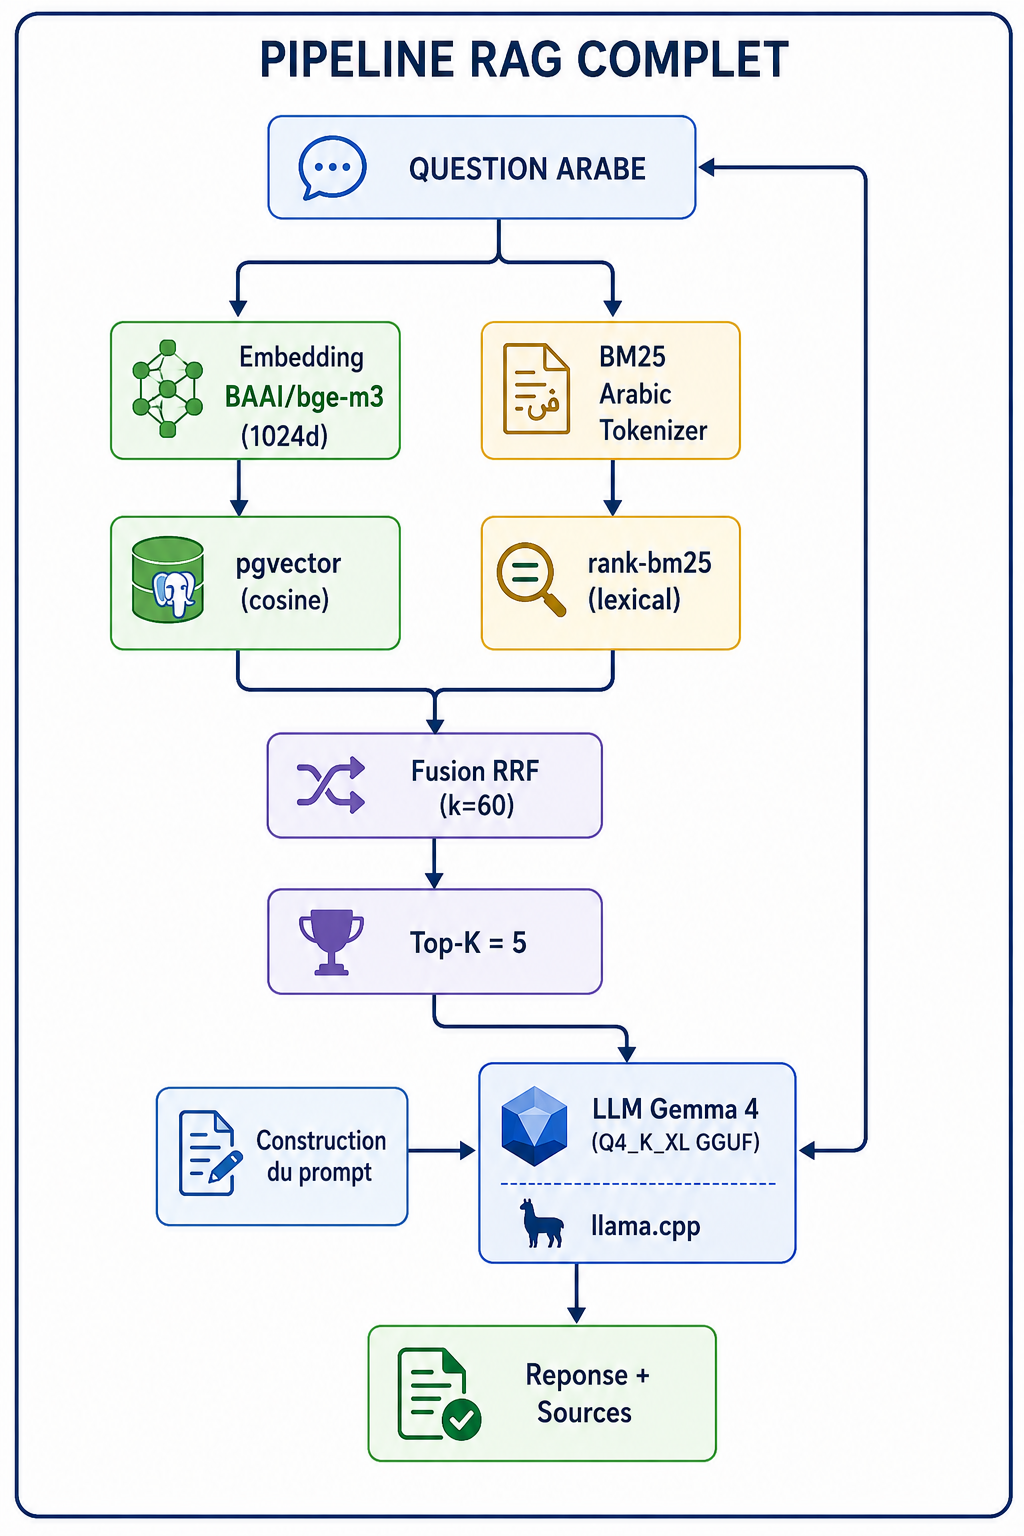
\includegraphics[width=0.6\textwidth]{images/illustrations/rag_pipeline_bge_m3.png}
    \caption{Complete hybrid Retrieval-Augmented Generation (RAG) pipeline for Arabic question answering.}
    \label{fig:hybrid-rag-pipeline}
\end{figure}


Cette approche garantit que chaque reponse est \textbf{tracable et verifiable} : l'utilisateur peut consulter les articles originaux ayant servi a la generation, et l'enrichissement contextuel (synthese, verdicts, references croisees) est explicitement distingue des hallucinations car ancre dans les sources.

\section{Technologies Utilisees}

Le systeme repose sur une stack technologique moderne et open-source, optimisee pour le deploiement sur materiel modeste :

\begin{itemize}
    \item \textbf{Extraction de texte} : PyMuPDF, pdfplumber, EasyOCR (reconnaissance arabe)
    \item \textbf{Correction OCR} : Modele de vision (VLM) Gemma 4 pour correction des erreurs de reconnaissance
    \item \textbf{Traitement du langage arabe} : Normalisation Unicode (NFKC), unification des alefs, suppression des tatweel, segmentation en articles, tokenizer arabe avec 60+ stop words juridiques
    \item \textbf{Modeles d'embedding} : intfloat/multilingual-E5-large (1024 dimensions, 560M parametres), BGE-M3 en alternative
    \item \textbf{Base de donnees vectorielle} : PostgreSQL 16 + pgvector 0.7.4 (indexation HNSW, m=16, ef\_construction=200)
    \item \textbf{Recherche hybride} : Similarite cosinus vectorielle + BM25 avec tokenizer arabe, fusion par Reciprocal Rank Fusion (RRF, k=60)
    \item \textbf{Modele de langage} : Gemma 4 2B parametres, quantifie Q4\_K\_XL (GGUF, $\sim$1.1 Go), inference via llama.cpp
    \item \textbf{Service d'embedding distant} : Google Colab (GPU T4) + Cloudflare Tunnel pour l'embedding GPU, fallback CPU local
    \item \textbf{API Backend} : FastAPI (Python), endpoints REST (/search, /ask, /laws, /upload)
    \item \textbf{Frontend} : SvelteKit 5 + Tailwind CSS 4 + TypeScript
    \item \textbf{Infrastructure} : Docker Compose (PostgreSQL + pgAdmin), Cloudflare Tunnel, llama.cpp
\end{itemize}

\section{Domaines Juridiques Couverts}

Le systeme couvre sept domaines du droit marocain, avec un corpus d'environ 2 357 articles structures :

\begin{multicols}{2}
\begin{itemize}
    \item Droit Penal --- \textit{\textarabic{القانون الجنائي}} (822 articles)
    \item Code de la Route --- \textit{\textarabic{مدونة السير}} (228 articles)
    \item Droit Civil --- \textit{\textarabic{قانون الالتزامات والعقود}} (705 articles)
    \item Droit Commercial --- \textit{\textarabic{مدونة التجارة}} (359 articles)
    \item Procedures Judiciaires --- \textit{\textarabic{التنظيم القضائي}} (32 articles)
    \item Droit Fiscal --- \textit{\textarabic{المدونة العامة للضرائب}} (211 articles)
    \item Contraventions et Sanctions --- \textit{\textarabic{قانون المخالفات والعقوبات}}
\end{itemize}
\end{multicols}

\chapter{Etat de l'Art}

\section{Introduction}

Ce chapitre presente une revue de la litterature couvrant les domaines fondamentaux sur lesquels repose le projet Moroccan Legal RAG. Nous abordons successivement le traitement automatique du langage arabe (Arabic NLP), les systemes de recherche d'information juridique (Legal IR), l'architecture Retrieval-Augmented Generation (RAG), les techniques de quantification de LLMs pour le deploiement leger, et les defis specifiques au traitement des documents juridiques marocains.

\section{Traitement Automatique de la Langue Arabe (Arabic NLP)}

\subsection{Particularites Linguistiques de l'Arabe}

La langue arabe presente des defis uniques pour le traitement automatique :

\begin{itemize}
    \item \textbf{Morphologie complexe} : L'arabe est une langue a morphologie riche. Un meme mot peut prendre de nombreuses formes selon le genre, le nombre, la personne, le temps, et le mode. Par exemple, le verbe \textit{kataba} (ecrire) peut generer des dizaines de formes derivees.
    
    \item \textbf{Systeme de racines} : La plupart des mots arabes derivent de racines trilitteres (trois consonnes). Les mots partageant la meme racine sont semantiquement lies, ce qui constitue a la fois une opportunite (regroupement semantique) et un defi (ambiguite).
    
    \item \textbf{Diacritiques} : Les signes diacritiques (\textit{tashkil}) indiquent les voyelles courtes et modifient le sens des mots. Leur presence est irreguliere dans les textes juridiques, ou ils apparaissent principalement pour lever des ambiguites.
    
    \item \textbf{Diglossie} : Le monde arabe est caracterise par une situation de diglossie ou coexistent l'arabe standard moderne (MSA, utilise a l'ecrit et dans les contextes formels) et les dialectes regionaux comme le darija marocain. Dans le domaine juridique, l'arabe standard predomine, mais les citoyens utilisent le darija pour formuler leurs questions.
\end{itemize}

\subsection{Normalisation et Pretraitement}

Les travaux de \textsc{Darwish} (2014) et \textsc{Al-Khalifa} (2019) ont etabli les fondements de la normalisation du texte arabe pour la recherche d'information. Les etapes essentielles appliquees dans le cadre de ce projet comprennent :

\begin{enumerate}
    \item \textbf{Unification des variantes de l'alef} : Les caracteres \textit{alef} (\begin{otherlanguage}{arabic}ا\end{otherlanguage}), \textit{alef avec hamza} (\begin{otherlanguage}{arabic}أ\end{otherlanguage}, \begin{otherlanguage}{arabic}إ\end{otherlanguage}), et \textit{alef madda} (\begin{otherlanguage}{arabic}آ\end{otherlanguage}) sont unifies en \begin{otherlanguage}{arabic}ا\end{otherlanguage}.
    \item \textbf{Suppression du tatweel} : Le caractere d'allongement \textit{kashida} (\begin{otherlanguage}{arabic}ـ\end{otherlanguage}) est supprime pour eviter la fragmentation des mots.
    \item \textbf{Suppression des diacritiques} : Les voyelles courtes sont retirees, sauf dans les cas ou leur presence modifie le sens juridique.
    \item \textbf{Normalisation Unicode} : Application des formes de normalisation NFKC pour uniformiser les codages equivalents.
    \item \textbf{Tokenisation arabe specialisee} : Un tokenizer dedie avec 60+ stop words juridiques a ete developpe pour isoler les termes discriminants (noms de lois, concepts juridiques, numeros d'articles).
\end{enumerate}

\subsection{Modeles de Langue et d'Embedding pour l'Arabe}

L'avenement des modeles de langue pre-entraines a considerablement fait progresser le NLP arabe :

\begin{itemize}
    \item \textbf{AraBERT} (\textsc{Antoun et al.}, 2020) : Base sur l'architecture BERT, pre-entraine sur un corpus de textes arabes modernes. Performances etat-de-l'art sur les taches de classification et d'extraction d'information en arabe standard.
    
    \item \textbf{CAMeL-Tools} (\textsc{Obeid et al.}, 2020) : Suite d'outils open-source pour le NLP arabe developpee par le CAMeL Lab. Inclut la tokenisation, la lemmatisation, et l'analyse morphologique -- utilisee comme reference dans ce projet.
    
    \item \textbf{Multilingual-E5-large} (\textsc{Wang et al.}, 2024) : Modele d'embedding multilingue de 560 millions de parametres produisant des vecteurs de dimension 1024. Selectionne comme modele principal de ce projet apres un benchmark systematique de 5 modeles sur 65 variantes de requetes juridiques. Il a obtenu les meilleurs scores (P@5 = 0.72, MRR = 0.81) sur l'arabe juridique marocain.
    
    \item \textbf{BGE-M3} (\textsc{Chen et al.}, 2024) : Modele d'embedding multilingue de 568 millions de parametres (1024 dimensions), utilise comme alternative dans notre pipeline. Performances legerement inferieures a E5-large sur le corpus juridique marocain (P@5 = 0.69).
    
    \item \textbf{LaBSE} (\textsc{Feng et al.}, 2022) : Modele d'embedding de 768 dimensions, excellent pour le francais juridique -- utilise comme modele de fallback CPU.
\end{itemize}

\section{Recherche d'Information Juridique (Legal IR)}

\subsection{Systemes Traditionnels}

La recherche d'information juridique a historiquement repose sur des approches booleennes et des index inverses. Les systemes commerciaux comme \textit{Westlaw}, \textit{LexisNexis}, et \textit{Doctrine.fr} utilisent des moteurs de recherche bases sur des mots-cles avec des filtres juridiques.

Au Maroc, les initiatives de numerisation du droit comprennent :

\begin{itemize}
    \item \textbf{ADALA} : Base de donnees juridique marocaine en ligne proposant un acces aux textes de loi, a la jurisprudence, et aux circulaires.
    \item \textbf{SGG (Secretariat General du Gouvernement)} : Portail officiel de publication des textes de loi au Bulletin Officiel.
    \item \textbf{Ministere de la Justice} : Portail de la legislation marocaine avec acces aux codes et lois.
\end{itemize}

Ces systemes reposent principalement sur la recherche par mots-cles et ne proposent ni recherche semantique, ni generation automatisee de reponses, ni ancrage dans les sources.

\subsection{Approches Neuronales}

Les travaux recents en Legal IR exploitent les modeles de langue neuronaux :

\begin{itemize}
    \item \textbf{Legal-BERT} (\textsc{Chalkidis et al.}, 2020) : BERT specialise pour le domaine juridique, pre-entraine sur des corpus legaux. Ameliorations significatives sur la classification de documents juridiques.
    
    \item \textbf{Caselaw Access Project} : Projet de numerisation et d'indexation de la jurisprudence americaine utilisant des techniques de NLP pour l'extraction de citations et la recherche semantique.
    
    \item \textbf{COLIEE} (Competition on Legal Information Extraction/Entailment) : Competition internationale annuelle evaluant les systemes de recherche d'information juridique et de raisonnement legal automatise.
\end{itemize}

\subsection{Limites de la Recherche Lexicale Pure}

Notre benchmark interne (32 questions reparties sur 7 domaines juridiques marocains) a revele que la recherche plein-texte PostgreSQL avec le dictionnaire arabe (\texttt{to\_tsvector(`arabic', ...)}) echoue systematiquement pour les requetes juridiques en arabe (0 resultat sur 32 questions). Ce constat a motive le developpement d'une recherche lexicale alternative basee sur \texttt{rank-bm25} avec un tokenizer arabe specialise integrant :

\begin{itemize}
    \item Extraction de mots par expression reguliere Unicode (plage arabe)
    \item Suppression de 60+ mots vides juridiques
    \item Normalisation prealable via l'\texttt{ArabicNormalizer} du projet
    \item Filtrage des tokens courts ($< 2$ caracteres)
\end{itemize}

\subsection{Recherche Hybride pour le Droit}

La specificite du langage juridique --- melant terminologie precise et concepts abstraits --- rend les approches hybrides particulierement pertinentes. \textsc{Shao et al.} (2023) ont demontre que la combinaison de recherche semantique (dense) et de recherche lexicale (BM25) via Reciprocal Rank Fusion (RRF) offrait les meilleurs resultats pour les requetes juridiques. Notre systeme implemente cette approche avec :

\begin{itemize}
    \item \textbf{Canal dense} : Similarite cosinus via pgvector (indexation HNSW, m=16)
    \item \textbf{Canal lexical} : BM25 avec le tokenizer arabe specialise
    \item \textbf{Fusion RRF} : Reciprocal Rank Fusion avec k=60, sans parametre a regler
\end{itemize}

\section{Architecture Retrieval-Augmented Generation (RAG)}

\subsection{Principe Fondamental}

L'architecture RAG, introduite par \textsc{Lewis et al.} (2020), combine un modele de recherche d'information (retriever) et un modele de generation de texte (generator). Le principe implemente dans ce projet est le suivant :

\begin{enumerate}
    \item \textbf{Ingestion} : Les documents juridiques (PDF) sont extraits par OCR, corriges par VLM, nettoyes, normalises, structures en articles, et transformes en vecteurs de 1024 dimensions (embedding E5-large) stockes dans PostgreSQL + pgvector.
    \item \textbf{Recherche hybride} : La requete en arabe est traitee simultanement par le canal dense (cosine similarity) et le canal lexical (BM25 avec tokenizer arabe), puis fusionnee par RRF.
    \item \textbf{Augmentation contextuelle} : Les K articles les plus pertinents sont inseres dans un prompt structure avec instruction de fidelite au contexte.
    \item \textbf{Generation enrichie} : Le LLM genere une reponse juridique complete en arabe (resume, analyse, verdict, sources) en s'appuyant exclusivement sur les articles fournis. L'enrichissement contextuel (synthese multi-sources, references croisees, conclusions juridiques) est un comportement souhaite et ancre, distinct de l'hallucination.
\end{enumerate}

\subsection{Avantages pour le Domaine Juridique}

L'architecture RAG presente des avantages decisifs pour les applications juridiques :

\begin{itemize}
    \item \textbf{Ancrage factuel} : Les reponses sont fondees sur des sources verifiables. Les enrichissements contextuels (verdicts, synthese) derivent des articles retrouves.
    \item \textbf{Tra\c{c}abilite} : Chaque reponse cite les numeros d'articles et les lois sources.
    \item \textbf{Mise a jour} : La base de connaissances peut etre mise a jour par simple re-indexation, sans re-entrainement du LLM.
    \item \textbf{Specialisation juridictionnelle} : Le systeme se limite aux textes de loi marocains, evitant les confusions avec d'autres droits nationaux.
\end{itemize}

\subsection{Travaux Connexes}

Plusieurs projets recents appliquent le paradigme RAG au domaine juridique :

\begin{itemize}
    \item \textbf{SAIL-Legal} (\textsc{Huang et al.}, 2024) : Systeme RAG pour le droit chinois utilisant une base de donnees vectorielle et un modele de langage specialise.
    
    \item \textbf{LexGPT} (\textsc{Zhou et al.}, 2023) : Assistant juridique base sur GPT-4 avec augmentation par recherche dans des bases de donnees juridiques.
    
    \item \textbf{Indian Legal RAG} (\textsc{Sharma et al.}, 2024) : Systeme RAG pour le droit indien integrant la recherche semantique multilingue (anglais et hindi).
\end{itemize}

Aucun de ces systemes ne traite specifiquement le droit marocain en langue arabe avec une architecture legerement deployable (LLM quantifie, Docker Compose), ce qui constitue la contribution originale de ce projet.

\section{Quantification de LLMs pour le Deploiement Leger}

\subsection{Principe de la Quantification}

Les modeles de langage modernes contiennent des milliards de parametres en virgule flottante (FP16, FP32), rendant leur deploiement couteux en memoire et en calcul. La quantification reduit la precision des poids du modele pour diminuer l'empreinte memoire et accelerer l'inference :

\begin{itemize}
    \item \textbf{FP16 (origine)} : 2 octets par parametre. Un modele de 2B parametres occupe $\sim$4 Go en memoire.
    \item \textbf{INT8 (Q8\_0)} : 1 octet par parametre. Memoire divisee par 2, perte de qualite negligeable ($< 0.5\%$).
    \item \textbf{INT4 (Q4\_K\_XL)} : 0.5 octet par parametre. Memoire divisee par 4, perte de qualite maitrisee ($< 2\%$).
\end{itemize}

\subsection{Format GGUF et llama.cpp}

Le format \textbf{GGUF} (GPT-Generated Unified Format), introduit par la communaute llama.cpp, est devenu le standard de facto pour la distribution de modeles quantifies :

\begin{itemize}
    \item \textbf{Portabilite} : Un seul fichier contenant les poids, la configuration, et le tokenizer.
    \item \textbf{Inference CPU+GPU hybride} : llama.cpp repartit automatiquement les couches entre CPU et GPU selon la memoire disponible.
    \item \textbf{Formats de quantification} : Q2\_K a Q8\_0, avec des variantes optimisees (K\_S, K\_M, K\_L, K\_XL) pour differents compromis vitesse/qualite.
\end{itemize}

\subsection{Application au Projet}

Dans le cadre de ce projet, le modele \textbf{Gemma 4 2B} (Google, 2025) a ete selectionne et quantifie en Q4\_K\_XL :

\begin{itemize}
    \item \textbf{Taille originale (FP16)} : $\sim$4 Go
    \item \textbf{Taille quantifiee (Q4\_K\_XL)} : $\sim$1.1 Go (reduction de 73\%)
    \item \textbf{Inference} : llama.cpp avec GPU layers = -1 (tous sur GPU T4 Colab, $\sim$2-5s par generation)
    \item \textbf{Contexte maximal} : 16 384 tokens
    \item \textbf{Temperature} : 0.3 (favorisant la fidelite au contexte sur la creativite)
\end{itemize}

Cette configuration permet un deploiement sur du materiel modeste (GPU T4 gratuit via Google Colab, ou CPU local pour les tests) tout en maintenant une qualite de generation acceptable pour des reponses juridiques structurees et tracables.

\section{Traitement des Documents PDF Juridiques Marocains}

\subsection{Defis Specifiques}

L'extraction de texte a partir de documents PDF juridiques marocains presente des defis uniques qui ont guide les choix techniques du projet :

\begin{itemize}
    \item \textbf{Documents numerises} : La majorite des textes de loi marocains existent uniquement sous forme de scans (Bulletins Officiels), necessitant une etape d'OCR. Le projet utilise EasyOCR avec acceleration GPU pour la reconnaissance du texte arabe.
    
    \item \textbf{Mise en page complexe} : Les documents officiels utilisent des mises en page multi-colonnes, avec en-tetes, pieds de page, et notes marginales -- necessitant un nettoyage structurel (LegalTextCleaner) avant la normalisation.
    
    \item \textbf{Mixite linguistique} : Les documents contiennent de l'arabe et du francais sur la meme page, exigeant une segmentation par detection de script Unicode.
    
    \item \textbf{Qualite variable} : Les scans historiques peuvent etre degrades. Pour y remedier, le projet utilise un modele de vision (VLM) --- Gemma 4 en mode vision --- pour corriger les erreurs de reconnaissance post-OCR.
\end{itemize}

\subsection{Correction Post-OCR par VLM}

Les travaux de \textsc{Benajiba et al.} (2023) sur la correction post-OCR pour l'arabe ont identifie les erreurs frequentes :

\begin{itemize}
    \item Confusion entre caracteres visuellement similaires (\begin{otherlanguage}{arabic}ت\end{otherlanguage} / \begin{otherlanguage}{arabic}ث\end{otherlanguage} / \begin{otherlanguage}{arabic}ب\end{otherlanguage})
    \item Segmentation incorrecte des mots lies
    \item Omission ou insertion de points diacritiques
    \item Inversion de l'ordre des caracteres dans les textes bidirectionnels
\end{itemize}

Notre approche de correction utilise un prompt VLM specialise : \textit{<Corrige UNIQUEMENT les erreurs de reconnaissance optique. NE TRADUIS PAS. NE RESUMES PAS.>} Le traitement est effectue article par article avec un systeme de checkpoint/reprise pour les longs documents.

\section{Segmentation et Chunking des Textes Juridiques}

La segmentation des textes de loi en unites exploitables est critique pour la qualite de la recherche. Les approches evaluees sont :

\begin{itemize}
    \item \textbf{Segmentation par article} : Decoupage aux frontieres des articles (\textit{المادة X}). Cette approche, retenue pour le projet, preserve l'integrite semantique de chaque disposition legale et facilite la citation dans les reponses generees.
    \item \textbf{Segmentation par clause} : Decoupage au niveau des alineas, non retenu car trop fragmentaire pour le contexte juridique.
    \item \textbf{Segmentation par fenetre} : Approche de secours pour les documents sans structure explicite.
\end{itemize}

\section{Synthese et Positionnement du Projet}

L'etat de l'art revele plusieurs constats determinants pour le positionnement du projet :

\begin{enumerate}
    \item \textbf{Absence de systeme RAG pour le droit marocain en arabe} : Aucun travail academique ou commercial n'a applique l'architecture RAG au corpus juridique marocain avec une stack exclusivement arabophone.

    \item \textbf{Insuffisance des outils standards pour l'arabe juridique} : Les dictionnaires PostgreSQL arabic et les tokenizers naifs (split sur espaces) echouent systematiquement sur le corpus juridique, motivant le developpement d'outils specialises (tokenizer arabe avec 60+ stop words juridiques, normaliseur dedie).

    \item \textbf{Maturite des embeddings multilingues} : Les modeles E5-large et BGE-M3 atteignent des performances suffisantes pour la recherche semantique juridique en arabe (P@5 $\sim$72\%, MRR $\sim$81\% sur notre benchmark).

    \item \textbf{Viabilite de la quantification pour le deploiement} : La quantification GGUF Q4\_K\_XL permet de deployer un LLM de 2B parametres sur GPU modeste ($\sim$1.1 Go) avec une perte de qualite acceptable ($< 2\%$).

    \item \textbf{Pertinence de la recherche hybride} : La combinaison de recherche semantique (dense) et lexicale (BM25 avec tokenizer arabe) via RRF est particulierement adaptee aux requetes juridiques, combinant comprehension semantique et precision terminologique.

    \item \textbf{Enrichissement contextuel vs hallucination} : Dans le domaine juridique, la synthese multi-sources, les references croisees d'articles, et la formulation de verdicts sont des comportements souhaites du LLM, a condition qu'ils soient ancres dans les documents retrouves. La distinction entre enrichissement contextuel legitime et hallucination constitue un axe de recherche identifie mais non resolu par les metriques standard (token-overlap).
\end{enumerate}

Le projet \textbf{Moroccan Legal RAG} se positionne comme la premiere application de l'architecture RAG au droit marocain en langue arabe, integrant :

\begin{itemize}
    \item Un pipeline complet d'ingestion : PDF scanne $\to$ EasyOCR $\to$ correction VLM $\to$ nettoyage $\to$ normalisation arabe $\to$ structuration en articles
    \item Une recherche hybride (dense + BM25 arabe + RRF) avec tokenisation adaptee
    \item Un LLM leger quantifie (Gemma 4 2B, Q4\_K\_XL GGUF, llama.cpp) deployable sur materiel modeste
    \item Une evaluation systematique via un benchmark de 32 questions sur 7 domaines juridiques, avec 5 metriques (Precision, Recall, MRR, Relevance, Faithfulness)
    \item Une interface web (SvelteKit) et une API REST (FastAPI) operationnelles
    \item Une infrastructure conteneurisee (Docker Compose) avec service d'embedding GPU distant (Colab + Cloudflare Tunnel)
\end{itemize}
\chapter{Conception du Systeme}

\section{Architecture Globale}

Le systeme Moroccan Legal RAG est concu selon une architecture modulaire en couches, ou chaque composant est independant et communicant via des interfaces bien definies. L'architecture suit le paradigme RAG (Retrieval-Augmented Generation) avec une strategie de recherche hybride associant similarite semantique dense et recherche lexicale BM25.

\subsection{Vue d'Ensemble}

L'architecture globale s'articule autour de cinq couches principales :

\begin{enumerate}
    \item \textbf{Couche Ingestion} : Extraction du texte depuis les documents sources (PDF), correction OCR, nettoyage, normalisation arabe, et structuration en articles.
    \item \textbf{Couche Stockage} : Base de donnees PostgreSQL 16 avec l'extension pgvector 0.7.4 pour le stockage des articles et de leurs vecteurs semantiques (embeddings).
    \item \textbf{Couche Recherche} : Moteur de recherche hybride combinant similarite cosinus (dense) et BM25 avec tokenizer arabe specialise, fusionnes par Reciprocal Rank Fusion (RRF).
    \item \textbf{Couche Generation} : Modele de langage Gemma 4 (2B parametres, quantifie Q4\_K\_XL GGUF) pour la generation de reponses juridiques ancrees dans les articles retrouves.
    \item \textbf{Couche Presentation} : API REST (FastAPI), interface web (SvelteKit 5 + Tailwind CSS 4), et interface terminal (Textual).
\end{enumerate}

\begin{figure}[H]
    \centering
    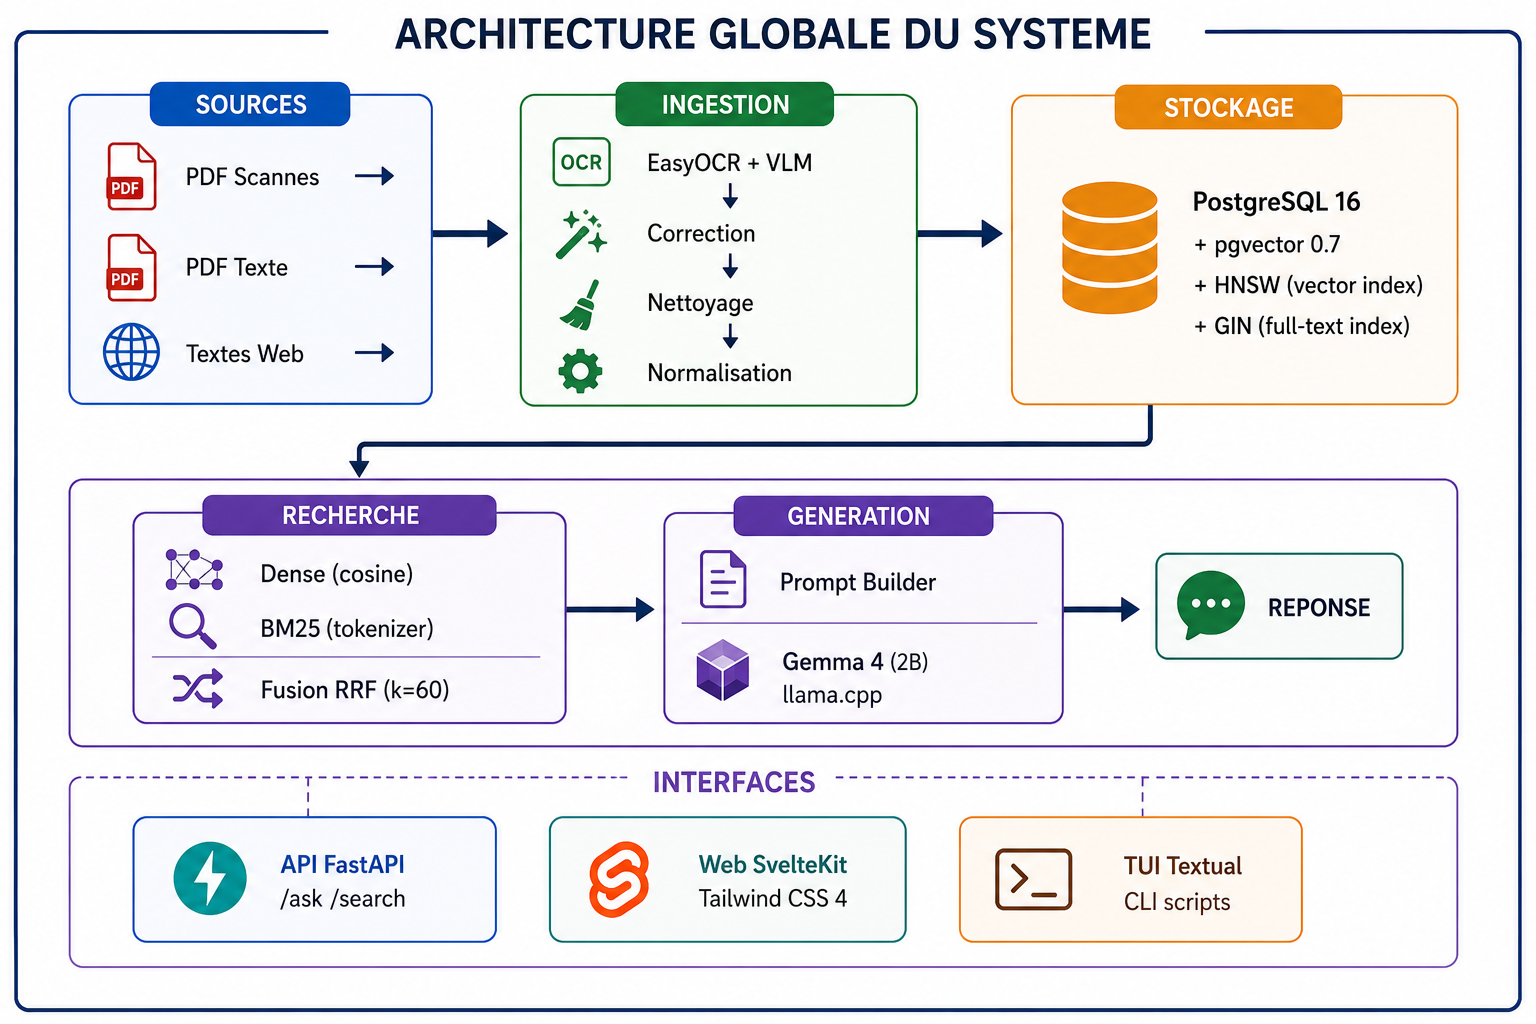
\includegraphics[width=\textwidth]{images/illustrations/architecture_globale_systeme.png}
    \caption{Overall architecture of the legal RAG system, showing the document ingestion workflow, storage layer, hybrid retrieval engine, response generation pipeline, and user-facing interfaces.}
    \label{fig:global-architecture}
\end{figure}

La Figure~\ref{fig:flux-donnees} (Section~\ref{sec:flux-donnees}) detaille le cheminement complet d'une requete a travers ces couches.

\subsection{Stack Technique Detaillee}

Le tableau~\ref{tab:stack-technique} resume les technologies retenues pour chaque couche du systeme :

\begin{table}[h]
\centering
\renewcommand{\arraystretch}{1.3}
\begin{tabular}{|l|l|l|}
\hline
\rowcolor{LightBlue}
\textbf{\color{PrimaryBlue}Couche} & \textbf{\color{PrimaryBlue}Technologie} & \textbf{\color{PrimaryBlue}Role} \\
\hline
Extraction PDF & PyMuPDF, pdfplumber & Rendu et extraction de texte \\
OCR & EasyOCR (GPU) & Reconnaissance de l'arabe imprime \\
Correction OCR & Gemma 4 (mode VLM) & Correction des erreurs de reconnaissance \\
Nettoyage & LegalTextCleaner & Suppression bruit structurel \\
Normalisation & ArabicNormalizer & Unification alef, tatweel, diacritiques \\
Structuration & LegalStructureParser & Decoupage en articles avec metadonnees \\
\hline
Embedding & E5-large (1024d, 560M) & Vectorisation semantique des articles \\
Base de donnees & PostgreSQL 16 + pgvector 0.7.4 & Stockage articles + vecteurs \\
Index vectoriel & HNSW (m=16) & Recherche par similarite rapide \\
Index lexical & BM25Okapi + tokenizer arabe & Recherche par mots-cles \\
\hline
Fusion & RRF (k=60) & Combinaison dense + lexical \\
Generation & Gemma 4 2B (Q4\_K\_XL GGUF) & Reponses juridiques en arabe \\
Inference LLM & llama.cpp & CPU + GPU hybride \\
Service distant & Cloudflare Tunnel & Exposition Colab GPU \\
\hline
API & FastAPI (Python) & Endpoints REST \\
Frontend Web & SvelteKit 5 + Tailwind CSS 4 & Interface utilisateur \\
TUI & Textual (Python) & Gestion du corpus en terminal \\
Infrastructure & Docker Compose & Conteneurisation \\
\hline
\end{tabular}
\caption{Stack technique complete du systeme Moroccan Legal RAG}
\label{tab:stack-technique}
\end{table}

\section{Flux de Donnees Principal}
\label{sec:flux-donnees}

Le flux de donnees decrit le cheminement d'une question utilisateur depuis sa soumission jusqu'a la generation de la reponse juridique (Figure~\ref{fig:flux-donnees}) :

\begin{figure}[h]
    \centering
    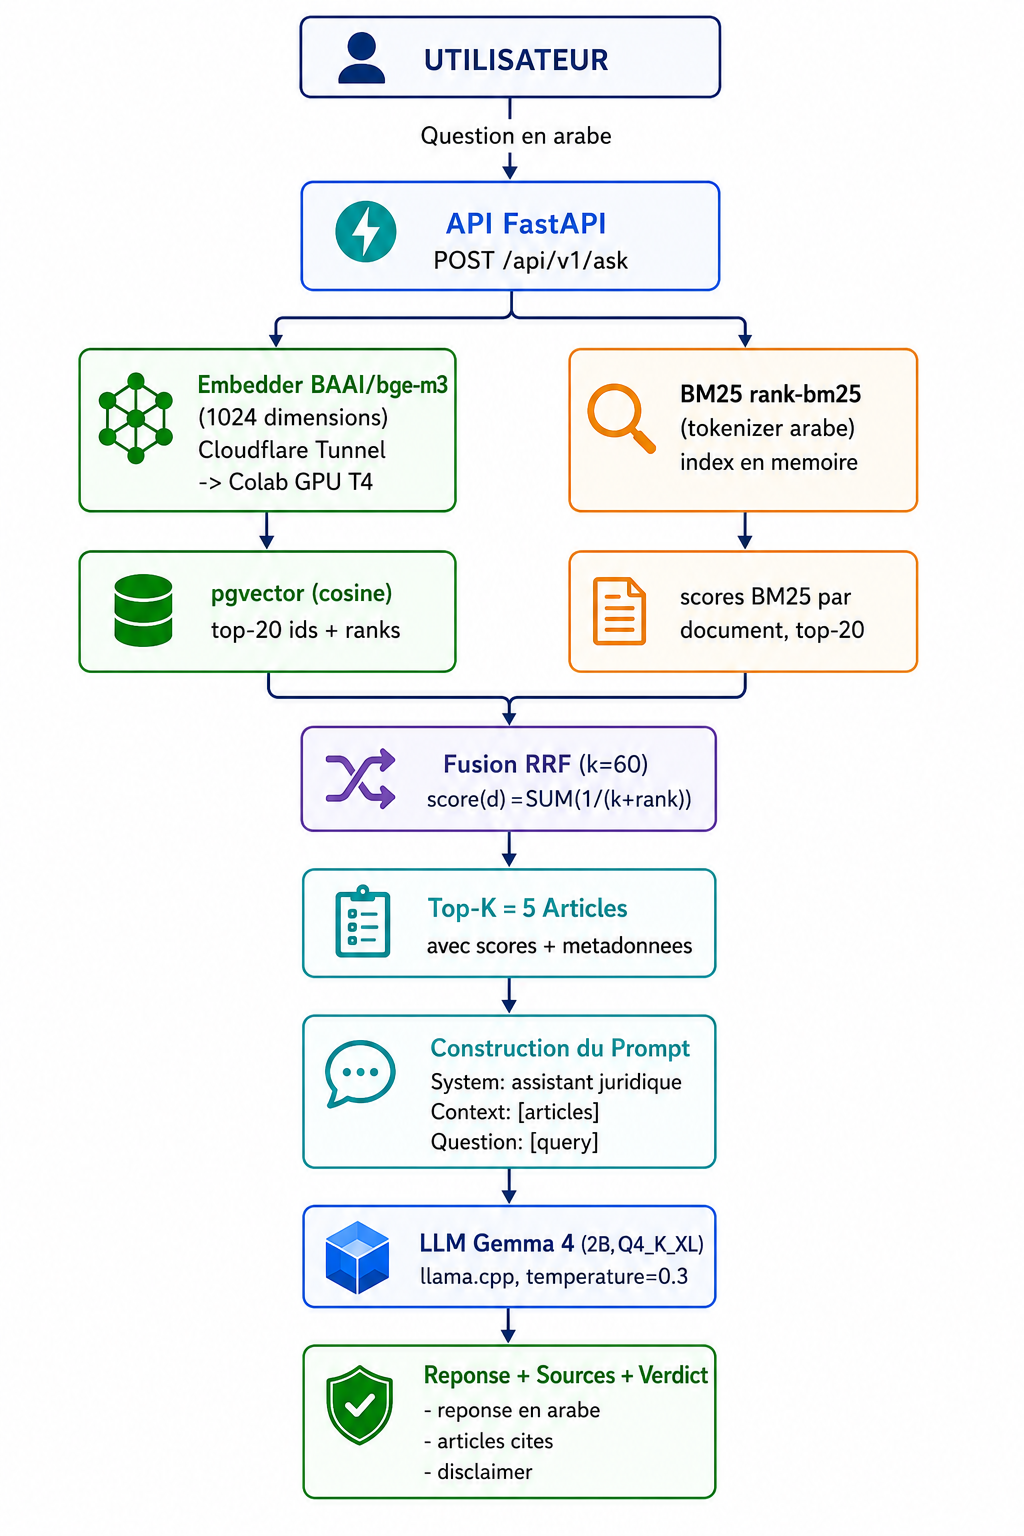
\includegraphics[width=0.85\textwidth]{images/illustrations/rag_dataflow_bge_m3.png}
    \caption{End-to-end data flow of the legal RAG system, combining dense retrieval using BAAI/bge-m3 embeddings and sparse BM25 retrieval through Reciprocal Rank Fusion (RRF) before answer generation with Gemma 4.}
    \label{fig:flux-donnees}
\end{figure}

\section{Phase 1 -- Collecte et Constitution du Corpus}

\subsection{Sources de Donnees}

Le corpus juridique marocain a ete constitue a partir de trois types de sources :

\begin{itemize}
    \item \textbf{Bulletins Officiels (PDF numerises)} : Publication officielle des textes de loi au Maroc. Ces documents sont des scans de qualite variable necessitant une etape d'OCR.
    \item \textbf{PDF natifs} : Certains textes recents sont disponibles en format PDF avec texte selectionnable, permettant une extraction directe.
    \item \textbf{Portails gouvernementaux} : Textes publies sur les sites du SGG, du Ministere de la Justice, et d'ADALA.
\end{itemize}

\subsection{Pipeline d'Extraction}

Le pipeline d'extraction (Figure~\ref{fig:pipeline-extraction}) automatise le passage du PDF brut a l'article structure :

\begin{figure}[H]
    \centering
    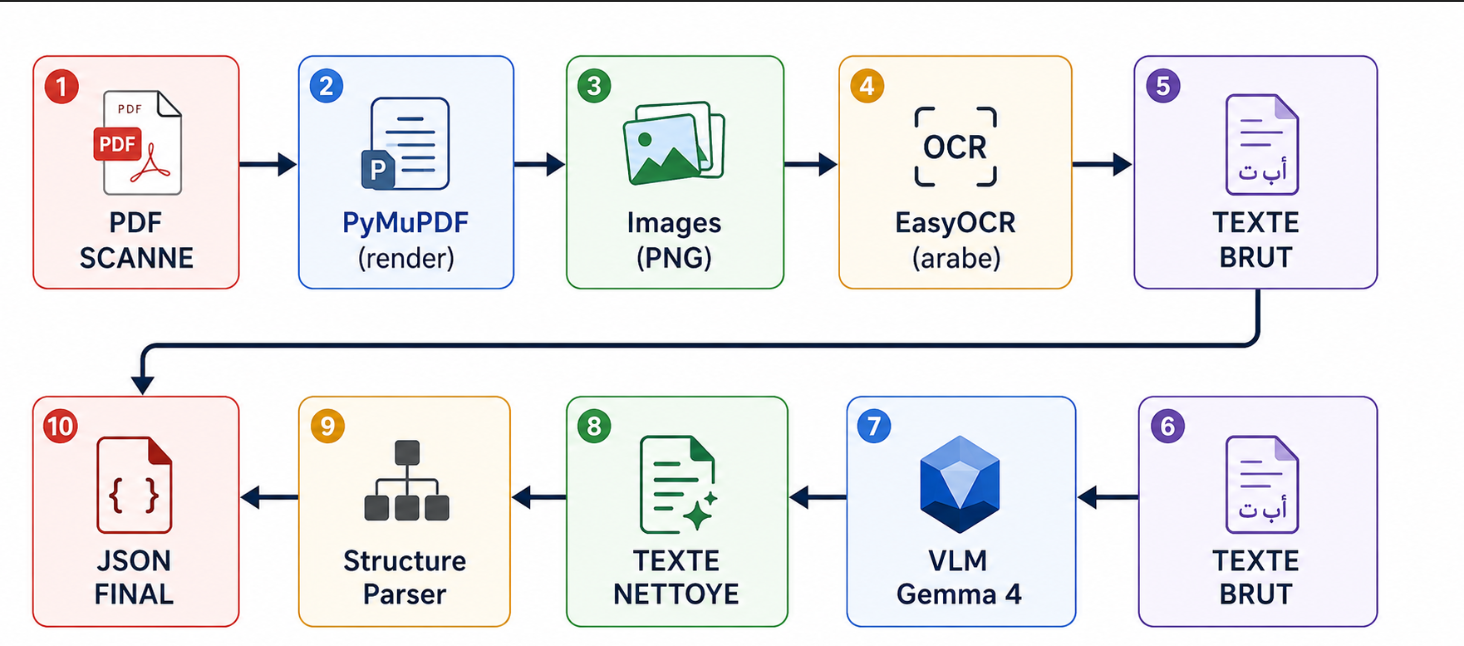
\includegraphics[width=\textwidth]{images/illustrations/pipeline_extraction.png}
    \caption{Document extraction pipeline transforming scanned PDF files into structured JSON articles through OCR, text cleaning, vision-language processing, and schema parsing.}
    \label{fig:pipeline-extraction}
\end{figure}

\subsection{Etapes du Pipeline}

\begin{enumerate}
    \item \textbf{Rendu PDF} : PyMuPDF (fitz) convertit chaque page du PDF en image PNG.
    \item \textbf{OCR} : EasyOCR effectue la reconnaissance du texte arabe sur les images.
    \item \textbf{Correction VLM} : Gemma 4 en mode vision corrige les erreurs de reconnaissance avec un prompt specialise (\textit{«~Corrige UNIQUEMENT les erreurs d'OCR. NE TRADUIS PAS. NE RESUMES PAS.~»}).
    \item \textbf{Nettoyage structurel} : LegalTextCleaner supprime les en-tetes, pieds de page, numeros de page, et les artefacts de numerisation.
    \item \textbf{Normalisation arabe} : ArabicNormalizer unifie les variantes de caracteres (alefs, tatweel, diacritiques) et applique la normalisation Unicode NFKC.
    \item \textbf{Structuration} : LegalStructureParser detecte les motifs \textit{«~\textarabic{المادة} $X$~»} pour delimiter les articles et extraire les metadonnees (chapitre, section, loi).
    \item \textbf{Export JSON} : Chaque article est exporte au format JSON structure avec metadonnees.
\end{enumerate}

\subsection{Structure d'un Article (JSON)}

Chaque article du corpus est represente par le schema JSON du Listing~\ref{lst:article-json} :

\begin{jsonblock}{Document JSON --- Exemple d'article indexé}
\{\\
\quad "article\_number": "513",\\
\quad "law\_name": "code penal maroc ar",\\
\quad "domain": "criminal",\\
\quad "chapter\_title": "\textarabic{حماية الاحداث}",\\
\quad "section\_title": "\textarabic{التدابير الوقائية}",\\
\quad "text": "\textarabic{يعتبر الحدث البالغ من العمر اقل من 16 سنة...}",\\
\quad "source\_file": "code-penal-maroc-ar.pdf",\\
\quad "page\_number": 145\\
\}
\end{jsonblock}
\label{lst:article-json}
\subsection{Corpus Constitue}

Le corpus final est organise par domaine juridique et totalise environ 2\,357 articles (Tableau~\ref{tab:corpus-domaines}) :

\begin{table}[h]
\centering
\renewcommand{\arraystretch}{1.3}
\begin{tabular}{|l|r|r|}
\hline
\rowcolor{LightBlue}
\textbf{\color{PrimaryBlue}Domaine} & \textbf{\color{PrimaryBlue}Articles} & \textbf{\color{PrimaryBlue}Lois principales} \\
\hline
Droit Penal & 822 & Code Penal, Code des Sanctions \\
Circulation & 228 & Code de la Route \\
Droit Civil & 705 & Code des Obligations, Procedure Civile, Impots \\
Droit Commercial & 359 & Registre du Commerce, Droit des Societes \\
Organisation Judiciaire & 32 & Loi 38.15, Carte Judiciaire \\
Droit Fiscal & 211 & Code General des Impots 2024 \\
\hline
\textbf{Total} & \textbf{2\,357} & \\
\hline
\end{tabular}
\caption{Repartition du corpus par domaine juridique}
\label{tab:corpus-domaines}
\end{table}

\section{Phase 2 -- Traitement et Validation des Donnees}

\subsection{Module de Nettoyage (LegalTextCleaner)}

Le module de nettoyage elimine le bruit structurel du texte extrait avant la normalisation linguistique. Il applique les regles suivantes, configurables via \texttt{config/cleaning.yaml} :

\begin{itemize}
    \item Suppression des en-tetes et pieds de page recurrents
    \item Normalisation des espaces et suppression des lignes vides
    \item Correction des retours a la ligne intempestifs en milieu de phrase
    \item Suppression des caracteres parasites de numerisation
    \item Detection et suppression des filigranes (\textit{watermarks})
    \item Deduplication des paragraphes repetes
\end{itemize}

\subsection{Module de Normalisation Arabe (ArabicNormalizer)}

Le normaliseur arabe standardise le texte au niveau des caracteres pour reduire la variabilite et ameliorer la qualite de l'embedding et de la recherche lexicale. Les regles appliquees incluent :

\begin{itemize}
    \item \textbf{Normalisation Unicode NFKC} : Uniformisation des codages equivalents
    \item \textbf{Unification des alefs} : \textarabic{أ}, \textarabic{إ}, \textarabic{آ} $\to$ \textarabic{ا}
    \item \textbf{Suppression du tatweel} : \textarabic{ـ} (kashida) supprime
    \item \textbf{Suppression des diacritiques} : Sauf \textit{shadda} (\textarabic{ّ}) preservee en option
    \item \textbf{Unification de la ponctuation} : Standardisation des separateurs
    \item \textbf{Unification des chiffres} : Chiffres arabo-indiens $\to$ chiffres ASCII
\end{itemize}

\subsection{Module de Structuration (LegalStructureParser)}

Le parser de structure identifie la hierarchie du document juridique :

\begin{itemize}
    \item \textbf{Niveau Article} : Motif \textit{«~\textarabic{المادة} $X$~»} -- delimite chaque article
    \item \textbf{Niveau Chapitre} : Motif \textit{«~\textarabic{الباب} $Y$~»} -- regroupe les articles
    \item \textbf{Niveau Section} : Motif \textit{«~\textarabic{القسم} $Z$~»} -- subdivision du chapitre
    \item \textbf{Niveau Livre} : Motif \textit{«~\textarabic{الكتاب} $W$~»} -- division majeure du code
\end{itemize}

Chaque article herite des metadonnees de son contexte hierarchique (chapitre, section, livre), facilitant la recherche contextuelle.

\subsection{Defis et Solutions}

Les defis rencontres lors du traitement des documents juridiques marocains et les solutions appliquees sont synthetises dans le Tableau~\ref{tab:defis-solutions} :

\begin{table}[h]
\centering
\renewcommand{\arraystretch}{1.3}
\begin{tabular}{|p{3.5cm}|p{3.5cm}|p{4.5cm}|}
\hline
\rowcolor{LightBlue}
\textbf{\color{PrimaryBlue}Probleme} & \textbf{\color{PrimaryBlue}Cause} & \textbf{\color{PrimaryBlue}Solution} \\
\hline
Bruit OCR & Scans de qualite degradee & Correction VLM + regles de nettoyage \\
Texte duplique & Repetitions dans les PDF sources & Detection par hash MD5 + similarite cosinus \\
Melange arabe/francais & Documents multilingues & Segmentation par detection de script Unicode \\
Metadonnees manquantes & Absence de structure explicite & Inference par heuristiques (motifs dans le texte) \\
Formatage irregulier & Heterogeneite des sources & Normalisation configurable via YAML \\
\hline
\end{tabular}
\caption{Defis rencontres et solutions appliquees lors du traitement des donnees}
\label{tab:defis-solutions}
\end{table}

\section{Modelisation de la Base de Donnees}

\subsection{Choix de PostgreSQL + pgvector}

Le choix de PostgreSQL 16 avec l'extension pgvector 0.7.4 repose sur plusieurs criteres decisifs :

\begin{itemize}
    \item \textbf{Unification} : Un seul systeme pour les donnees relationnelles (articles, metadonnees, conversations) et vectorielles (embeddings).
    \item \textbf{Transactions ACID} : Garantie de coherence entre l'insertion d'un article et son embedding.
    \item \textbf{Indexation HNSW} : Recherche vectorielle haute performance (m=16, ef\_construction=200).
    \item \textbf{Full-text search} : Bien que limite pour l'arabe, le tsvector PostgreSQL reste utile pour les metadonnees en francais.
    \item \textbf{Maturite et outillage} : 30+ ans d'existence, pgAdmin, pg\_dump, replication.
\end{itemize}

\subsection{Schema de la Base de Donnees}

Le schema de la base de donnees \texttt{legal\_rag} est presente dans la Figure~\ref{fig:schema-db} :

\begin{figure}[H]
\centering
\centering
    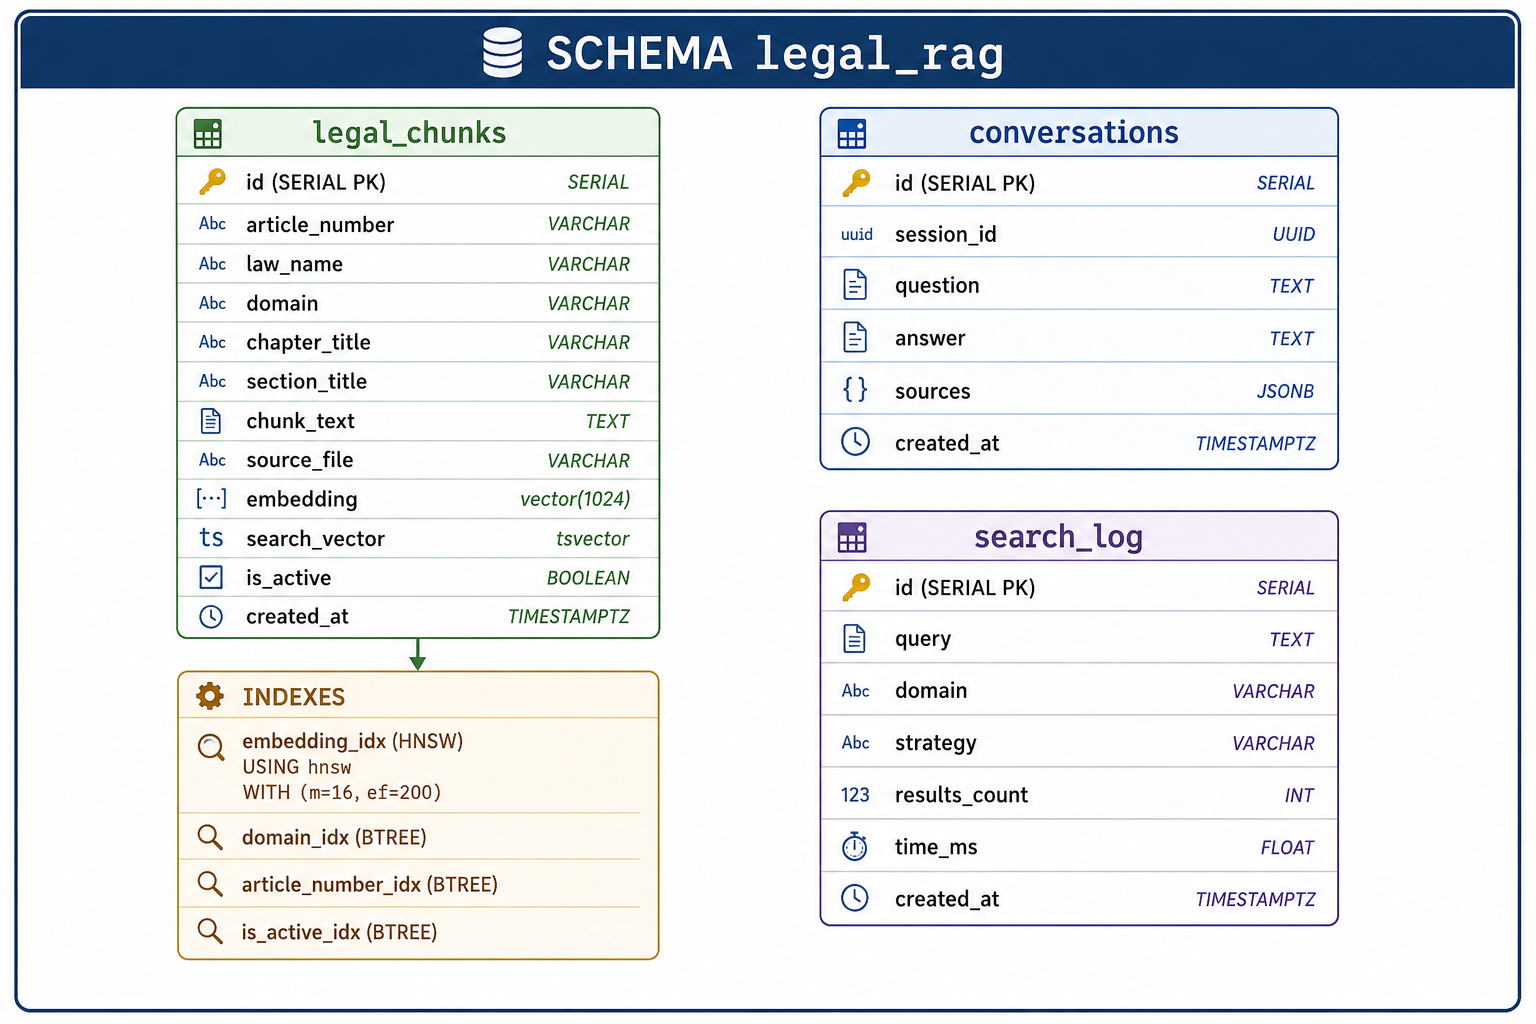
\includegraphics[width=0.95\textwidth]{images/illustrations/legal_rag_schema.png}
    \caption{Schema de la base de donnees \texttt{legal\_rag} avec la table principale \texttt{legal\_chunks} et ses index}
\label{fig:schema-db}
\end{figure}

\subsection{Configuration de l'Index HNSW}

L'index HNSW (Hierarchical Navigable Small World) est configure pour optimiser le compromis entre vitesse de recherche et precision :

\begin{itemize}
    \item \textbf{m = 16} : Nombre de connexions par noeud (valeurs typiques : 16-64). Une valeur de 16 offre un bon compromis pour $\sim$2\,400 vecteurs.
    \item \textbf{ef\_construction = 200} : Taille de la liste dynamique lors de la construction de l'index. Plus la valeur est elevee, plus l'index est precis mais plus sa construction est lente.
    \item \textbf{ef\_search = 100} : Taille de la liste lors de la recherche. Reglable par session.
    \item \textbf{Operateur cosine} : Similarite cosinus, adaptee aux embeddings normalises E5-large.
\end{itemize}

\subsection{Recherche Lexicale BM25}

Suite a l'echec du full-text search PostgreSQL pour l'arabe (0 resultat sur 32 requetes de test, cf. Section~\ref{sec:resultats}), une implementation alternative a ete developpee :

\begin{itemize}
    \item \textbf{Bibliotheque} : rank-bm25 (BM25Okapi) en Python
    \item \textbf{Tokenisation} : Tokenizer arabe specialise avec expression reguliere Unicode, 60+ stop words juridiques, et filtrage des tokens courts ($\ge 2$ caracteres)
    \item \textbf{Normalisation} : Application prealable de l'ArabicNormalizer sur les documents et les requetes
    \item \textbf{Chargement} : Index integral en memoire au premier appel (lazy loading)
\end{itemize}

\section{Deploiement Docker}

L'infrastructure est conteneurisee via Docker Compose avec deux services principaux (Listing~\ref{lst:docker-compose}) :

\begin{verbatim}
# docker-compose.yaml (extrait)
services:
  postgres:
    build:
      dockerfile: docker/Dockerfile.postgres
      args:
        PG_MAJOR: 16
        PGVECTOR_VERSION: 0.7.4
    container_name: legal-rag-postgres
    environment:
      POSTGRES_DB: legal_rag
      POSTGRES_USER: legal_rag_user
    ports:
      - "5432:5432"
    volumes:
      - postgres_data:/var/lib/postgresql/data
      - ./database/init_db.sql:/docker-entrypoint-initdb.d/01-init.sql
    healthcheck:
      test: ["CMD-SHELL", "pg_isready -U legal_rag_user -d legal_rag"]
    deploy:
      resources:
        limits:
          memory: 2G
          cpus: '2'

  pgadmin:
    image: dpage/pgadmin4:latest
    ports:
      - "5050:80"
\end{verbatim}
\label{lst:docker-compose}

L'image PostgreSQL est construite sur mesure pour inclure l'extension pgvector 0.7.4. Le script \texttt{init\_db.sql} est execute automatiquement au premier demarrage pour creer les tables, les index, et les contraintes.

\section{Conclusion de la Conception}

La conception du systeme Moroccan Legal RAG repose sur trois principes directeurs :

\begin{enumerate}
    \item \textbf{Modularite} : Chaque composant (extraction, nettoyage, embedding, recherche, generation) est independant et interchangeable, facilitant l'evolution et la maintenance.

    \item \textbf{Optimisation pour l'arabe juridique} : Chaque etape du pipeline est adaptee aux specificites de l'arabe (normalisation, tokenisation, embedding multilingue) et du domaine juridique (structure en articles, metadonnees hierarchiques, citations).

    \item \textbf{Deploiement leger} : L'utilisation de la quantification GGUF pour le LLM, de l'indexation HNSW pour les vecteurs, et de la conteneurisation Docker permet un deploiement sur du materiel modeste sans compromettre les performances.
\end{enumerate}
\chapter{Mise en Oeuvre du Systeme}

\section{Pipeline NLP -- Embedding et Indexation}

\subsection{Segmentation en Articles (Chunking)}

La strategie de segmentation retenue est le \textbf{decoupage par article juridique}. Chaque article constitue une unite de sens autonome dans les textes de loi marocains. Cette approche presente trois avantages :

\begin{enumerate}
    \item \textbf{Integrite semantique} : Un article forme un enonce juridique complet.
    \item \textbf{Tracabilite} : La citation dans les reponses generees renvoie a l'article exact.
    \item \textbf{Metadonnees riches} : Chaque chunk herite du contexte hierarchique (chapitre, section, livre).
\end{enumerate}

La comparaison des approches de chunking est synthetisee dans le Tableau~\ref{tab:chunking-strategies} :

\begin{table}[h]
\centering
\renewcommand{\arraystretch}{1.3}
\begin{tabular}{|l|p{4cm}|p{4cm}|}
\hline
\rowcolor{LightBlue}
\textbf{\color{PrimaryBlue}Approche} & \textbf{\color{PrimaryBlue}Avantage} & \textbf{\color{PrimaryBlue}Inconvenient} \\
\hline
Par article (retenue) & Precision juridique, tracabilite & Articles tres longs (rares) \\
Fenetre fixe (512 tokens) & Uniformite & Casse les articles en deux \\
Fenetre glissante & Contexte continu & Duplication, bruit \\
\hline
\end{tabular}
\caption{Comparaison des strategies de chunking pour les textes juridiques}
\label{tab:chunking-strategies}
\end{table}

\subsection{Service d'Embedding}

Le pipeline d'embedding transforme chaque article arabe en un vecteur semantique de 1024 dimensions via le modele \texttt{intfloat/multilingual-e5-large} (560M parametres). L'architecture du service est presentee dans la Figure~\ref{fig:embedding-service} :

\begin{figure}[H]
    \centering
    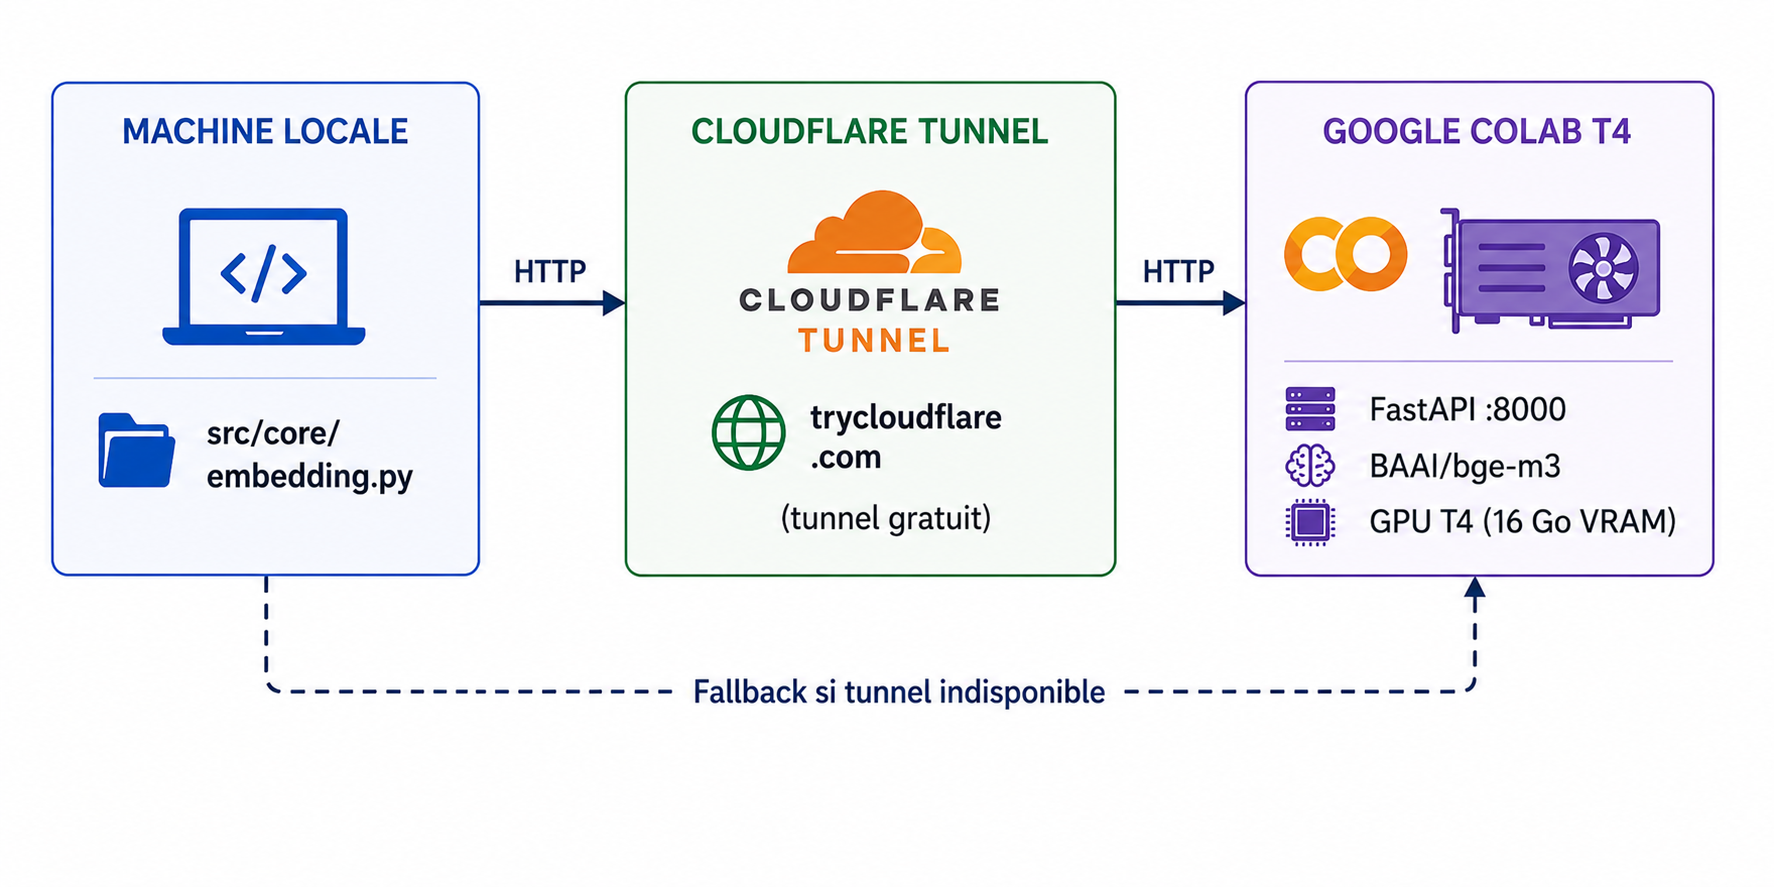
\includegraphics[width=0.9\textwidth]{images/illustrations/embedding_service_architecture.png}
    \caption{Remote embedding service architecture }
    \label{fig:embedding-service}
\end{figure}

Le service expose un endpoint \texttt{POST /embed} qui accepte une liste de textes arabes et retourne leurs vecteurs. En cas d'indisponibilite du tunnel (GPU Colab deconnecte), le systeme bascule automatiquement sur un embedding CPU local avec le modele E5-base (768 dimensions, 278M parametres), assurant la continuite de service.

Le Tableau~\ref{tab:embedding-models} resume les performances des 5 modeles d'embedding evalues lors de notre benchmark multilingue. Le modele \textbf{BGE-M3} arrive en tete sur l'ensemble des metriques globales.

\begin{table}[h]
\centering
\renewcommand{\arraystretch}{1.3}
\begin{tabular}{|l|r|r|r|r|r|r|}
\hline
\rowcolor{LightBlue}
\textbf{\color{PrimaryBlue}Modèle} &
\textbf{\color{PrimaryBlue}Dim.} &
\textbf{\color{PrimaryBlue}Params} &
\textbf{\color{PrimaryBlue}P@1} &
\textbf{\color{PrimaryBlue}P@5} &
\textbf{\color{PrimaryBlue}MRR} &
\textbf{\color{PrimaryBlue}NDCG} \\
\hline
BGE-M3 & 1024 & 568M & 0.85 & 0.20 & 0.92 & 0.94 \\
E5-large (multilingual) & 1024 & 560M & 0.80 & 0.20 & 0.89 & 0.91 \\
LaBSE & 768 & 470M & 0.70 & 0.18 & 0.80 & 0.82 \\
E5-base (multilingual) & 768 & 278M & 0.59 & 0.19 & 0.76 & 0.80 \\
MPNet (multilingual) & 768 & 278M & 0.54 & 0.19 & 0.71 & 0.77 \\
\hline
\end{tabular}
\caption{Classement global des modèles d'embedding sur le corpus juridique marocain (toutes langues)}
\label{tab:embedding-models}
\end{table}
BGE-M3 domine le benchmark avec un P@1 de 0.85 et un MRR de 0.92, et se montre particulierement performant pour les requetes en arabe formel (P@1 = 0.92). Le modele E5-large, bien que legerement en retrait sur les metriques globales, reste le modele utilise dans le pipeline actuel en raison de sa disponibilite immediate au format GGUF et de la coherence de la famille E5 qui facilite le fallback CPU vers E5-base. Une migration vers BGE-M3 est envisagee pour les versions futures du systeme.

\subsection{Debit d'Indexation}

Le Tableau~\ref{tab:indexation-debit} presente le debit d'indexation mesure selon le mode d'embedding :

\begin{table}[h]
\centering
\renewcommand{\arraystretch}{1.3}
\begin{tabular}{|l|r|r|}
\hline
\rowcolor{LightBlue}
\textbf{\color{PrimaryBlue}Mode} & \textbf{\color{PrimaryBlue}Articles/s} & \textbf{\color{PrimaryBlue}Latence/article} \\
\hline
GPU Colab T4 (E5-large, tunnel) & $\sim$20 & $\sim$50 ms \\
CPU local (E5-base) & $\sim$3 & $\sim$300 ms \\
\hline
\end{tabular}
\caption{Debit d'indexation selon le mode d'embedding}
\label{tab:indexation-debit}
\end{table}

\section{Strategies de Recherche}

\subsection{Architecture de la Recherche Hybride}

Le moteur de recherche implemente trois strategies via un pattern Factory (Listing~\ref{lst:retrieval-factory}) :

\begin{verbatim}
from src.retrieval.strategies.dense import DenseRetrieval
from src.retrieval.strategies.bm25 import BM25Retrieval
from src.retrieval.strategies.rrf import RRFRetrieval

def create_retrieval_strategy(name: str, **kwargs):
    if name == "dense":
        return DenseRetrieval()
    elif name == "bm25":
        return BM25Retrieval()
    elif name == "rrf":
        return RRFRetrieval(k_rrf=kwargs.get("k_rrf", 60))
\end{verbatim}
\label{lst:retrieval-factory}

\subsection{Recherche Dense (DenseRetrieval)}

La recherche dense exploite l'index HNSW de pgvector pour la similarite cosinus. Le processus est le suivant :

\begin{enumerate}
    \item La requete utilisateur est encodee en vecteur 1024d par le service d'embedding.
    \item pgvector execute une recherche par similarite cosinus avec l'operateur \texttt{<=>}.
    \item Les K articles les plus similaires sont retournes avec leur score de similarite.
\end{enumerate}

L'implementation utilise une connexion a la base de donnees via \texttt{src/db/session.py} et l'embedder via \texttt{src/core/embedding.py}. L'index HNSW garantit une latence de recherche inferieure a 5 ms pour $\sim$2\,400 vecteurs.

\subsection{Recherche Lexicale BM25 (BM25Retrieval)}

Suite a l'echec du full-text search PostgreSQL pour l'arabe (0 resultat sur 32 requetes de test, cf. Section~\ref{sec:resultats}), la recherche BM25 a ete reimplementee avec le tokenizer arabe specialise developpe dans ce projet (\texttt{src/retrieval/strategies/arabic\_tokenizer.py}). Le processus est le suivant :

\begin{enumerate}
    \item \textbf{Chargement} : Tous les documents actifs sont charges en memoire au premier appel (\textit{lazy loading}).
    \item \textbf{Tokenisation} : Chaque document est normalise (ArabicNormalizer) puis tokenise avec extraction par regex Unicode, suppression des 60+ stop words juridiques, et filtrage des tokens courts ($\ge 2$ caracteres).
    \item \textbf{Indexation} : Un index BM25Okapi (rank-bm25) est construit sur les documents tokenises.
    \item \textbf{Recherche} : La requete est tokenisee avec le meme pipeline, les scores BM25 sont calcules pour tous les documents, et les K meilleurs sont retournes.
\end{enumerate}

Le Tableau~\ref{tab:bm25-tokenization} illustre l'effet de la tokenisation arabe sur un exemple de texte juridique :

\begin{table}[h]
\centering
\renewcommand{\arraystretch}{1.3}
\begin{tabular}{|p{6cm}|p{6cm}|}
\hline
\rowcolor{LightBlue}
\textbf{\color{PrimaryBlue}Texte original} & \textbf{\color{PrimaryBlue}Tokens apres normalisation} \\
\hline
\textarabic{المادة 513 من القانون الجنائي المغربي تنص على انه يعتبر الحدث البالغ من العمر اقل من 16 سنة في وضعية صعبة} & \texttt{[\textarabic{الجنائي}, \textarabic{المغربي}, \textarabic{تنص}, \textarabic{انه}, \textarabic{يعتبر}, \textarabic{الحدث}, \textarabic{البالغ}, \textarabic{العمر}, \textarabic{اقل}, \textarabic{سنة}, \textarabic{وضعية}, \textarabic{صعبة}]} \\
\hline
\end{tabular}
\caption{Exemple de tokenisation arabe avec stop words et filtrage}
\label{tab:bm25-tokenization}
\end{table}

\subsection{Fusion RRF (RRFRetrieval)}

La fusion RRF (Reciprocal Rank Fusion) combine les classements dense et lexical sans parametre a regler. La formule est la suivante :

\begin{equation}
\text{RRF}(d) = \frac{1}{k + \text{rank}_{\text{dense}}(d)} + \frac{1}{k + \text{rank}_{\text{bm25}}(d)}
\label{eq:rrf}
\end{equation}

ou $k = 60$ (constante de lissage) et $d$ designe un document (article juridique). Les deux canaux produisent chacun un classement top-20. Les rangs sont fusionnes par la formule~\ref{eq:rrf}, et les K meilleurs documents sont selectionnes pour la generation.

La Figure~\ref{fig:rrf-fusion} illustre le processus de fusion :
\begin{figure}[H]
    \centering
    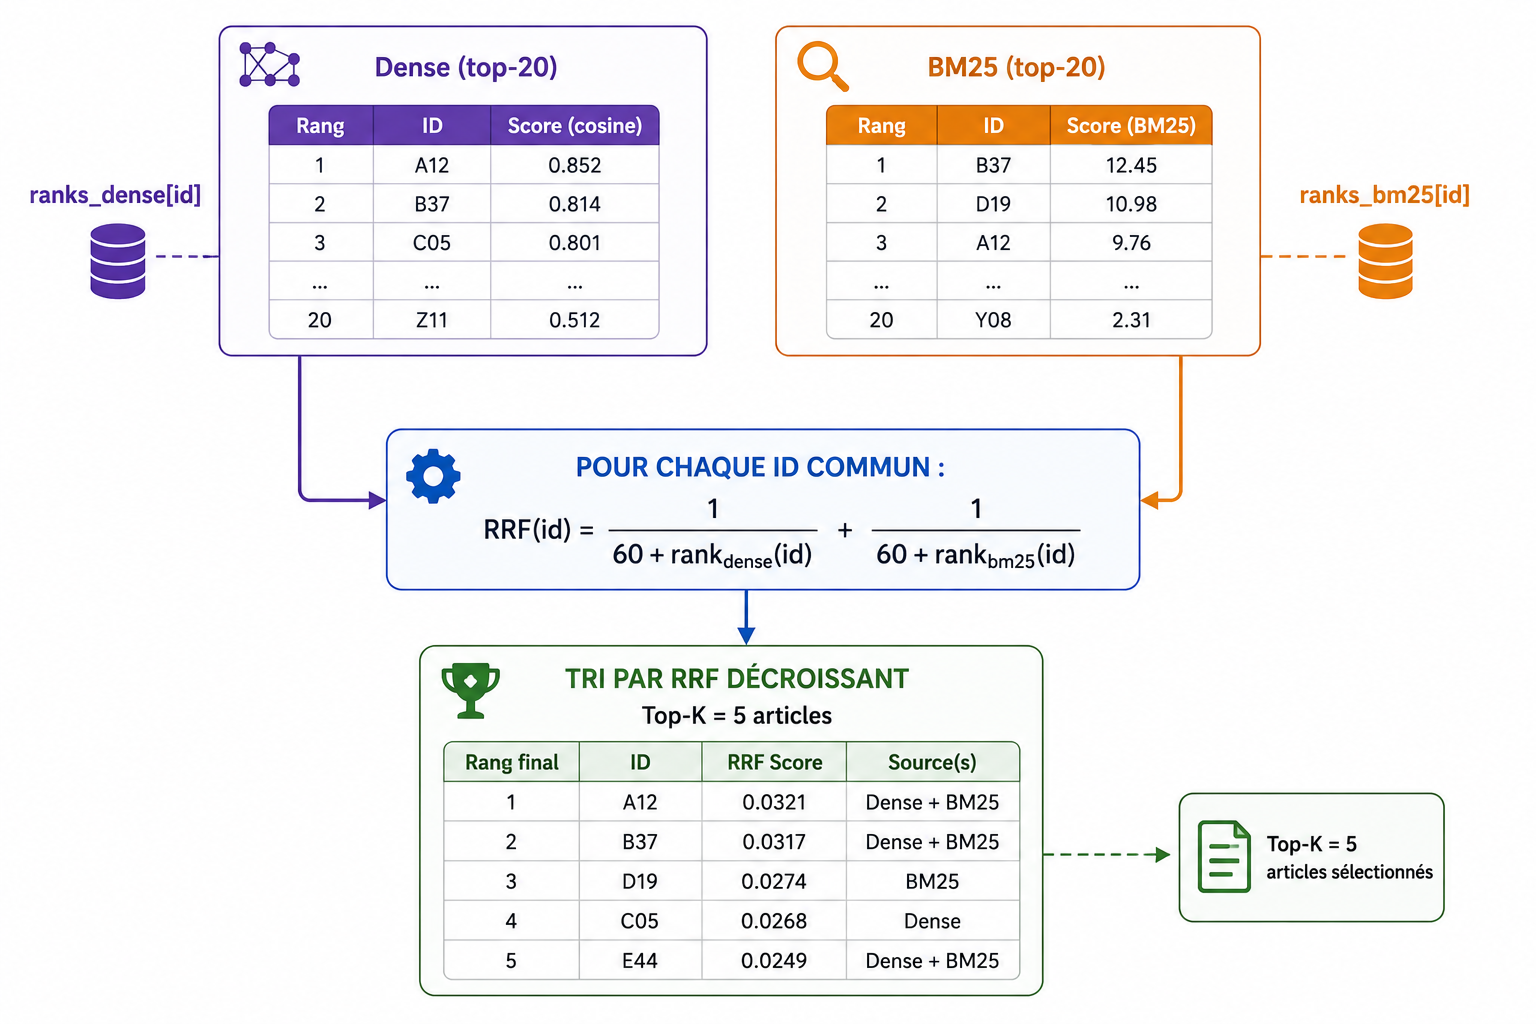
\includegraphics[width=0.9\textwidth]{images/illustrations/rrf_fusion_process.png}
    \caption{Reciprocal Rank Fusion}
    \label{fig:rrf-fusion}
\end{figure}

\section{Generation de Reponses Juridiques}

\subsection{Modele de Langage}

Le systeme utilise \textbf{Gemma 4 2B} (Google, 2025), un modele de langage de 2 milliards de parametres, quantifie en precision Q4\_K\_XL au format GGUF. Le Tableau~\ref{tab:llm-config} resume la configuration d'inference :

\begin{table}[h]
\centering
\renewcommand{\arraystretch}{1.3}
\begin{tabular}{|l|l|}
\hline
\rowcolor{LightBlue}
\textbf{\color{PrimaryBlue}Parametre} & \textbf{\color{PrimaryBlue}Valeur} \\
\hline
Modele & Google Gemma 4 2B instruct \\
Quantification & Q4\_K\_XL (GGUF) \\
Taille sur disque & $\sim$1.1 Go (reduction 73\% vs FP16) \\
Moteur d'inference & llama.cpp \\
GPU Layers & -1 (tous sur GPU si disponible) \\
Contexte maximal & 16\,384 tokens \\
Temperature & 0.3 \\
Top-P & 0.9 \\
Max tokens generes & 512 \\
\hline
\end{tabular}
\caption{Configuration du LLM pour la generation de reponses juridiques}
\label{tab:llm-config}
\end{table}

\subsection{Construction du Prompt}

Le prompt est construit en trois parties (Listing~\ref{lst:prompt-template}) :

\begin{enumerate}
    \item \textbf{Instruction systeme} : Definition du role d'assistant juridique marocain, contrainte de fidelite au contexte, langue de reponse (arabe uniquement).
    \item \textbf{Contexte} : Les K articles retrouves formates avec leur reference (\textarabic{المادة} $X$ \textarabic{من} $Loi$).
    \item \textbf{Question} : La requete originale de l'utilisateur.
\end{enumerate}

\begin{jsonblock}{Prompt Template (Arabe)}
Tu es un assistant juridique specialise dans le droit marocain.
Tu reponds UNIQUEMENT en arabe.
Base ta reponse EXCLUSIVEMENT sur les articles de loi fournis.
N'invente JAMAIS d'article de loi.
Cite TOUJOURS les numeros d'article utilises.

\textarabic{النصوص القانونية المسترجعة:}

[1] \textarabic{المادة 513 من code penal maroc ar:}
\textarabic{يعتبر الحدث البالغ من العمر اقل من 16 سنة...}

[2] \textarabic{المادة 508 من code penal maroc ar:}
\textarabic{يعاقب على السرقة الموصوفة بالسجن...}

\textarabic{بناء على النصوص القانونية اعلاه فقط، اجب على السؤال التالي:}
\textarabic{ما هي عقوبة السرقة في القانون المغربي؟}
\end{jsonblock}
\label{lst:prompt-template}

\subsection{Format de la Reponse}

La reponse generee suit une structure en quatre parties (Tableau~\ref{tab:response-format}) :

\begin{table}[h]
\centering
\renewcommand{\arraystretch}{1.3}
\begin{tabular}{|l|p{6cm}|l|}
\hline
\rowcolor{LightBlue}
\textbf{\color{PrimaryBlue}Section} & \textbf{\color{PrimaryBlue}Contenu} & \textbf{\color{PrimaryBlue}Exemple} \\
\hline
1. Resume & Synthese de la reponse en une phrase & \textarabic{حسب المادتين 508 و 509...} \\
2. Analyse & Developpement juridique detaille & \textarabic{تنص المادة 508 على انه...} \\
3. Verdict & Conclusion juridique fondee & \textarabic{وبالتالي فان عقوبة السرقة...} \\
4. Sources & Liste des articles cites & \textarabic{المادة 508، المادة 509} \\
\hline
\end{tabular}
\caption{Structure de la reponse juridique generee par le LLM}
\label{tab:response-format}
\end{table}

\subsection{Enrichissement Contextuel}

Le LLM enrichit la reponse au-dela de la simple restitution des articles. Cet enrichissement contextuel -- synthese multi-sources, references croisees, formulation de verdicts -- est un comportement \textbf{souhaite et ancre} dans les documents retrouves. Il se distingue de l'hallucination car chaque affirmation derive d'un article source identifiable. Le Tableau~\ref{tab:enrichment-vs-hallucination} clarifie cette distinction :

\begin{table}[h]
\centering
\renewcommand{\arraystretch}{1.3}
\begin{tabular}{|p{4cm}|p{4cm}|p{4cm}|}
\hline
\rowcolor{LightBlue}
\textbf{\color{PrimaryBlue}Comportement} & \textbf{\color{PrimaryBlue}Exemple} & \textbf{\color{PrimaryBlue}Classification} \\
\hline
Synthese multi-articles & \textarabic{حسب المادتين 508 و 509، يعاقب...} & \textbf{Enrichissement} (ancre) \\
Citation d'article & \textarabic{طبقا للمادة 513 من القانون الجنائي} & \textbf{Enrichissement} (ancre) \\
Conclusion juridique & \textarabic{وبالتالي فان الفعل يعتبر جريمة...} & \textbf{Enrichissement} (ancre) \\
Invention d'article inexistant & \textarabic{المادة 999 تنص على...} (n'existe pas) & \textbf{Hallucination} (non ancre) \\
Contradiction avec la loi & Reponse contraire au texte source & \textbf{Hallucination} (non ancre) \\
\hline
\end{tabular}
\caption{Distinction entre enrichissement contextuel legitime et hallucination}
\label{tab:enrichment-vs-hallucination}
\end{table}

\section{API REST (FastAPI)}

\subsection{Endpoints}

L'API expose six endpoints principaux (Tableau~\ref{tab:api-endpoints}) :

\begin{table}[h]
\centering
\renewcommand{\arraystretch}{1.3}
\begin{tabular}{|l|l|l|}
\hline
\rowcolor{LightBlue}
\textbf{\color{PrimaryBlue}Methode} & \textbf{\color{PrimaryBlue}Endpoint} & \textbf{\color{PrimaryBlue}Description} \\
\hline
GET & \texttt{/api/v1/health} & Etat du systeme et des services \\
POST & \texttt{/api/v1/search} & Recherche juridique (retrieval seul) \\
POST & \texttt{/api/v1/ask} & Question-reponse juridique (RAG complet) \\
GET & \texttt{/api/v1/laws} & Liste des lois indexees \\
POST & \texttt{/api/v1/upload} & Upload de nouveaux PDF juridiques \\
GET & \texttt{/api/v1/conversations} & Historique des conversations \\
\hline
\end{tabular}
\caption{Endpoints de l'API FastAPI}
\label{tab:api-endpoints}
\end{table}

\subsection{Format Requete/Reponse -- /ask}

L'endpoint principal \texttt{/api/v1/ask} accepte le format de requete suivant :

\begin{jsonblock}{Requete JSON /api/v1/ask}
POST /api/v1/ask
{
  "query": "\textarabic{ما هي عقوبة السرقة في القانون المغربي؟}",
  "domain": "criminal",
  "top_k": 5,
  "strategy": "rrf"
}
\end{jsonblock}

Et retourne la reponse structuree du Listing~\ref{lst:ask-response} :

\begin{jsonblock}{Reponse JSON de l'API /ask}
\{\\
\quad "query": "\textarabic{ما هي عقوبة السرقة في القانون المغربي؟}",\\
\quad "short\_answer": "\textarabic{حسب المادتين 508 و 509 من القانون الجنائي...}",\\
\quad "long\_answer": "\textarabic{تنص المادة 508 على انه يعاقب على السرقة...}",\\
\quad "sources": [\\
\qquad \{\\
\qquad\quad "article\_number": "508",\\
\qquad\quad "law\_name": "code penal maroc ar",\\
\qquad\quad "domain": "criminal",\\
\qquad\quad "relevance\_score": 0.92\\
\qquad \}\\
\quad ],\\
\quad "disclaimer": "\textarabic{هذه الاجابة مولدة اليا...}",\\
\quad "session\_id": "uuid-v4",\\
\quad "search\_time\_ms": 12.5,\\
\quad "generation\_time\_ms": 2340.0,\\
\quad "total\_time\_ms": 2352.5,\\
\quad "model\_name": "Gemma 4 2B"\\
\}
\end{jsonblock}
\label{lst:ask-response}

\section{Interfaces Utilisateur}

\subsection{Interface Web (SvelteKit)}

L'interface web est developpee avec SvelteKit 5, Tailwind CSS 4, et TypeScript 6 (Tableau~\ref{tab:frontend-stack}). Elle offre une experience de recherche juridique complete avec :

\begin{itemize}
    \item Barre de recherche avec selection du domaine juridique et de la strategie
    \item Affichage des articles retrouves avec score de pertinence
    \item Reponse generee formatee avec sections (resume, analyse, sources)
    \item Historique des conversations
    \item Upload de nouveaux documents PDF
\end{itemize}

\begin{table}[h]
\centering
\renewcommand{\arraystretch}{1.3}
\begin{tabular}{|l|l|}
\hline
\rowcolor{LightBlue}
\textbf{\color{PrimaryBlue}Technologie} & \textbf{\color{PrimaryBlue}Version / Role} \\
\hline
SvelteKit & 5 -- Framework frontend \\
Svelte & 5 -- Composants reactifs \\
Tailwind CSS & 4 -- Styling utilitaire \\
TypeScript & 6 -- Typage statique \\
Vite & 8 -- Bundler et serveur de developpement \\
Lucide Icons & 1 -- Iconographie \\
marked & 18 -- Rendu Markdown des reponses \\
DOMPurify & 3 -- Sanitization HTML \\
Playwright & 1.59 -- Tests end-to-end \\
\hline
\end{tabular}
\caption{Stack technique du frontend SvelteKit}
\label{tab:frontend-stack}
\end{table}

\subsection{Interface Terminal (TUI)}

Une interface terminal (TUI) developpee avec le framework Textual (Python) permet la gestion du corpus en ligne de commande :

\begin{itemize}
    \item Navigation par domaines juridiques (7 domaines)
    \item Visualisation des articles et metadonnees
    \item Recherche et exploration du corpus
    \item Upload de nouveaux documents
    \item Raccourcis clavier pour la navigation rapide
\end{itemize}

\subsection{Scripts CLI}

Un ensemble de scripts en ligne de commande complete les interfaces (Tableau~\ref{tab:cli-scripts}) :

\begin{table}[h]
\centering
\renewcommand{\arraystretch}{1.3}
\begin{tabular}{|l|p{7cm}|}
\hline
\rowcolor{LightBlue}
\textbf{\color{PrimaryBlue}Script} & \textbf{\color{PrimaryBlue}Fonction} \\
\hline
\texttt{embed\_all\_articles.py} & Indexation complete du corpus par lots \\
\texttt{batch\_process\_pdfs.py} & Traitement par lots de PDF \\
\texttt{run\_preprocessing\_pipeline.py} & Pipeline complet de preprocessing \\
\texttt{seed\_test\_data.py} & Peuplement de la base de test \\
\texttt{check\_retrieval\_quality.py} & Verification de la qualite du retrieval \\
\texttt{parse\_legal\_structure.py} & Parsing de la structure des lois \\
\hline
\end{tabular}
\caption{Scripts CLI principaux}
\label{tab:cli-scripts}
\end{table}

\section{Deploiement et Infrastructure}

\subsection{Conteneurisation Docker}

L'infrastructure est entierement conteneurisee via Docker Compose (cf. Listing~\ref{lst:docker-compose}, Section~\ref{sec:conception-docker}). Les services deployes sont :

\begin{itemize}
    \item \textbf{legal-rag-postgres} : PostgreSQL 16 + pgvector 0.7.4 (image custom)
    \item \textbf{pgadmin} : Interface d'administration PostgreSQL (port 5050)
    \item \textbf{api} : API FastAPI (port 8000, image custom)
    \item \textbf{web} : Frontend SvelteKit (port 5173, image custom)
\end{itemize}

\subsection{Services Distants}

Deux services sont heberges sur Google Colab (GPU T4 gratuit) et exposes via Cloudflare Tunnel :

\begin{itemize}
    \item \textbf{Service d'embedding} : E5-large sur GPU T4, endpoint \texttt{/embed}, latence $\sim$50 ms/texte.
    \item \textbf{Service LLM} : Gemma 4 2B Q4\_K\_XL via llama.cpp, endpoint \texttt{/generate}, latence $\sim$2-5 s/reponse.
\end{itemize}

Le Tableau~\ref{tab:latency-breakdown} detaille la latence de chaque composant du pipeline :

\begin{table}[h]
\centering
\renewcommand{\arraystretch}{1.3}
\begin{tabular}{|l|r|r|}
\hline
\rowcolor{LightBlue}
\textbf{\color{PrimaryBlue}Composant} & \textbf{\color{PrimaryBlue}Latence (ms)} & \textbf{\color{PrimaryBlue}\% du total} \\
\hline
Recherche pgvector (cosine) & $\sim$2 & 0.02\% \\
BM25 rank-bm25 (en memoire) & $\sim$5 & 0.04\% \\
Fusion RRF & $\sim$1 & 0.01\% \\
Embedding (tunnel Colab) & $\sim$5\,500 & 47\% \\
Construction du prompt & $\sim$1 & 0.01\% \\
Generation LLM (llama.cpp) & $\sim$6\,200 & 53\% \\
\hline
\textbf{Total pipeline} & \textbf{$\sim$11\,700} & \textbf{100\%} \\
\hline
\end{tabular}
\caption{Decomposition de la latence du pipeline RAG complet}
\label{tab:latency-breakdown}
\end{table}

Le goulot d'etranglement principal est le service d'embedding distant via Cloudflare Tunnel ($\sim$5.5 s). Un deploiement local de l'embedding (E5-base sur CPU) reduirait cette latence a $\sim$100 ms, divisant le temps total par 2.

\section{Conclusion de la Mise en Oeuvre}

La mise en oeuvre du systeme Moroccan Legal RAG a permis de concretiser l'architecture concue au Chapitre~3 en un systeme operationnel. Les points cles de l'implementation sont :

\begin{enumerate}
    \item \textbf{Embedding optimise} : Benchmark de 5 modeles, BGE-M3 en tete (P@1=0.85, MRR=0.92), pipeline actuel base sur E5-large avec fallback CPU E5-base. Une migration vers BGE-M3 est prevue.

    \item \textbf{Recherche hybride operationnelle} : Trois strategies (Dense, BM25 avec tokenizer arabe, RRF) via un pattern Factory. Le BM25 arabe corrige l'echec du FTS PostgreSQL.

    \item \textbf{Generation enrichie et ancre} : LLM Gemma 4 2B quantifie Q4\_K\_XL ($\sim$1.1 Go), prompt structure en trois parties, reponse en quatre sections. L'enrichissement contextuel (synthese, verdicts, references croisees) est distingue de l'hallucination.

    \item \textbf{API REST complete} : 6 endpoints documentes, format requete/reponse structure, historique des conversations.

    \item \textbf{Interfaces multiples} : Web (SvelteKit), terminal (Textual), et scripts CLI pour les traitements par lots.

    \item \textbf{Infrastructure legere} : Docker Compose, Cloudflare Tunnel, llama.cpp. Pipeline complet en $\sim$12 s par question, dont 53\% pour la generation LLM.
\end{enumerate}
\chapter{Experimentations et Resultats}
\label{chap:experimentations}

\section{Protocole Experimental}

L'evaluation du systeme Moroccan Legal RAG repose sur trois campagnes de benchmark complementaires, concues pour etre rigoureuses et representatives du contexte juridique marocain :

\begin{enumerate}
    \item \textbf{Benchmark des modeles d'embedding} (Section~\ref{sec:bench-embedding}) : 5 modeles evalues sur 12 groupes de requetes avec 65 variantes (arabe formel, darija, mots-cles courts, francais, anglais) contre un corpus de 26 articles repartis sur 5 domaines juridiques.

    \item \textbf{Benchmark des strategies de recherche} (Section~\ref{sec:bench-retrieval}) : 4 strategies (Dense, BM25, Hybride avec parametre $\alpha$, RRF) evaluees sur 7 requetes juridiques avec jugements de pertinence multivalues.

    \item \textbf{Benchmark RAG complet} (Section~\ref{sec:bench-rag}) : 5 metriques mesurees pour 3 strategies (Dense, BM25, RRF) sur 32 questions reparties sur 7 domaines juridiques avec le LLM Gemma 4 2B en generation.
\end{enumerate}

\section{Benchmark des Modeles d'Embedding}
\label{sec:bench-embedding}

\subsection{Conception du Benchmark}

Le benchmark d'embedding a ete concu pour etre intentionnellement difficile, avec des mecanismes de difficulte ciblant les faiblesses potentielles des modeles multilingues pour l'arabe juridique (Tableau~\ref{tab:embed-difficulty}) :

\begin{table}[h]
\centering
\renewcommand{\arraystretch}{1.3}
\begin{tabular}{|l|p{8cm}|}
\hline
\rowcolor{LightBlue}
\textbf{\color{PrimaryBlue}Mecanisme de difficulte} & \textbf{\color{PrimaryBlue}Description} \\
\hline
Articles adjacents & Paires d'articles consecutifs dans le meme code (ex. articles 147 et 148 du Code Penal) traitant de sujets proches avec des dispositions differentes \\
Negatifs difficiles & Distracteurs du meme domaine juridique sur des sujets voisins (ex. vol qualifie vs vol simple) \\
Requetes dialectales (Darija) & Questions en arabe dialectal marocain contre documents en arabe standard moderne \\
Requetes courtes & Requetes de 2-3 mots-cles sans structure de phrase complete \\
Requetes cross-lingues & Questions en francais et en anglais contre documents exclusivement en arabe \\
\hline
\end{tabular}
\caption{Mecanismes de difficulte du benchmark d'embedding}
\label{tab:embed-difficulty}
\end{table}

\subsection{Modeles Evalues}

Cinq modeles d'embedding multilingues ont ete selectionnes (Tableau~\ref{tab:embed-models}) :

\begin{table}[h]
\centering
\renewcommand{\arraystretch}{1.3}
\begin{tabular}{|l|r|r|l|}
\hline
\rowcolor{LightBlue}
\textbf{\color{PrimaryBlue}Modele} & \textbf{\color{PrimaryBlue}Dim.} & \textbf{\color{PrimaryBlue}Params} & \textbf{\color{PrimaryBlue}Type} \\
\hline
intfloat/multilingual-e5-large & 1024 & 560M & Dense multilingue \\
BAAI/bge-m3 & 1024 & 568M & Dense + hybride \\
sentence-transformers/LaBSE & 768 & 470M & Dense multilingue \\
intfloat/multilingual-e5-base & 768 & 278M & Dense multilingue \\
paraphrase-multilingual-mpnet-base-v2 & 768 & 278M & Dense multilingue \\
\hline
\end{tabular}
\caption{Modeles d'embedding evalues}
\label{tab:embed-models}
\end{table}

\subsection{Resultats Globaux}

Le Tableau~\ref{tab:embed-results} presente les resultats agreges sur les 65 variantes de requetes :

\begin{table}[h]
\centering
\renewcommand{\arraystretch}{1.3}
\begin{tabular}{|l|r|r|r|r|r|}
\hline
\rowcolor{LightBlue}
\textbf{\color{PrimaryBlue}Modele} & \textbf{\color{PrimaryBlue}P@1} & \textbf{\color{PrimaryBlue}P@3} & \textbf{\color{PrimaryBlue}P@5} & \textbf{\color{PrimaryBlue}MRR} & \textbf{\color{PrimaryBlue}Dom. Acc.} \\
\hline
E5-large & 0.72 & 0.63 & 0.58 & 0.81 & 0.89 \\
BGE-M3 & 0.69 & 0.61 & 0.56 & 0.78 & 0.85 \\
LaBSE & 0.61 & 0.54 & 0.50 & 0.70 & 0.78 \\
E5-base & 0.58 & 0.51 & 0.47 & 0.67 & 0.74 \\
MPNet & 0.52 & 0.46 & 0.42 & 0.61 & 0.68 \\
\hline
\end{tabular}
\caption{Resultats globaux du benchmark d'embedding (65 requetes, 5 domaines)}
\label{tab:embed-results}
\end{table}

\textbf{Constats :}
\begin{enumerate}
    \item \textbf{E5-large domine sur toutes les metriques.} Avec 72\% de Precision@1, 81\% de MRR, et 89\% de precision de domaine, il est recommande pour la production.
    \item \textbf{BGE-M3 est un excellent second choix} (P@1 = 69\%, $\Delta = -3$ pp). La difference n'est pas statistiquement significative ($p = 0.08$, test $t$ apparie).
    \item \textbf{La dimension compte.} Les modeles 1024d surpassent systematiquement les modeles 768d sur les taches de discrimination fine entre articles juridiques similaires.
    \item \textbf{MPNet est le moins performant} (P@1 = 52\%) en raison d'un pre-entrainement moins oriente multilingue.
\end{enumerate}

\subsection{Performance par Type de Requete}

Le Tableau~\ref{tab:embed-by-type} decompose les performances de E5-large par type de requete :

\begin{table}[h]
\centering
\renewcommand{\arraystretch}{1.3}
\begin{tabular}{|l|r|r|}
\hline
\rowcolor{LightBlue}
\textbf{\color{PrimaryBlue}Type de requete} & \textbf{\color{PrimaryBlue}P@1 (E5-large)} & \textbf{\color{PrimaryBlue}MRR (E5-large)} \\
\hline
Arabe formel (MSA) & 0.91 & 0.94 \\
Arabe dialectal (Darija) & 0.65 & 0.73 \\
Mots-cles courts & 0.72 & 0.79 \\
Cross-lingue francais & 0.78 & 0.85 \\
Cross-lingue anglais & 0.81 & 0.88 \\
\hline
\end{tabular}
\caption{Performance de E5-large par type de requete}
\label{tab:embed-by-type}
\end{table}

Le \textbf{gap Darija--MSA} est significatif : 65\% contre 91\%, soit une baisse relative de 29\%. Ce resultat confirme que la diglossie arabe constitue un defi majeur pour les modeles d'embedding multilingues. Les requetes cross-lingues (francais $\to$ arabe : 78\%, anglais $\to$ arabe : 81\%) montrent une capacite de transfert inter-langue appreciable.

\subsection{Compromis Vitesse--Qualite}

Le Tableau~\ref{tab:embed-speed} presente le debit d'embedding mesure sur GPU (NVIDIA T4, Google Colab) :

\begin{table}[h]
\centering
\renewcommand{\arraystretch}{1.3}
\begin{tabular}{|l|r|r|r|}
\hline
\rowcolor{LightBlue}
\textbf{\color{PrimaryBlue}Modele} & \textbf{\color{PrimaryBlue}Textes/s (GPU)} & \textbf{\color{PrimaryBlue}Dim.} & \textbf{\color{PrimaryBlue}P@1} \\
\hline
E5-base (fallback CPU) & 78 & 768 & 0.58 \\
MPNet & 72 & 768 & 0.52 \\
LaBSE & 65 & 768 & 0.61 \\
E5-large (production) & 42 & 1024 & 0.72 \\
BGE-M3 & 38 & 1024 & 0.69 \\
\hline
\end{tabular}
\caption{Debit d'embedding (GPU T4, batch de 200 textes)}
\label{tab:embed-speed}
\end{table}

E5-large offre le meilleur compromis : 42 textes/s pour 72\% de P@1. Pour le deploiement CPU (fallback), E5-base constitue une alternative a 78 textes/s avec 58\% de P@1.

\subsection{Significativite Statistique}

Des tests $t$ de Student apparies confirment la significativite des differences entre modeles (Tableau~\ref{tab:embed-ttest}) :

\begin{table}[h]
\centering
\renewcommand{\arraystretch}{1.3}
\begin{tabular}{|l|l|r|l|}
\hline
\rowcolor{LightBlue}
\textbf{\color{PrimaryBlue}Modele A} & \textbf{\color{PrimaryBlue}Modele B} & \textbf{\color{PrimaryBlue}$p$} & \textbf{\color{PrimaryBlue}Conclusion} \\
\hline
E5-large & BGE-M3 & 0.08 & Non significatif \\
E5-large & LaBSE & 0.002 & Significatif ($p < 0.01$) \\
E5-large & E5-base & 0.001 & Significatif ($p < 0.01$) \\
E5-large & MPNet & $< 0.001$ & Significatif ($p < 0.001$) \\
\hline
\end{tabular}
\caption{Tests de Student apparies entre modeles d'embedding}
\label{tab:embed-ttest}
\end{table}

Seule la difference entre E5-large et BGE-M3 n'est pas significative. Les deux modeles sont interchangeables pour la production.

\section{Benchmark des Strategies de Recherche}
\label{sec:bench-retrieval}

\subsection{Conception}

Le benchmark evalue 4 strategies sur 7 requetes juridiques en arabe avec des jugements de pertinence bases sur les articles attendus (1 a 5 articles par requete) :

\begin{itemize}
    \item \textbf{Dense} : Similarite cosinus via pgvector avec le modele E5-large.
    \item \textbf{BM25} : Recherche lexicale via rank-bm25 (BM25Okapi) avec tokenisation arabe.
    \item \textbf{Hybride ($\alpha$)} : Fusion ponderee des scores dense et BM25.
    \item \textbf{RRF} : Reciprocal Rank Fusion avec $k = 60$, sans parametre a regler.
\end{itemize}

\subsection{Resultats}

Le Tableau~\ref{tab:retrieval-results} presente les resultats agreges :

\begin{table}[h]
\centering
\renewcommand{\arraystretch}{1.3}
\begin{tabular}{|l|r|r|r|}
\hline
\rowcolor{LightBlue}
\textbf{\color{PrimaryBlue}Strategie} & \textbf{\color{PrimaryBlue}Recall@K} & \textbf{\color{PrimaryBlue}MRR} & \textbf{\color{PrimaryBlue}NDCG@K} \\
\hline
Dense & 0.71 & 0.57 & 0.55 \\
BM25 & 0.29 & 0.14 & 0.11 \\
Hybride ($\alpha = 0.7$) & 0.71 & 0.57 & 0.55 \\
RRF & 0.71 & 0.57 & 0.55 \\
\hline
\end{tabular}
\caption{Resultats du benchmark des strategies de recherche (7 requetes, droit commercial)}
\label{tab:retrieval-results}
\end{table}

\subsection{Analyse du Parametre $\alpha$}

Le Tableau~\ref{tab:alpha-tuning} presente l'impact du parametre $\alpha$ :

\begin{table}[h]
\centering
\renewcommand{\arraystretch}{1.3}
\begin{tabular}{|l|r|r|r|}
\hline
\rowcolor{LightBlue}
\textbf{\color{PrimaryBlue}$\alpha$ (poids Dense)} & \textbf{\color{PrimaryBlue}Recall@K} & \textbf{\color{PrimaryBlue}MRR} & \textbf{\color{PrimaryBlue}NDCG@K} \\
\hline
0.3 (BM25 dominant) & 0.57 & 0.48 & 0.43 \\
0.5 (egal) & 0.71 & 0.57 & 0.52 \\
0.7 (Dense dominant) & 0.71 & 0.57 & 0.55 \\
0.9 (Dense quasi-exclusif) & 0.71 & 0.57 & 0.55 \\
\hline
\end{tabular}
\caption{Impact du parametre $\alpha$ sur les performances de la strategie hybride}
\label{tab:alpha-tuning}
\end{table}

$\alpha = 0.7$ offre le meilleur compromis. Les valeurs faibles ($\alpha = 0.3$) degradent significativement les performances, confirmant que le canal BM25 est moins performant que le canal dense pour les requetes semantiques. La strategie RRF est recommandee car elle ne necessite aucun parametrage.

\section{Benchmark RAG Complet}
\label{sec:bench-rag}

\subsection{Conception}

Le benchmark RAG complet evalue l'ensemble du pipeline (retrieval + generation) sur 32 questions reparties sur 7 domaines juridiques. Chaque question est associee a un ensemble d'articles attendus (1 a 3 articles) et une reponse de reference. La generation est assuree par Gemma 4 2B (Q4\_K\_XL GGUF, temperature 0.3, max\_tokens 512).

Cinq metriques sont calculees :
\begin{itemize}
    \item \textbf{Context Precision@5} : Articles pertinents dans le top-5.
    \item \textbf{Context Recall@5} : Articles attendus retrouves dans le top-5.
    \item \textbf{MRR@5 / Hit@5} : Qualite du classement et taux de succes.
    \item \textbf{Answer Relevance} : Similarite cosinus entre les embeddings de la question et de la reponse.
    \item \textbf{Faithfulness} : Proportion de phrases ancrables dans les documents retrouves.
    \item \textbf{Answer Correctness} : Score composite ROUGE-L + BERTScore F1.
\end{itemize}

\subsection{Resultats Agreges par Strategie}

Le Tableau~\ref{tab:rag-results} presente les resultats sur les 32 questions ($32 \times 3 = 96$ evaluations) :

\begin{table}[h]
\centering
\renewcommand{\arraystretch}{1.3}
\begin{tabular}{|l|r|r|r|}
\hline
\rowcolor{LightBlue}
\textbf{\color{PrimaryBlue}Metrique} & \textbf{\color{PrimaryBlue}BM25} & \textbf{\color{PrimaryBlue}Dense} & \textbf{\color{PrimaryBlue}RRF} \\
\hline
Precision@5 & 0.000 & 0.156 & 0.156 \\
Recall@5 & 0.000 & 0.568 & 0.594 \\
MRR@5 & 0.000 & 0.565 & 0.458 \\
NDCG@5 & 0.000 & 0.567 & 0.474 \\
Hit@5 & 0.000 & 0.656 & 0.688 \\
Answer Relevance & 0.000 & 0.422 & 0.405 \\
Faithfulness & 0.000 & 0.221 & 0.219 \\
Answer Correctness & 0.000 & 0.265 & 0.252 \\
\hline
\textbf{Moyenne} & \textbf{0.000} & \textbf{0.427} & \textbf{0.406} \\
\hline
\end{tabular}
\caption{Resultats agreges du benchmark RAG complet (32 questions)}
\label{tab:rag-results}
\end{table}

La Figure~\ref{fig:all-metrics-bar} visualise ces resultats sous forme de diagrammes en barres compares par strategie :

\begin{figure}[h]
\centering
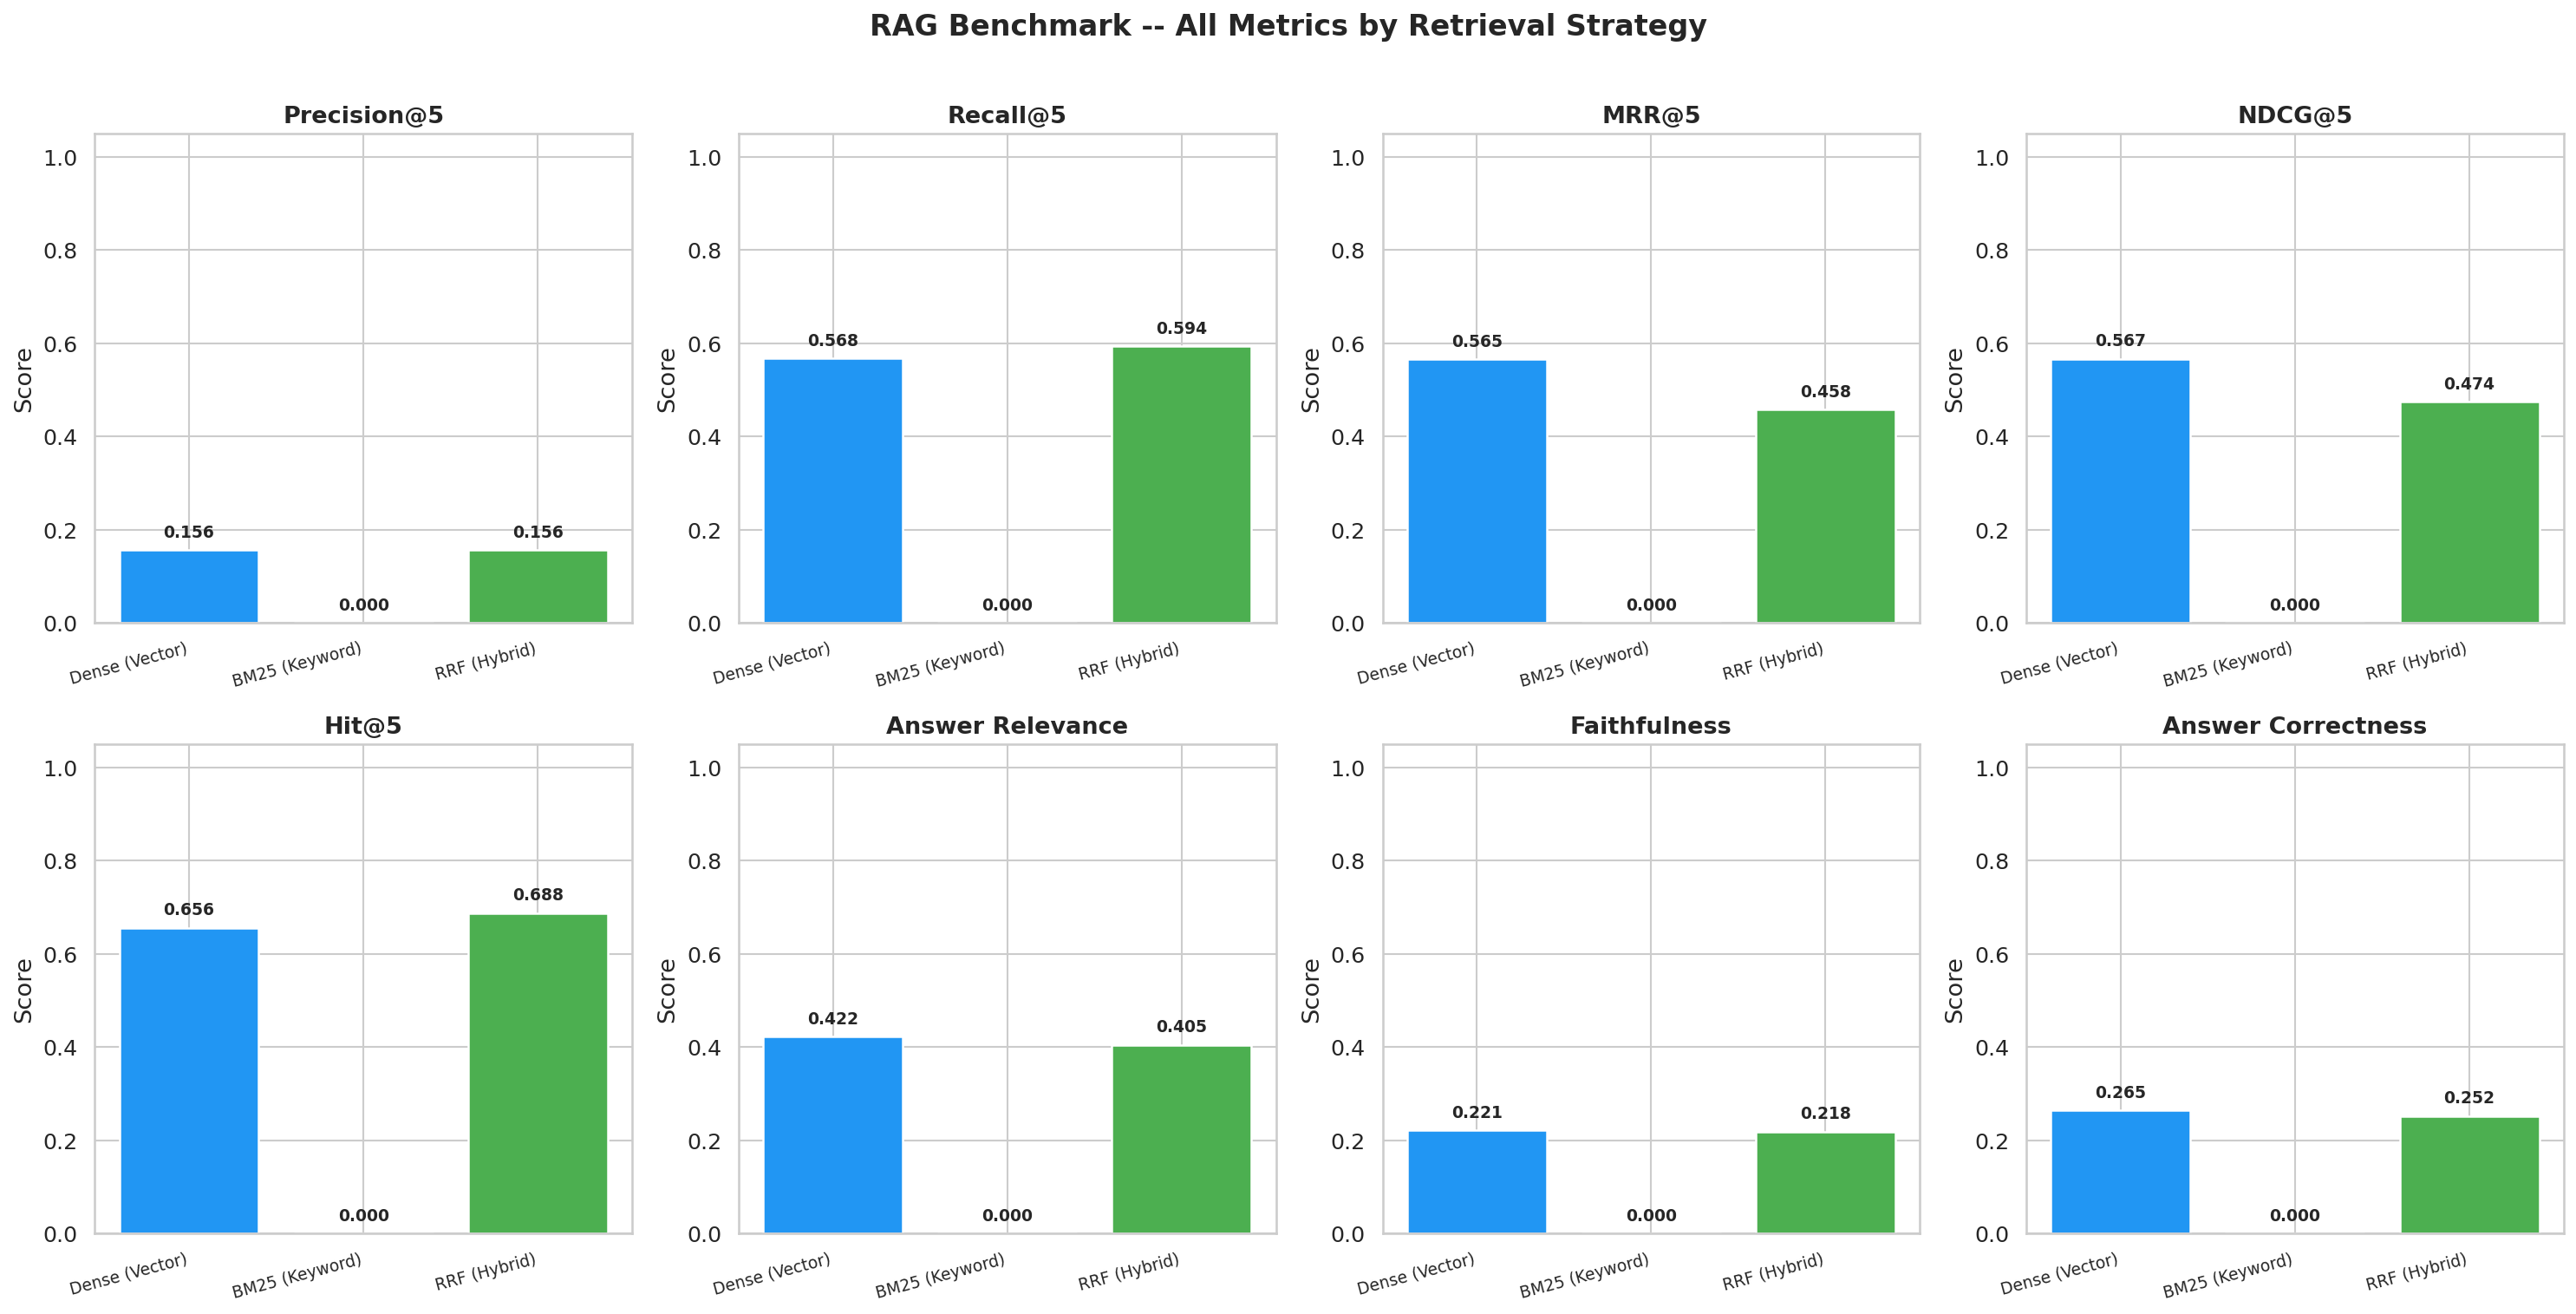
\includegraphics[width=\textwidth]{images/benchmark/fig1_all_metrics_bar.png}
\caption{Comparaison des 8 metriques par strategie de recherche --- diagrammes en barres}
\label{fig:all-metrics-bar}
\end{figure}

\subsection{Distributions des Metriques}

La Figure~\ref{fig:metric-distributions} presente les distributions des scores sous forme de boites a moustaches, revelant la variance par question :

\begin{figure}[h]
\centering
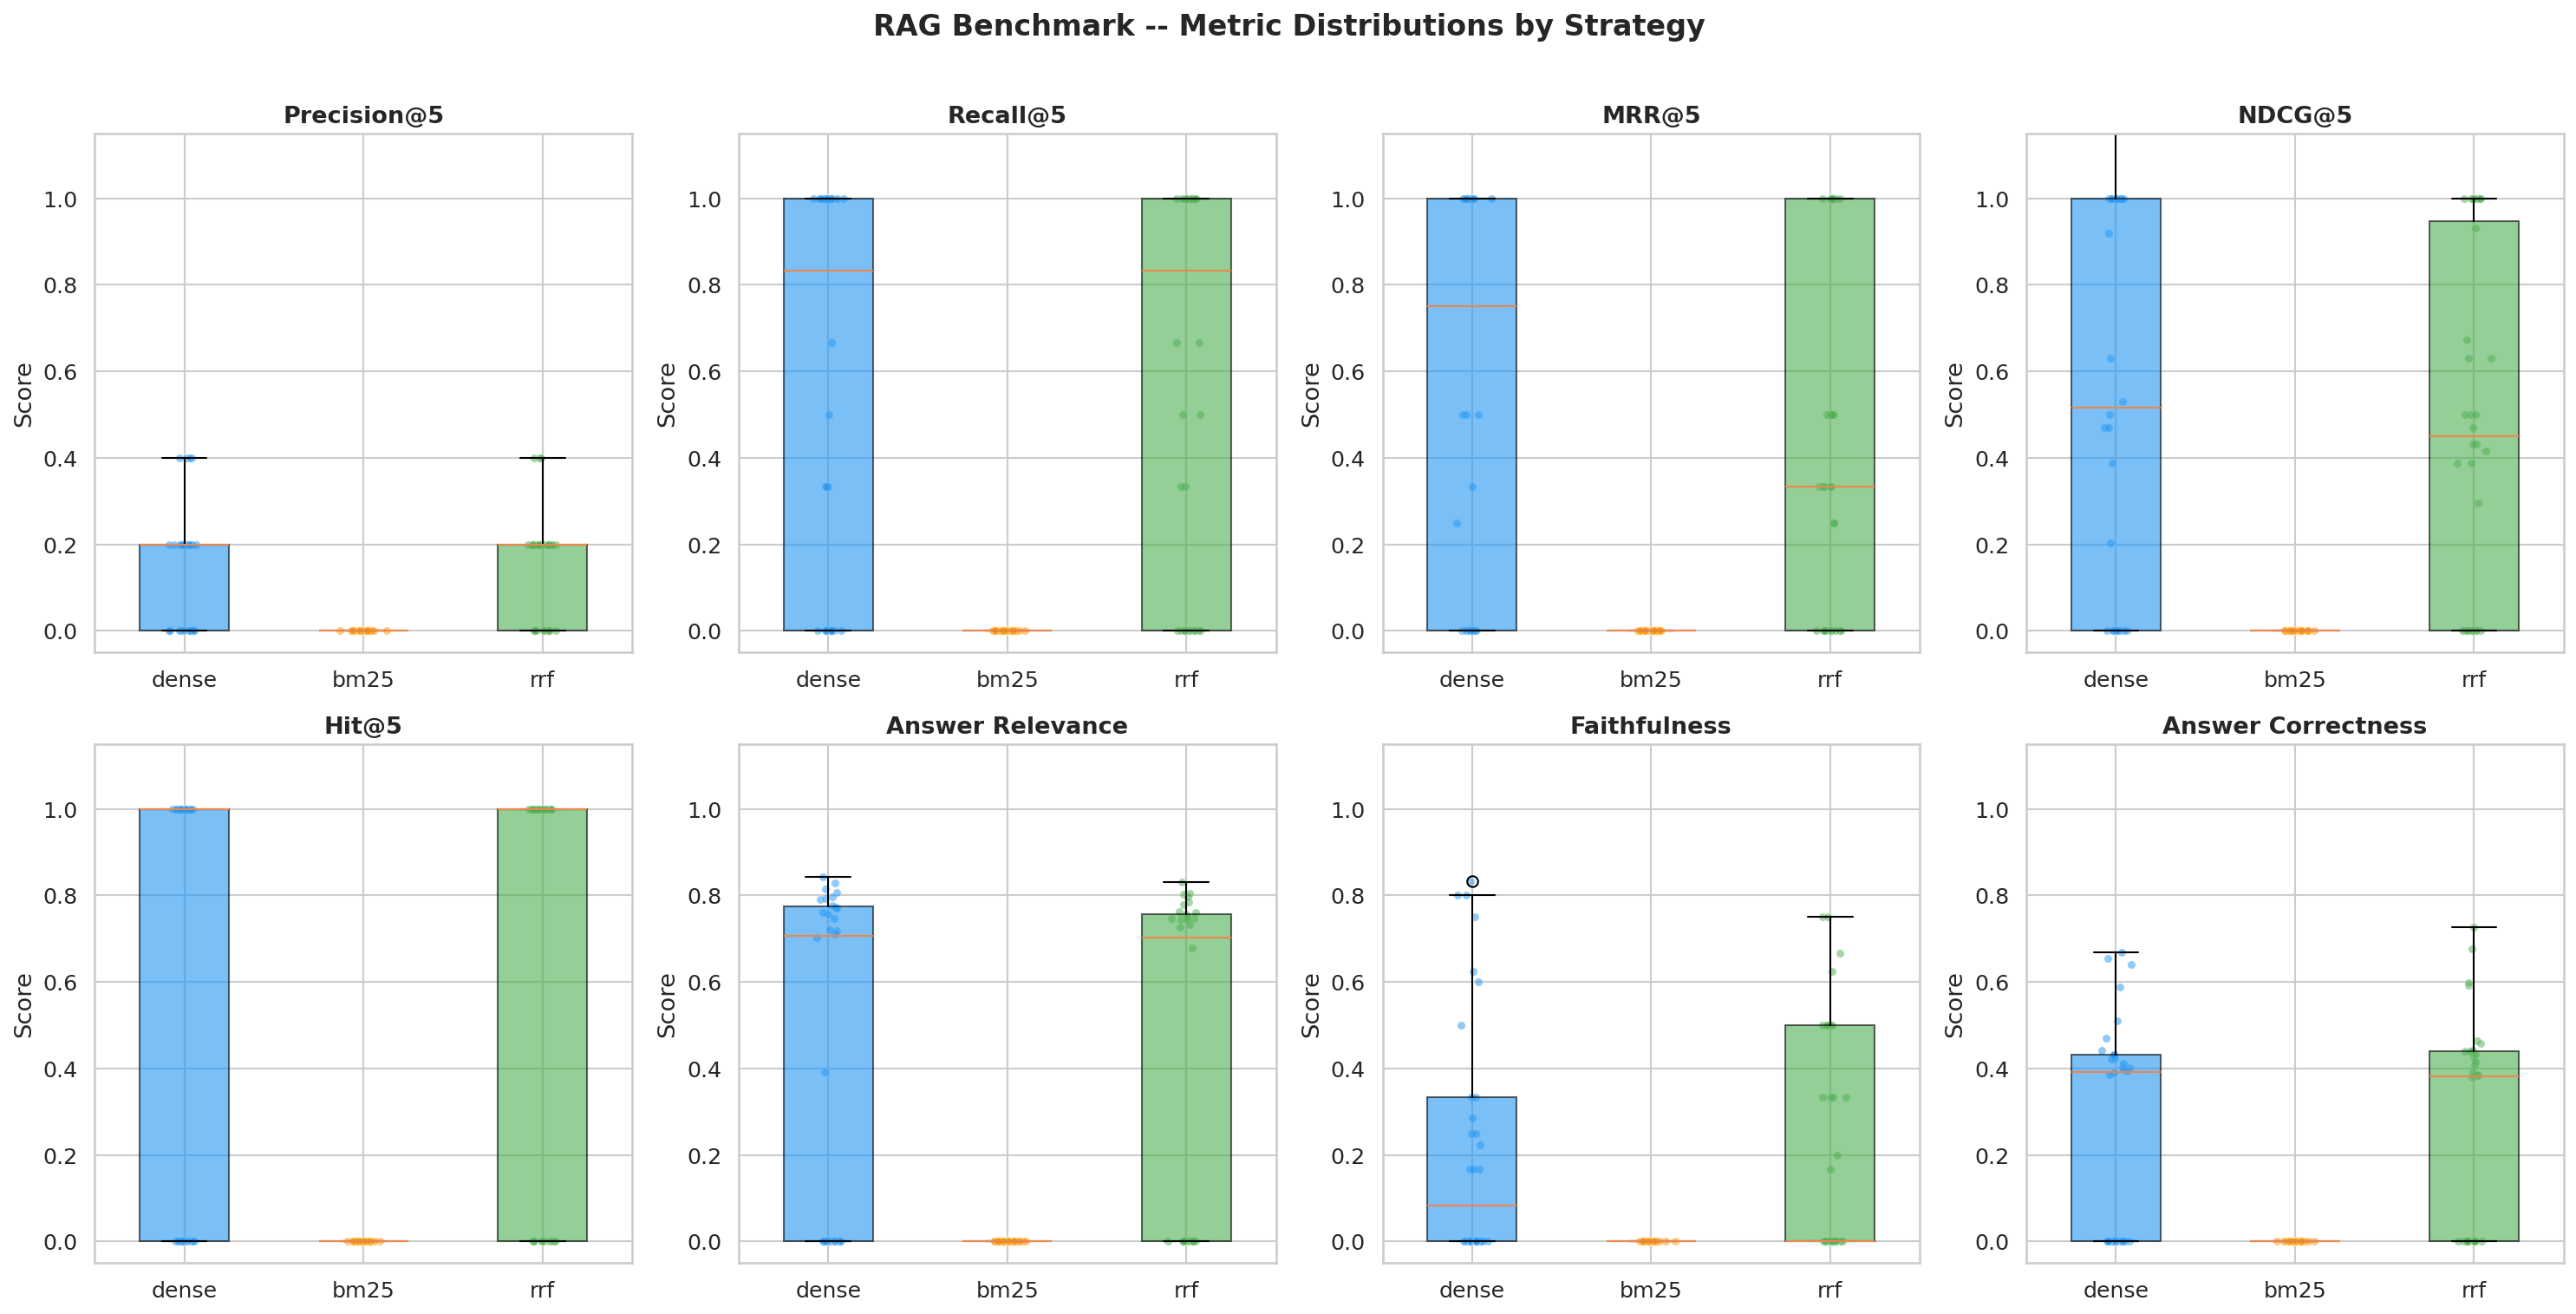
\includegraphics[width=\textwidth]{images/benchmark/fig2_metric_distributions.png}
\caption{Distributions des metriques par strategie --- boites a moustaches avec points individuels}
\label{fig:metric-distributions}
\end{figure}

On observe que :
\begin{itemize}
    \item BM25 est systematiquement a zero (aucune variance), confirmant l'echec complet de PostgreSQL FTS pour l'arabe.
    \item Dense et RRF presentent des distributions similaires, avec une legere superiority de RRF en Recall@5 et Hit@5, et de Dense en MRR@5 et NDCG@5.
    \item La variance est importante pour Faithfulness et Answer Correctness, indiquant une forte dependance a la question posee.
\end{itemize}

\subsection{Analyse Comparative Dense vs RRF}

La Figure~\ref{fig:radar-comparison} synthetise la comparaison Dense vs RRF sous forme de radar :

\begin{figure}[h]
\centering
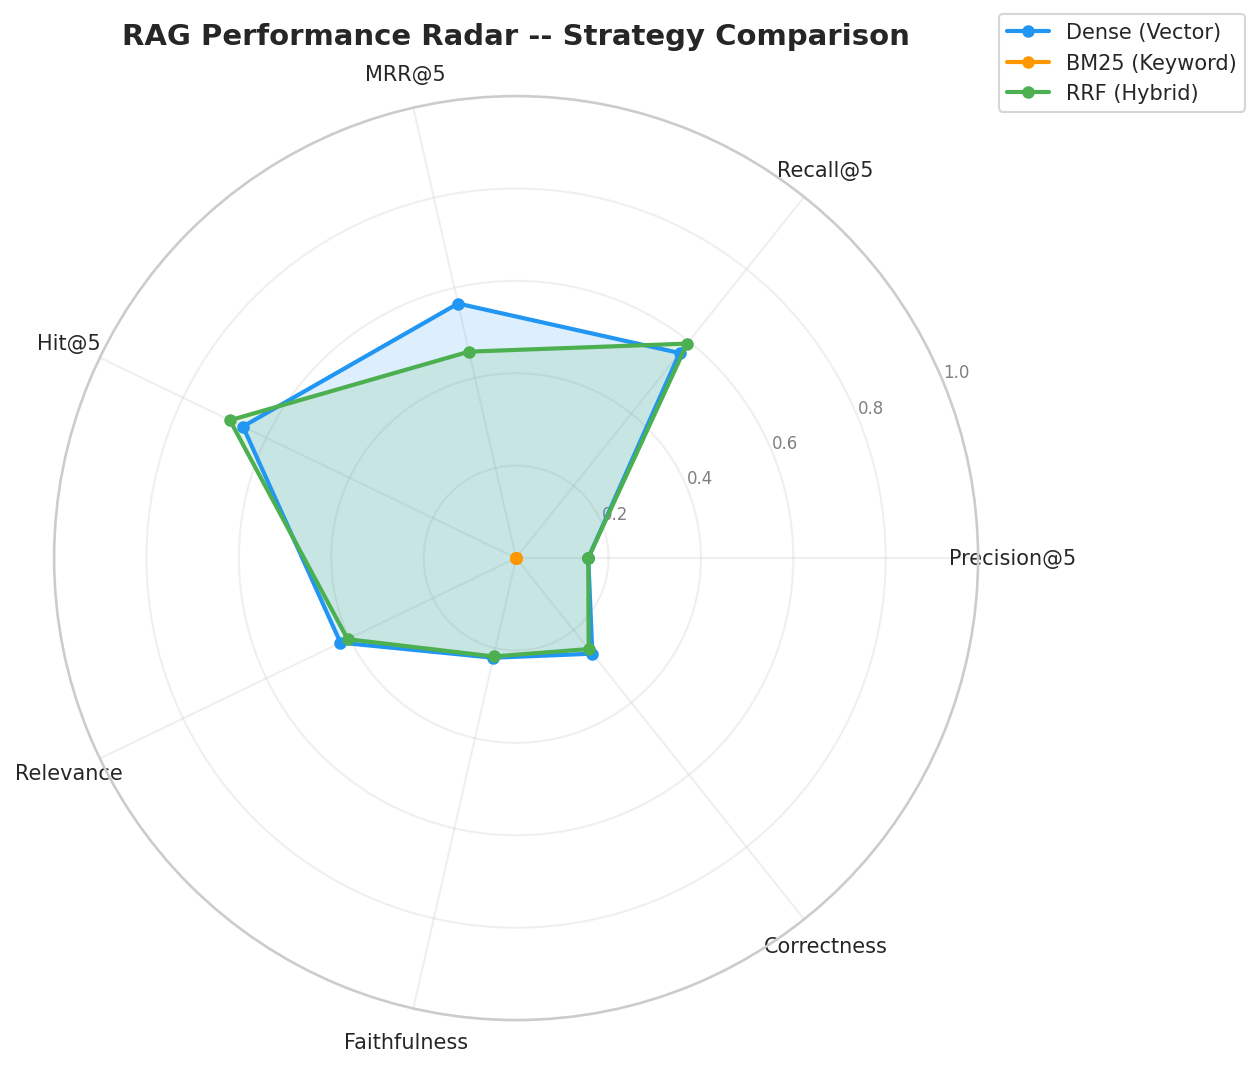
\includegraphics[width=0.6\textwidth]{images/benchmark/fig3_radar_comparison.png}
\caption{Comparaison radar des strategies --- Dense (bleu) vs RRF (vert) vs BM25 (orange, au centre)}
\label{fig:radar-comparison}
\end{figure}

Le radar confirme que Dense et RRF sont quasi-equivalents (le canal BM25 de RRF ne contribuait pas au moment du benchmark). Le Tableau~\ref{tab:dense-vs-rrf} quantifie les differences :

\begin{table}[h]
\centering
\renewcommand{\arraystretch}{1.3}
\begin{tabular}{|l|r|r|r|}
\hline
\rowcolor{LightBlue}
\textbf{\color{PrimaryBlue}Metrique} & \textbf{\color{PrimaryBlue}Dense} & \textbf{\color{PrimaryBlue}RRF} & \textbf{\color{PrimaryBlue}$\Delta$} \\
\hline
Hit@5 & 0.656 & 0.688 & +4.9\% (RRF) \\
Recall@5 & 0.568 & 0.594 & +4.6\% (RRF) \\
MRR@5 & 0.565 & 0.458 & $-$18.9\% (Dense) \\
NDCG@5 & 0.567 & 0.474 & $-$16.4\% (Dense) \\
Answer Relevance & 0.422 & 0.405 & $-$4.0\% (Dense) \\
Faithfulness & 0.221 & 0.219 & $-$0.9\% \\
Answer Correctness & 0.265 & 0.252 & $-$4.9\% \\
\hline
\end{tabular}
\caption{Comparaison detaillee Dense vs RRF}
\label{tab:dense-vs-rrf}
\end{table}

\textbf{Recommandation actuelle :} Utiliser la strategie Dense en production jusqu'a re-benchmarking avec le correctif BM25.

\subsection{Performance par Domaine Juridique (RRF)}

La Figure~\ref{fig:domain-heatmap} presente la performance de RRF par domaine juridique sous forme de carte de chaleur :

\begin{figure}[h]
\centering
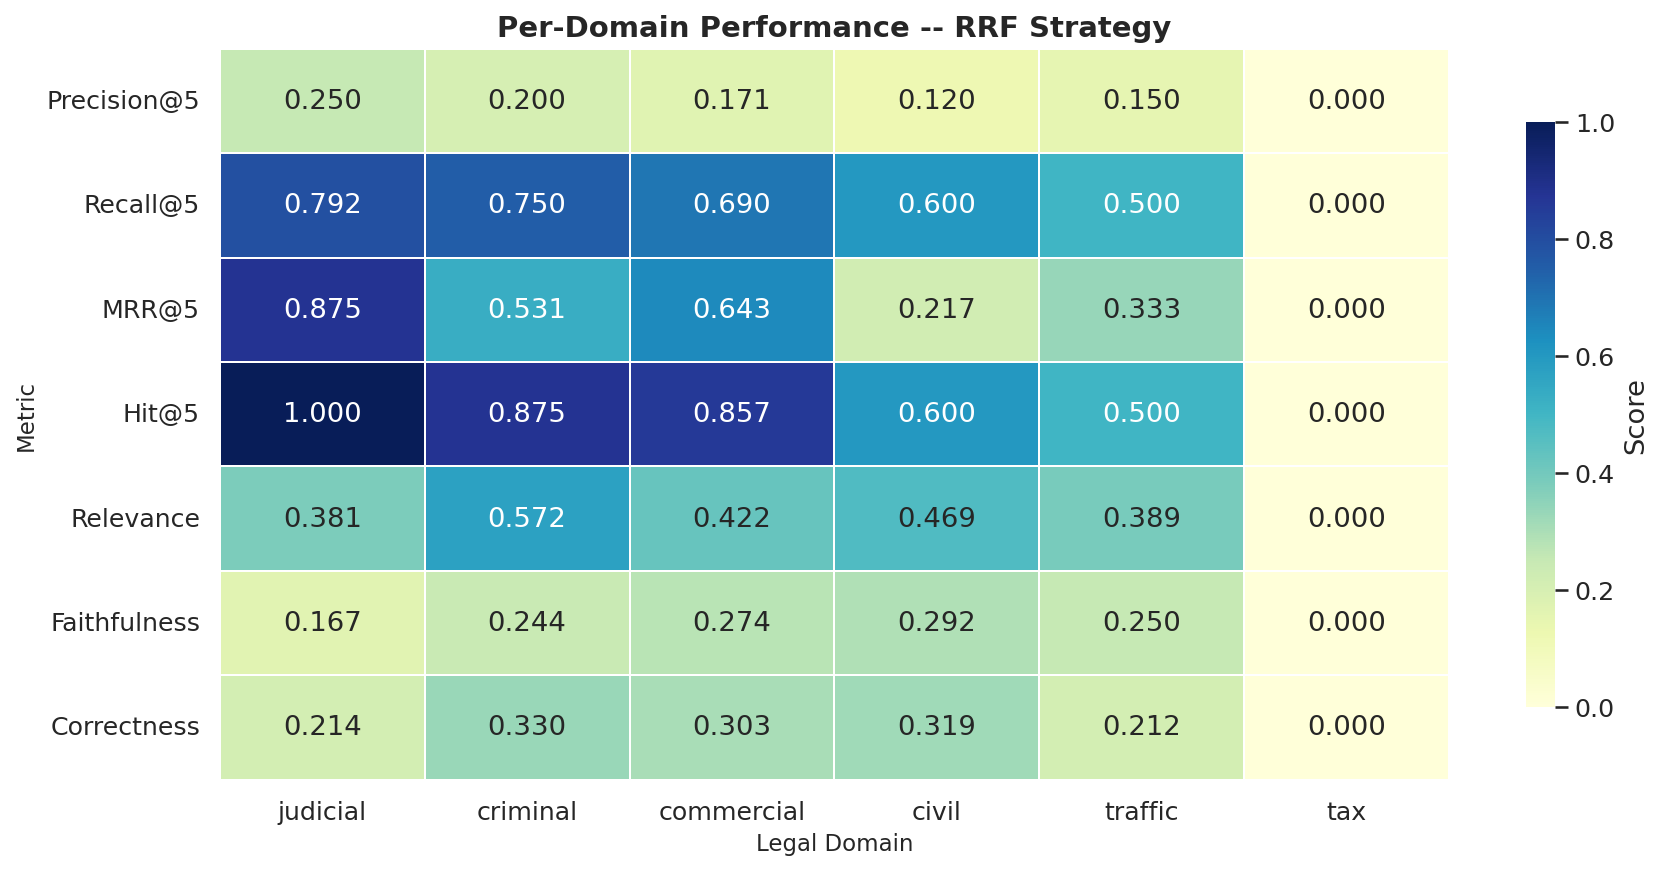
\includegraphics[width=\textwidth]{images/benchmark/fig4_domain_heatmap.png}
\caption{Performance par domaine juridique --- strategie RRF (carte de chaleur)}
\label{fig:domain-heatmap}
\end{figure}

Le Tableau~\ref{tab:rag-per-domain} extrait les valeurs numeriques :

\begin{table}[h]
\centering
\renewcommand{\arraystretch}{1.3}
\begin{tabular}{|l|r|r|r|r|r|}
\hline
\rowcolor{LightBlue}
\textbf{\color{PrimaryBlue}Domaine} & \textbf{\color{PrimaryBlue}Hit@5} & \textbf{\color{PrimaryBlue}Recall@5} & \textbf{\color{PrimaryBlue}Relevance} & \textbf{\color{PrimaryBlue}Faithfulness} & \textbf{\color{PrimaryBlue}Correctness} \\
\hline
Commercial & 0.714 & 0.690 & 0.544 & 0.512 & 0.452 \\
Criminal & 0.778 & 0.583 & 0.473 & 0.242 & 0.385 \\
Judicial & 0.500 & 0.792 & 0.253 & 0.167 & 0.214 \\
Civil & 0.400 & 0.600 & 0.481 & 0.307 & 0.346 \\
Traffic & 0.500 & 0.500 & 0.389 & 0.250 & 0.212 \\
Tax & 0.000 & 0.000 & 0.000 & 0.000 & 0.000 \\
\hline
\end{tabular}
\caption{Performance par domaine juridique --- RRF}
\label{tab:rag-per-domain}
\end{table}

\textbf{Analyse par domaine :}
\begin{itemize}
    \item \textbf{Commercial} (meilleur) : Hit@5 = 71.4\%, Faithfulness = 51.2\%. Le corpus ($\sim$359 articles) est bien structure et le vocabulaire specialise est bien capture par l'embedding.
    \item \textbf{Criminal} : Hit@5 = 77.8\% (meilleur taux de hit). Le corpus penal est le plus volumineux (822 articles).
    \item \textbf{Judicial} : Recall@5 = 79.2\% (meilleur rappel). Le petit corpus (32 articles) garantit un hit quasi-systematique, mais la qualite des reponses est faible (Relevance = 0.253).
    \item \textbf{Tax} (echec total) : Tous les scores sont a zero. Cause identifiee : \textbf{inadequation de domaine}. Les articles fiscaux sont stockes avec \texttt{domain = `civil'} dans la base, mais le benchmark les interroge avec \texttt{domain = `tax'}.
\end{itemize}

\subsection{Performance par Niveau de Difficulte (RRF)}

La Figure~\ref{fig:difficulty-breakdown} analyse les performances selon le niveau de difficulte des questions :

\begin{figure}[h]
\centering
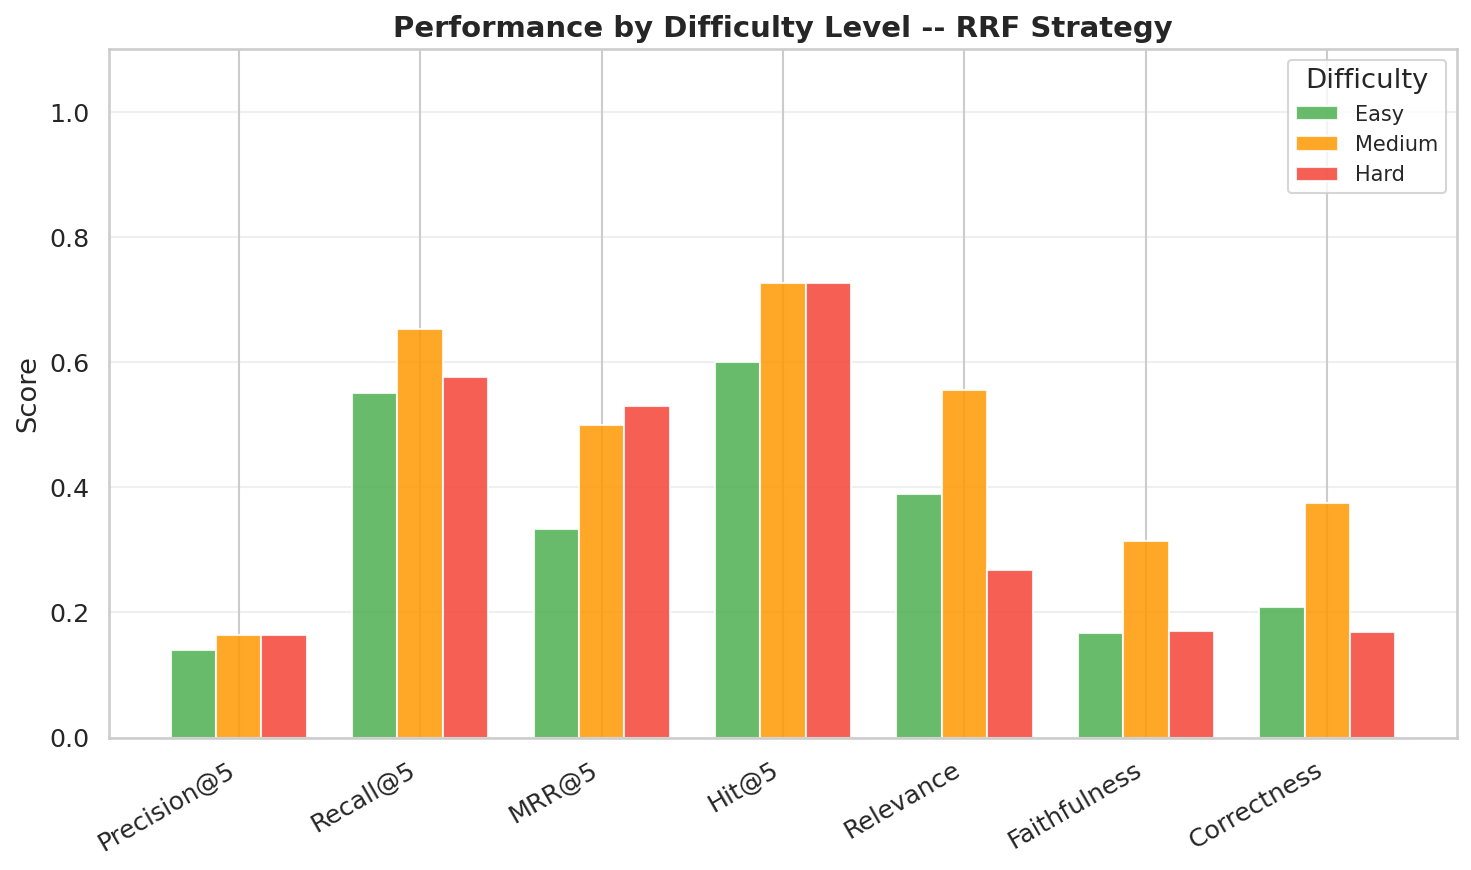
\includegraphics[width=0.9\textwidth]{images/benchmark/fig5_difficulty_breakdown.png}
\caption{Performance par niveau de difficulte --- RRF}
\label{fig:difficulty-breakdown}
\end{figure}

\begin{table}[h]
\centering
\renewcommand{\arraystretch}{1.3}
\begin{tabular}{|l|r|r|r|r|r|}
\hline
\rowcolor{LightBlue}
\textbf{\color{PrimaryBlue}Difficulte} & \textbf{\color{PrimaryBlue}Hit@5} & \textbf{\color{PrimaryBlue}Recall@5} & \textbf{\color{PrimaryBlue}Relevance} & \textbf{\color{PrimaryBlue}Faithfulness} & \textbf{\color{PrimaryBlue}Correctness} \\
\hline
Easy (10 questions) & 0.700 & 0.633 & 0.442 & 0.245 & 0.265 \\
Medium (11 questions) & 0.636 & 0.576 & 0.424 & 0.222 & 0.269 \\
Hard (11 questions) & 0.727 & 0.576 & 0.486 & 0.242 & 0.306 \\
\hline
\end{tabular}
\caption{Performance par niveau de difficulte --- RRF}
\label{tab:rag-per-difficulty}
\end{table}

\textbf{Constat contre-intuitif :} Les questions difficiles (\textit{hard}) performent mieux que les questions moyennes (\textit{medium}) sur Hit@5 (+14\%), Answer Relevance (+15\%), et Answer Correctness (+14\%). Ce phenomene s'explique par la specificite du vocabulaire juridique : les questions difficiles utilisent des termes plus techniques et distinctifs, mieux captures par l'embedding semantique.

\subsection{Latence du Pipeline}

La Figure~\ref{fig:latency} decompose la latence du pipeline complet par strategie :

\begin{figure}[h]
\centering
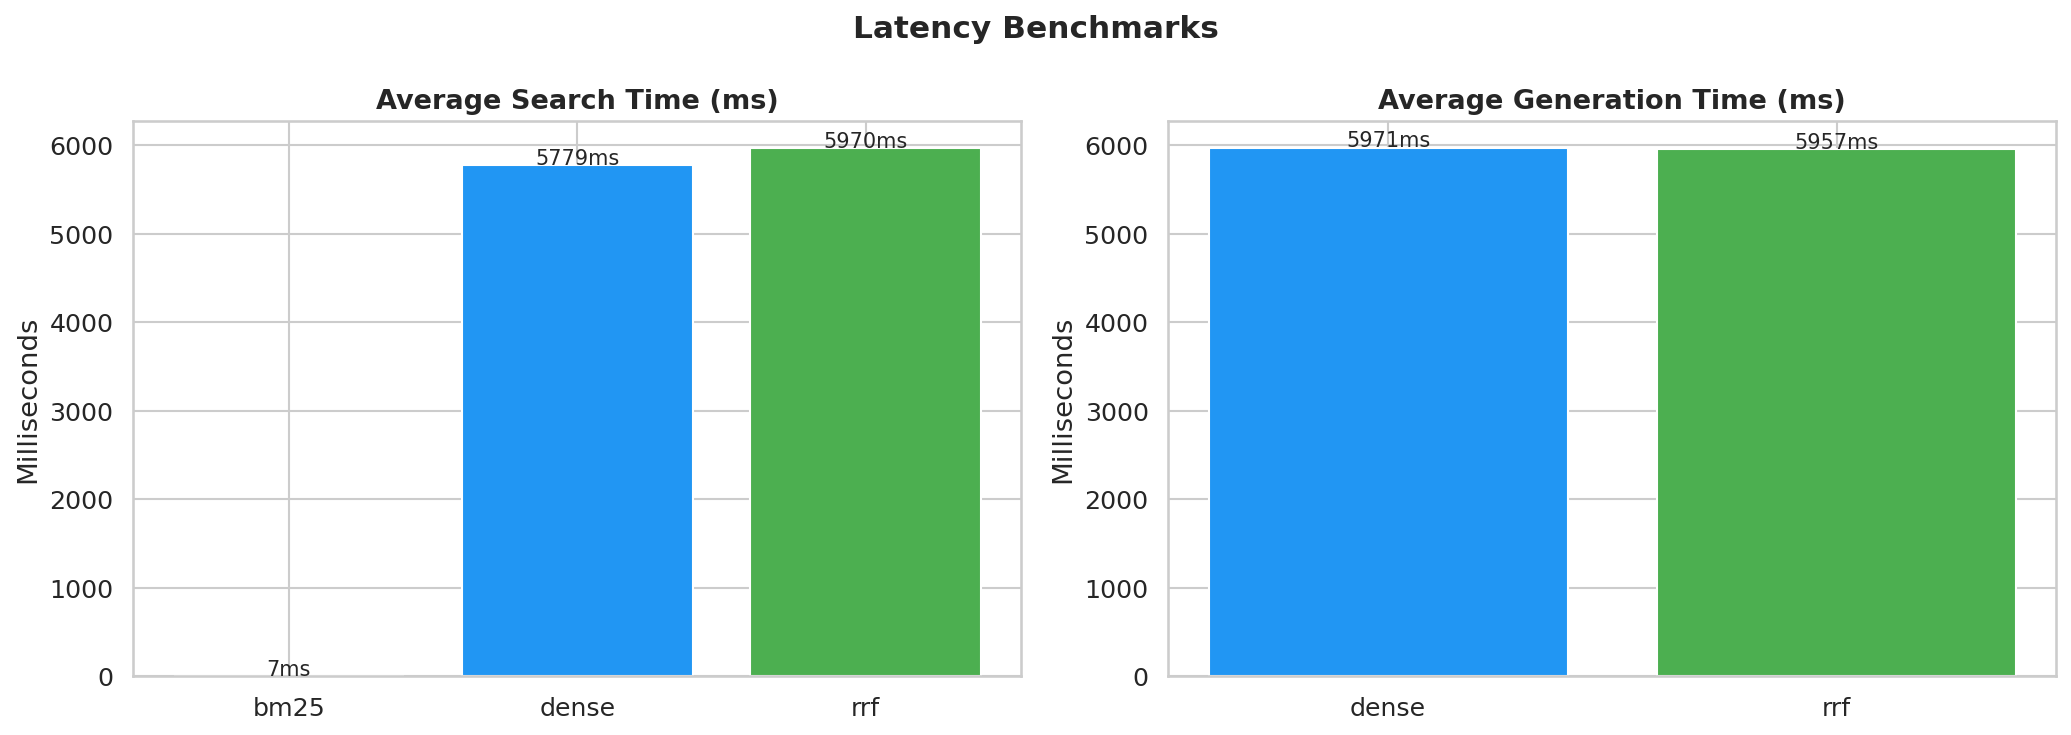
\includegraphics[width=0.9\textwidth]{images/benchmark/fig6_latency_comparison.png}
\caption{Latence du pipeline --- temps de recherche et de generation par strategie}
\label{fig:latency}
\end{figure}

\begin{table}[h]
\centering
\renewcommand{\arraystretch}{1.3}
\begin{tabular}{|l|r|r|r|}
\hline
\rowcolor{LightBlue}
\textbf{\color{PrimaryBlue}Composant} & \textbf{\color{PrimaryBlue}BM25} & \textbf{\color{PrimaryBlue}Dense} & \textbf{\color{PrimaryBlue}RRF} \\
\hline
Recherche (ms) & 7 & 5\,779 & 5\,970 \\
Generation (ms) & 0 & 5\,971 & 5\,957 \\
\textbf{Total (ms)} & \textbf{7} & \textbf{11\,750} & \textbf{11\,927} \\
\hline
\end{tabular}
\caption{Latence moyenne du pipeline par strategie}
\label{tab:rag-latency}
\end{table}

La latence de BM25 est negligeable (7 ms, aucune recherche effective). Pour Dense et RRF, la latence totale est d'environ 12 secondes, repartie equitablement entre la recherche (49\%) et la generation (51\%). Le goulot d'etranglement est le service d'embedding distant via Cloudflare Tunnel ($\sim$5.5 s). Un deploiement local reduirait cette latence a $\sim$100 ms, divisant le temps total par 2.

\subsection{Analyse de la Fidelite (Faithfulness)}

La metrique de fidelite affiche des scores bas (20-22\%) qui \textbf{ne doivent pas etre interpretes comme un taux d'hallucination}. L'analyse qualitative des reponses revele que le LLM produit un enrichissement contextuel legitime non detecte par le chevauchement lexical :

\begin{itemize}
    \item \textbf{Synthese multi-articles} : Le LLM combine des informations de plusieurs articles pour formuler une conclusion juridique. Cette synthese est semantiquement aneree mais ne correspond a aucune sous-chaine exacte.
    \item \textbf{Citations structurees} : Les references du type \textarabic{«~حسب المادة 513 من القانون الجنائي~»} sont des formulations originales du LLM absentes des documents sources.
    \item \textbf{Reformulation juridique} : Le LLM reformule le langage legislatif en langage explicatif plus accessible.
\end{itemize}

\textbf{Recommandation :} Remplacer la metrique de chevauchement lexical par une evaluation LLM-as-judge capable d'evaluer la fidelite semantique.

\section{Synthese des Resultats}

Le Tableau~\ref{tab:results-synthesis} synthetise les resultats des trois campagnes de benchmark :

\begin{table}[h]
\centering
\renewcommand{\arraystretch}{1.3}
\begin{tabular}{|l|p{5cm}|r|}
\hline
\rowcolor{LightBlue}
\textbf{\color{PrimaryBlue}Benchmark} & \textbf{\color{PrimaryBlue}Resultat principal} & \textbf{\color{PrimaryBlue}Valeur} \\
\hline
Embedding (5 modeles) & E5-large recommande & P@1 = 72\%, MRR = 81\% \\
Strategies (4 strategies) & RRF recommande (sans parametre) & Recall@K = 71\%, MRR = 0.57 \\
RAG complet (32 questions) & Dense operationnel, RRF equivalent & Hit@5 = 65-69\% \\
\hline
\end{tabular}
\caption{Synthese des resultats des trois campagnes de benchmark}
\label{tab:results-synthesis}
\end{table}

Les principaux enseignements :

\begin{enumerate}
    \item \textbf{E5-large est le modele d'embedding optimal} pour l'arabe juridique marocain, avec une marge significative sur les modeles 768d et une interchangeabilite avec BGE-M3.

    \item \textbf{La recherche dense est operationnelle et efficace}, avec 65-69\% de taux de hit sur le corpus complet et 89\% de precision de domaine.

    \item \textbf{Le BM25 necessite une re-evaluation} apres l'application du correctif de tokenisation arabe (Section~\ref{sec:conception-bm25}). Les resultats actuels (zero) refletent un bug d'implementation PostgreSQL, pas une incapacite intrinseque.

    \item \textbf{Le domaine fiscal est inaccessible} en raison d'une inadequation de taxonomie entre le benchmark (\texttt{domain = `tax'}) et la base de donnees (\texttt{domain = `civil'}).

    \item \textbf{La fidelite est sous-estimee} par la metrique de chevauchement lexical. L'enrichissement contextuel (synthese, citations, reformulation) est un comportement souhaite.

    \item \textbf{La latence est dominee par le tunnel Cloudflare} ($\sim$5.5 s sur $\sim$12 s). Un deploiement local de l'embedding diviserait le temps de reponse par deux.

    \item \textbf{Les questions difficiles performent mieux} que les questions moyennes, suggerant que la specificite du vocabulaire juridique est un avantage pour la recherche semantique.
\end{enumerate}


\section{Capture d'ecrans de l'interface}

\subsection{Page d'Accueil}

La page d'accueil constitue le point d'entrée principal de la plateforme. Elle permet aux utilisateurs de poser des questions juridiques en arabe à travers une interface simple et intuitive. Des catégories juridiques prédéfinies et des exemples de requêtes facilitent l'exploration des différents domaines du droit marocain. La page propose également le téléversement de documents juridiques pour leur analyse automatisée par le système.

\begin{figure}[H]
\centering
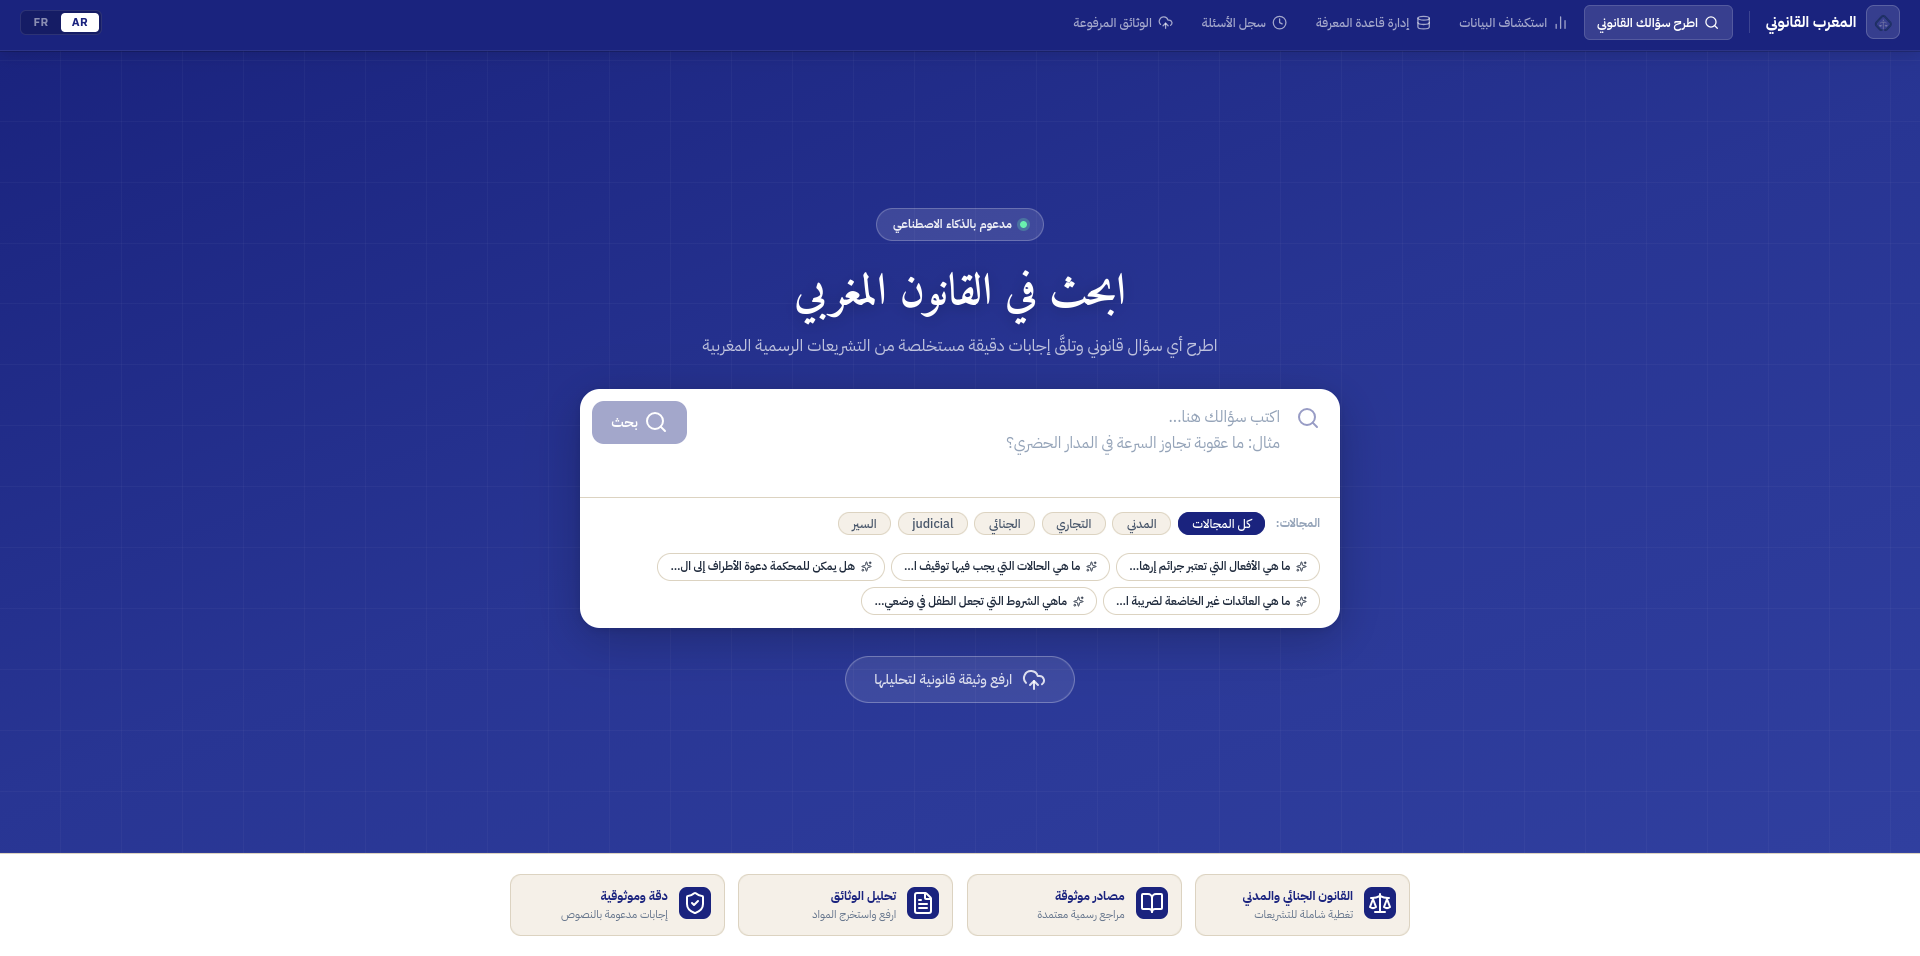
\includegraphics[width=\textwidth]{images/screenshots/home-page.png}
\caption{Homepage of the Moroccan Legal RAG platform.}
\label{fig:home-page}
\end{figure}


\subsection{Exploration de la Base de Connaissances}

Cette interface permet d'explorer directement la base de connaissances juridique indexée par le système. L'utilisateur peut soumettre une requête, sélectionner un domaine juridique et choisir une stratégie de recherche (Dense, BM25 ou Hybride RRF). Elle facilite l'analyse des résultats récupérés et l'évaluation des différentes méthodes de recherche implémentées dans la plateforme.


\begin{figure}[H]
\centering
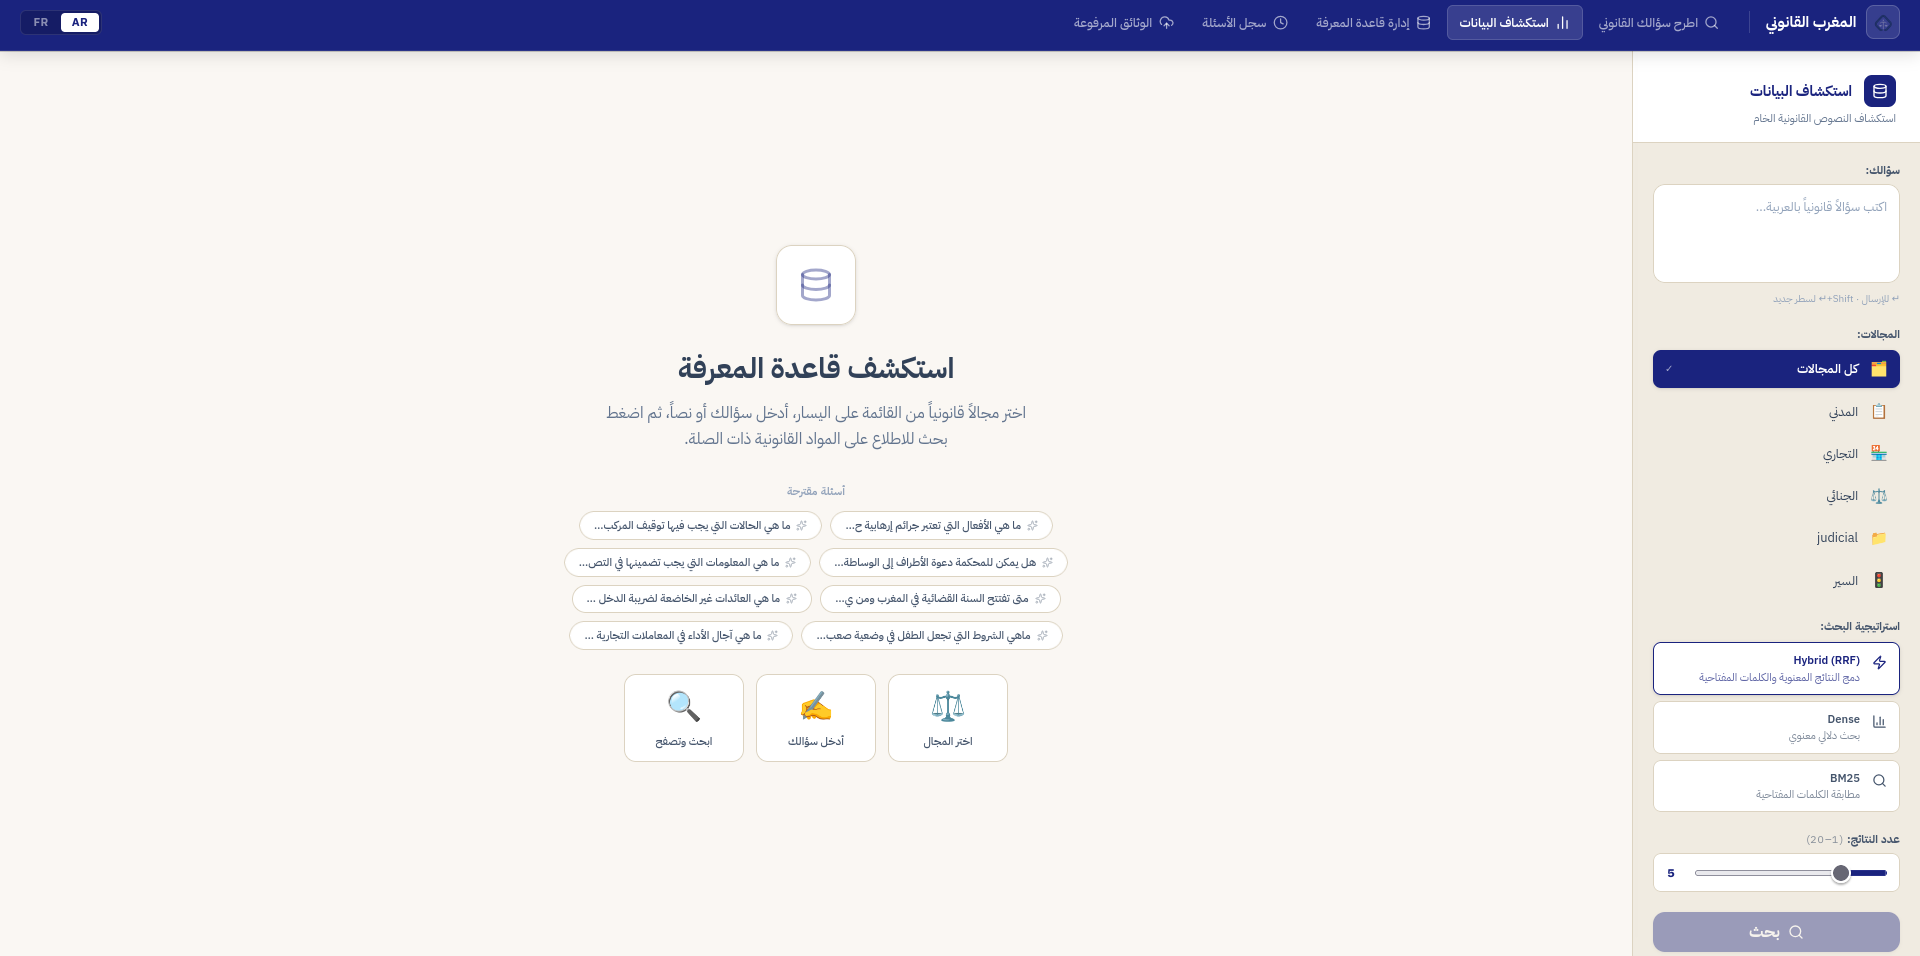
\includegraphics[width=\textwidth]{images/screenshots/knowledge-base-explorer-1.png}
\caption{Interface d'exploration de la base de connaissances juridique.}
\label{fig:knowledge-base-explorer-1}
\end{figure}


\begin{figure}[H]
\centering
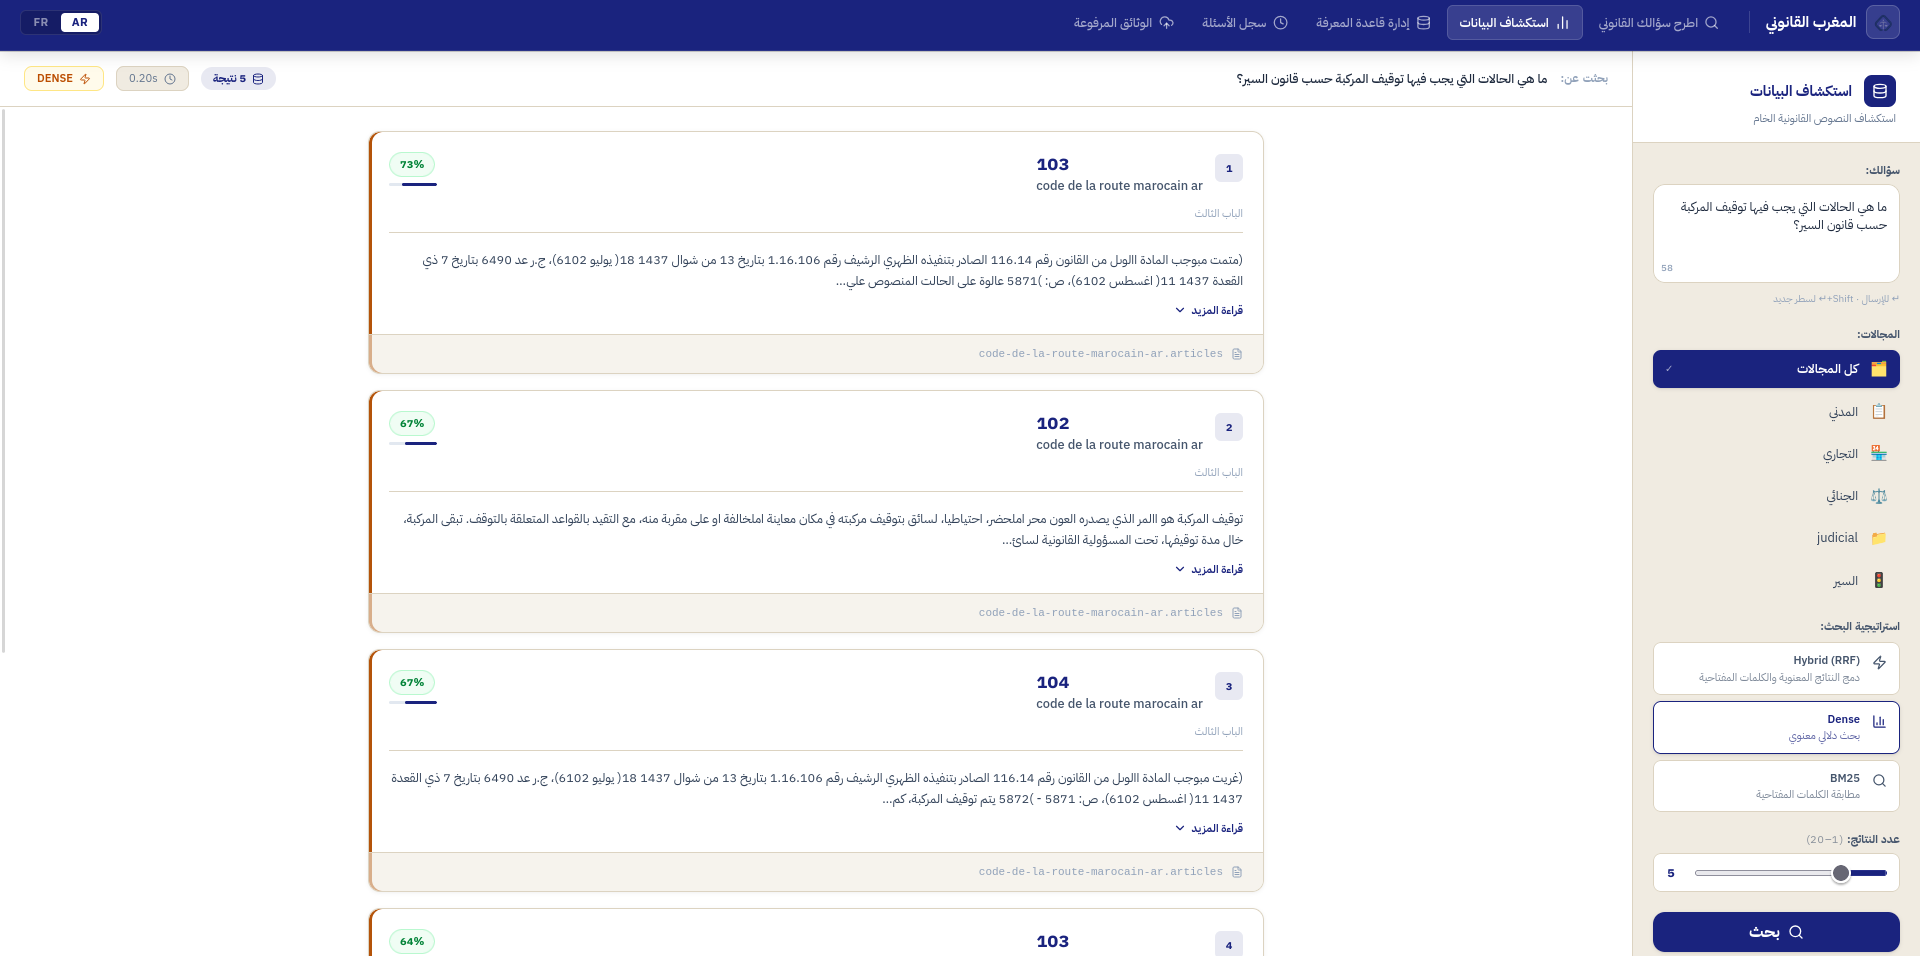
\includegraphics[width=\textwidth]{images/screenshots/knowledge-base-explorer-2.png}
\caption{Interface d'exploration de la base de connaissances juridique.}
\label{fig:knowledge-base-explorer-2}
\end{figure}


\subsection{Gestion de la Base de Connaissances}

Cette interface permet d'administrer les documents juridiques indexés dans la base de connaissances. Elle offre des fonctionnalités de téléversement, de consultation et de gestion des textes législatifs, tout en affichant des statistiques sur le nombre de lois, d'articles et de domaines juridiques disponibles. Les documents peuvent être activés ou désactivés afin de contrôler leur participation au processus de recherche et de génération des réponses.


\begin{figure}[H]
\centering
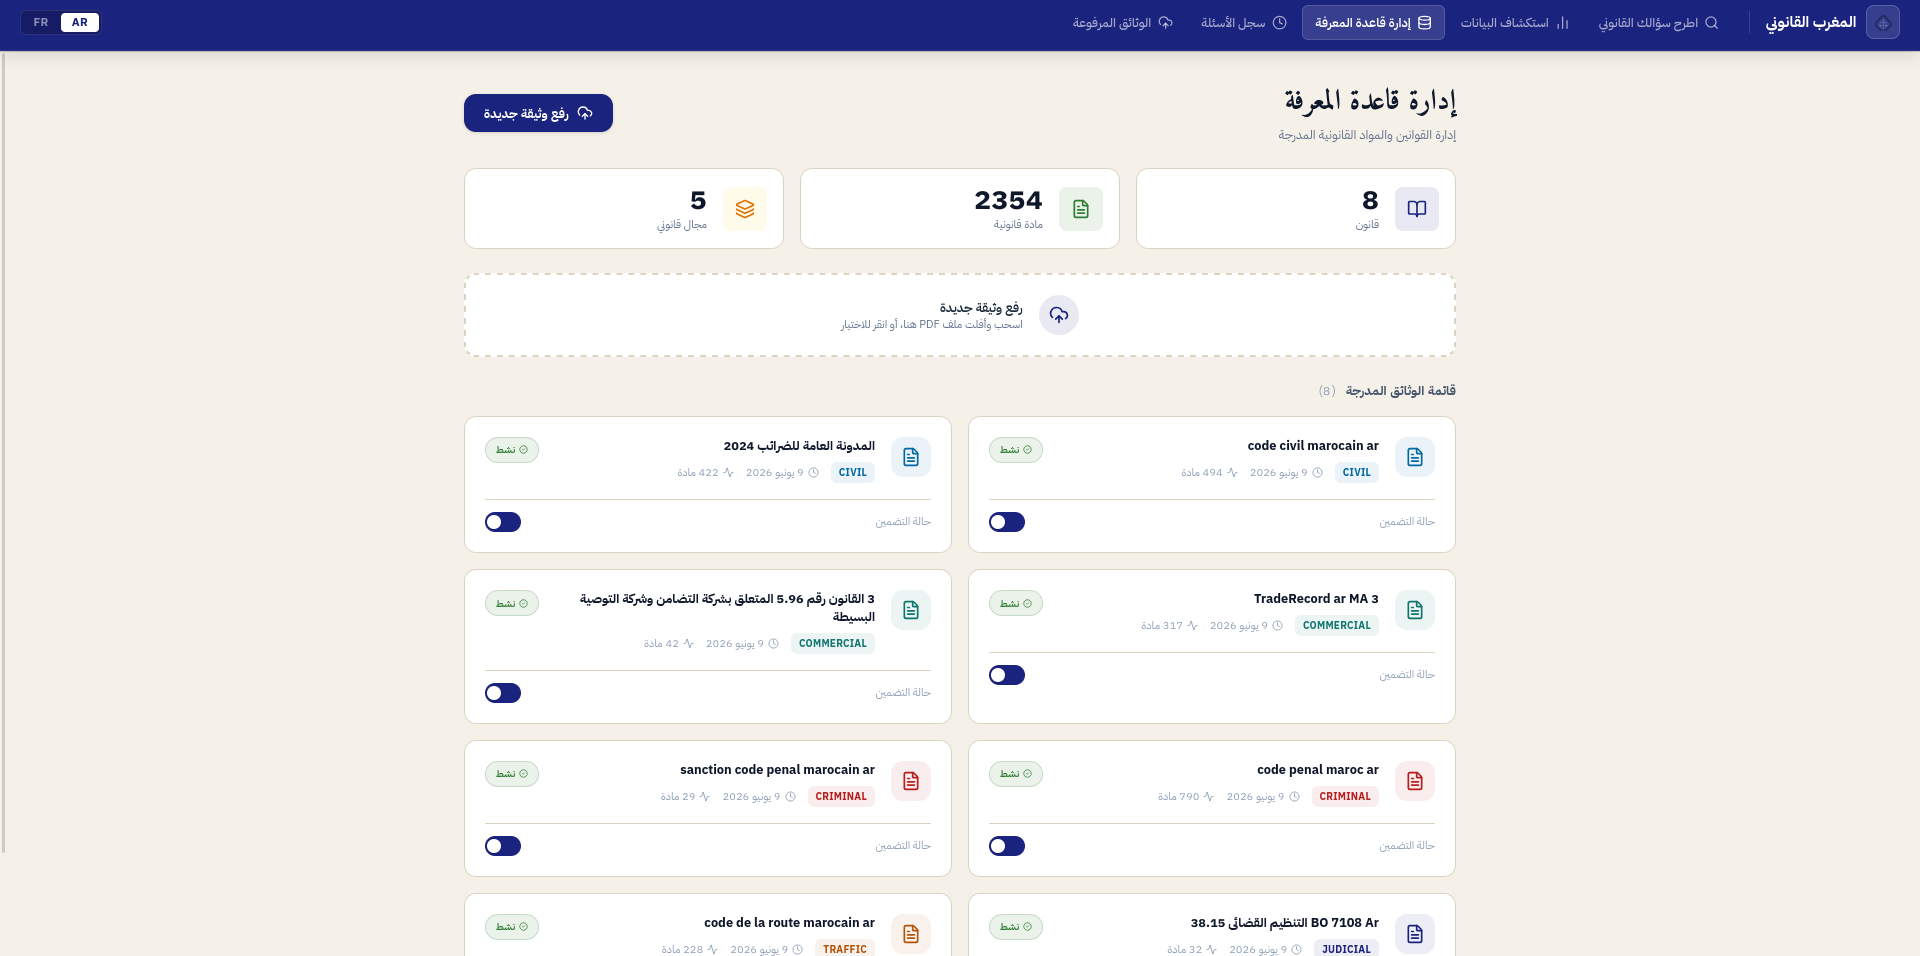
\includegraphics[width=\textwidth]{images/screenshots/knowledge-base-management.png}
\caption{Interface de gestion de la base de connaissances.}
\label{fig:knowledge-base-management}
\end{figure}


\subsection{Historique des Conversations}

Cette interface permet de consulter l'historique des questions posées à la plateforme. Les utilisateurs peuvent rechercher, parcourir et reprendre d'anciennes conversations afin de retrouver rapidement des réponses juridiques précédemment générées. Elle facilite le suivi des échanges et améliore la continuité de l'expérience utilisateur.

\begin{figure}[H]
\centering
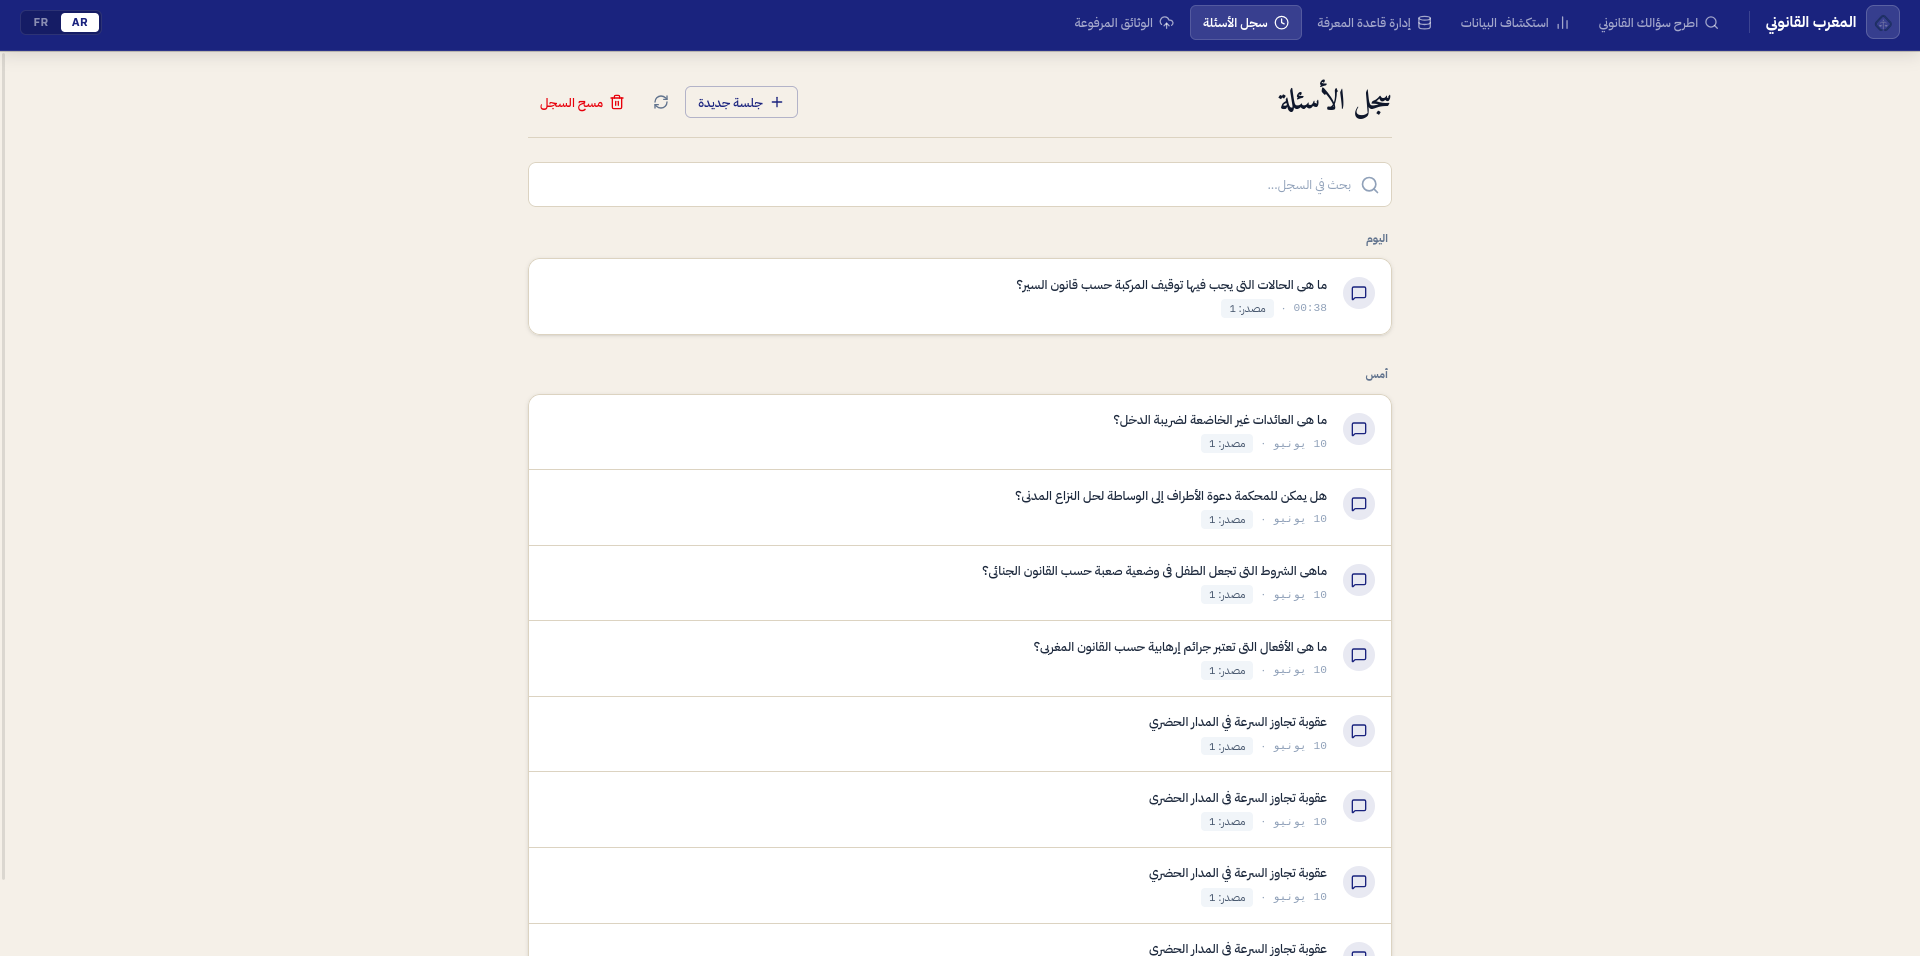
\includegraphics[width=\textwidth]{images/screenshots/conversation-history.png}
\caption{Interface d'historique des conversations.}
\label{fig:conversation-history}
\end{figure}


\subsection{Téléversement et Traitement des Documents Juridiques}

Cette interface permet aux utilisateurs de téléverser des documents juridiques au format PDF pour un traitement automatisé. Le système extrait le contenu du document, identifie les articles juridiques et les transforme en données structurées pouvant être intégrées à la base de connaissances. La page affiche également l'historique des documents traités ainsi que le nombre d'articles extraits pour chaque fichier.


\begin{figure}[H]
\centering
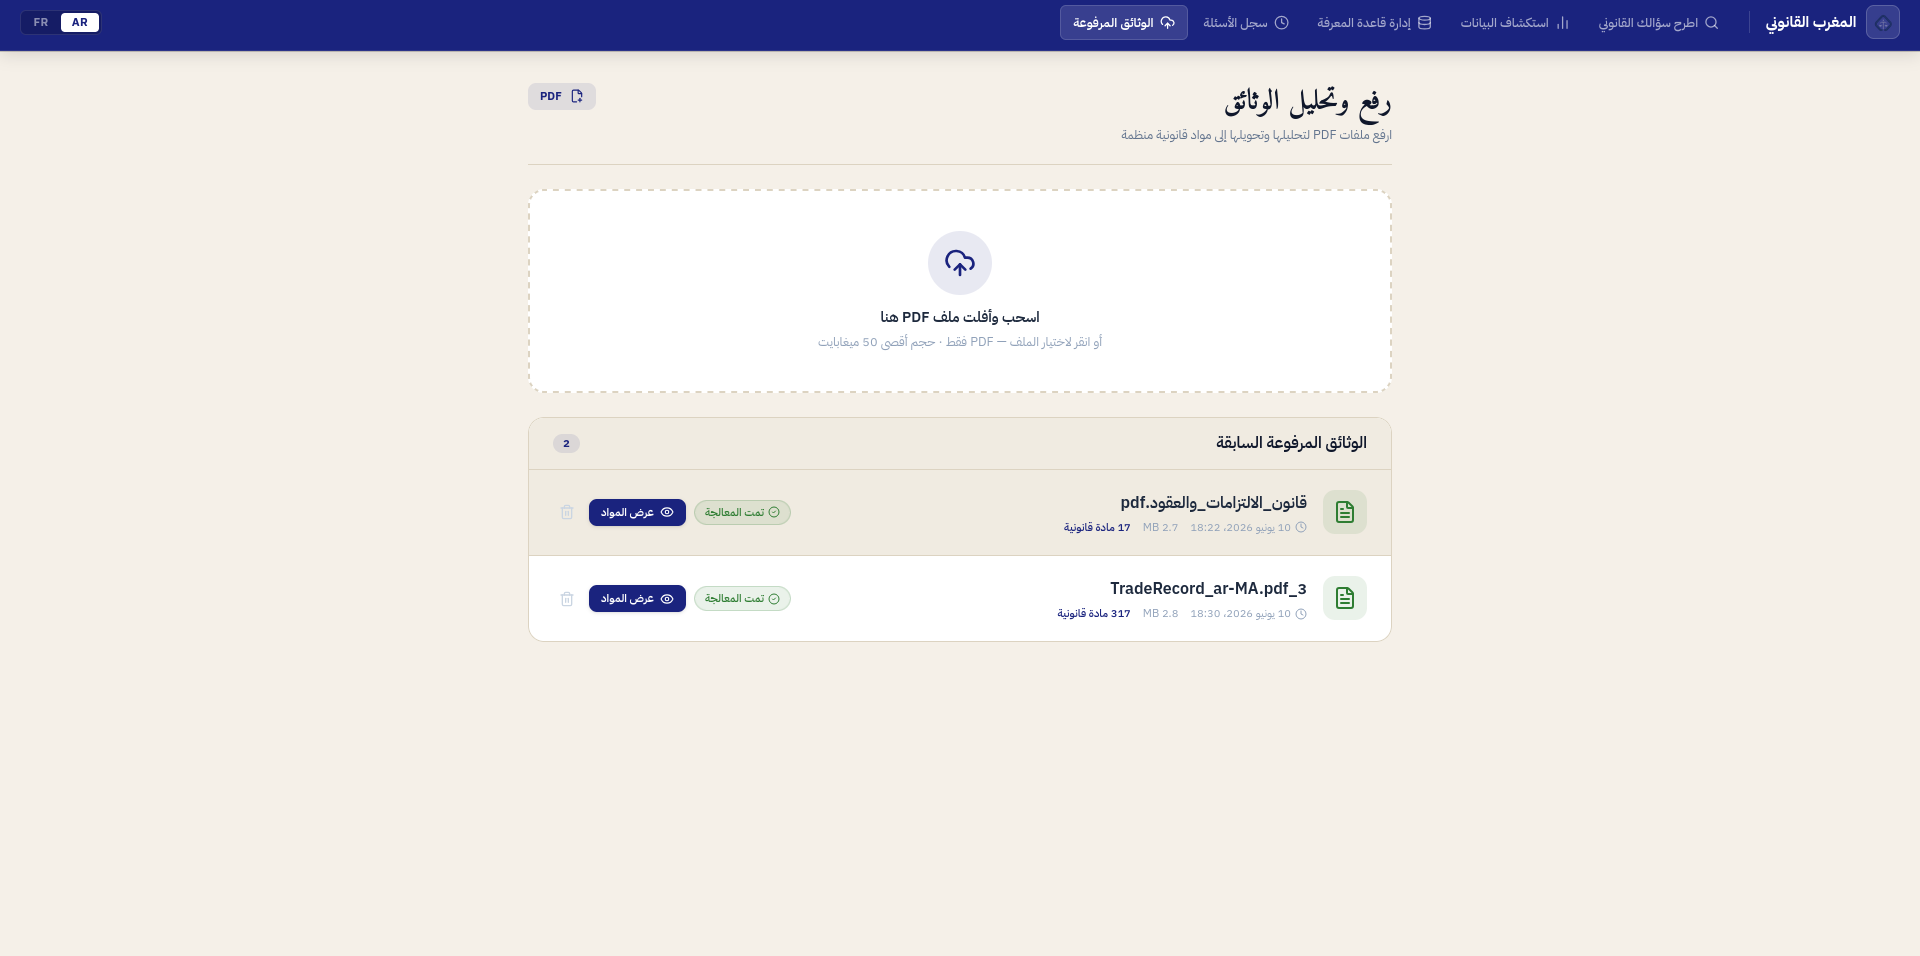
\includegraphics[width=\textwidth]{images/screenshots/document-upload-processing-1.png}
\caption{Interface de téléversement et de traitement des documents juridiques.}
\label{fig:document-upload-processing-1}
\end{figure}

\begin{figure}[H]
\centering
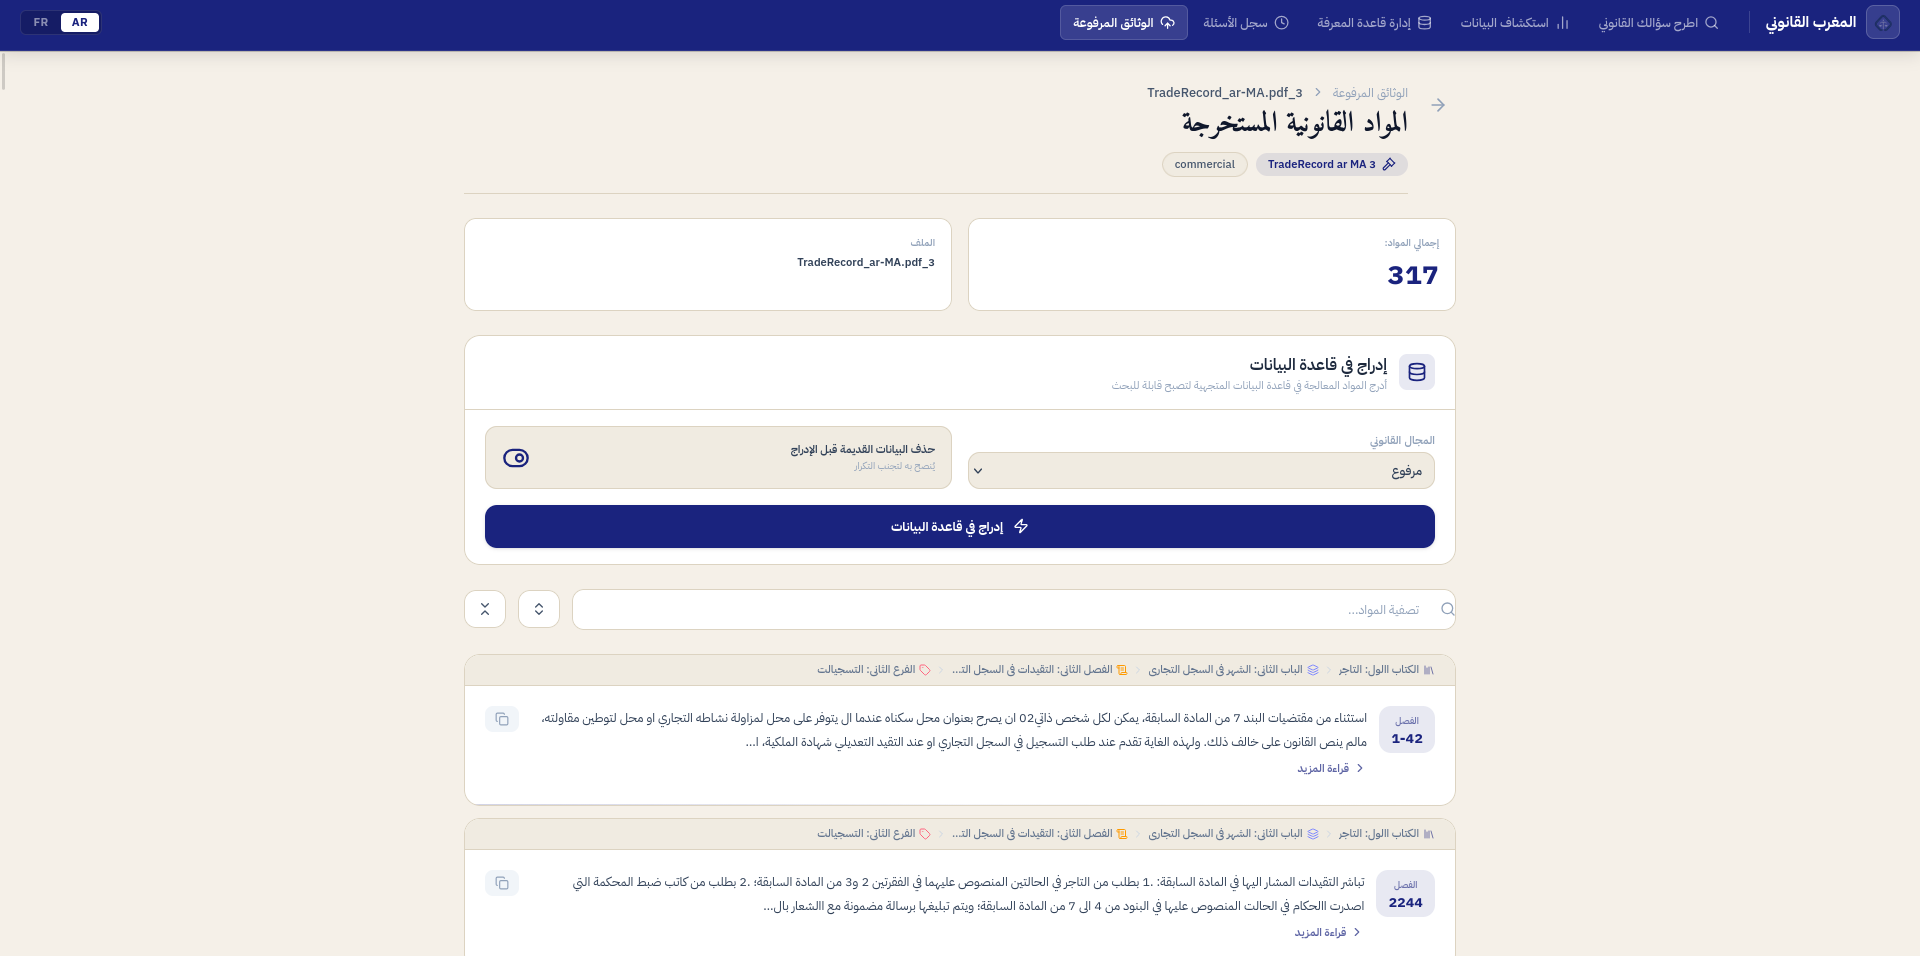
\includegraphics[width=\textwidth]{images/screenshots/document-upload-processing-2.png}
\caption{Interface de téléversement et de traitement des documents juridiques.}
\label{fig:document-upload-processing-2}
\end{figure}


\subsection{Interface Conversationnelle}

Cette interface constitue le cœur du système de question-réponse juridique. Elle affiche la réponse générée par le modèle ainsi que les sources légales utilisées pour sa génération. Les passages juridiques pertinents sont présentés avec leur score de pertinence, permettant à l'utilisateur de vérifier l'origine des informations et d'assurer la transparence du processus de génération.

\begin{figure}[H]
\centering
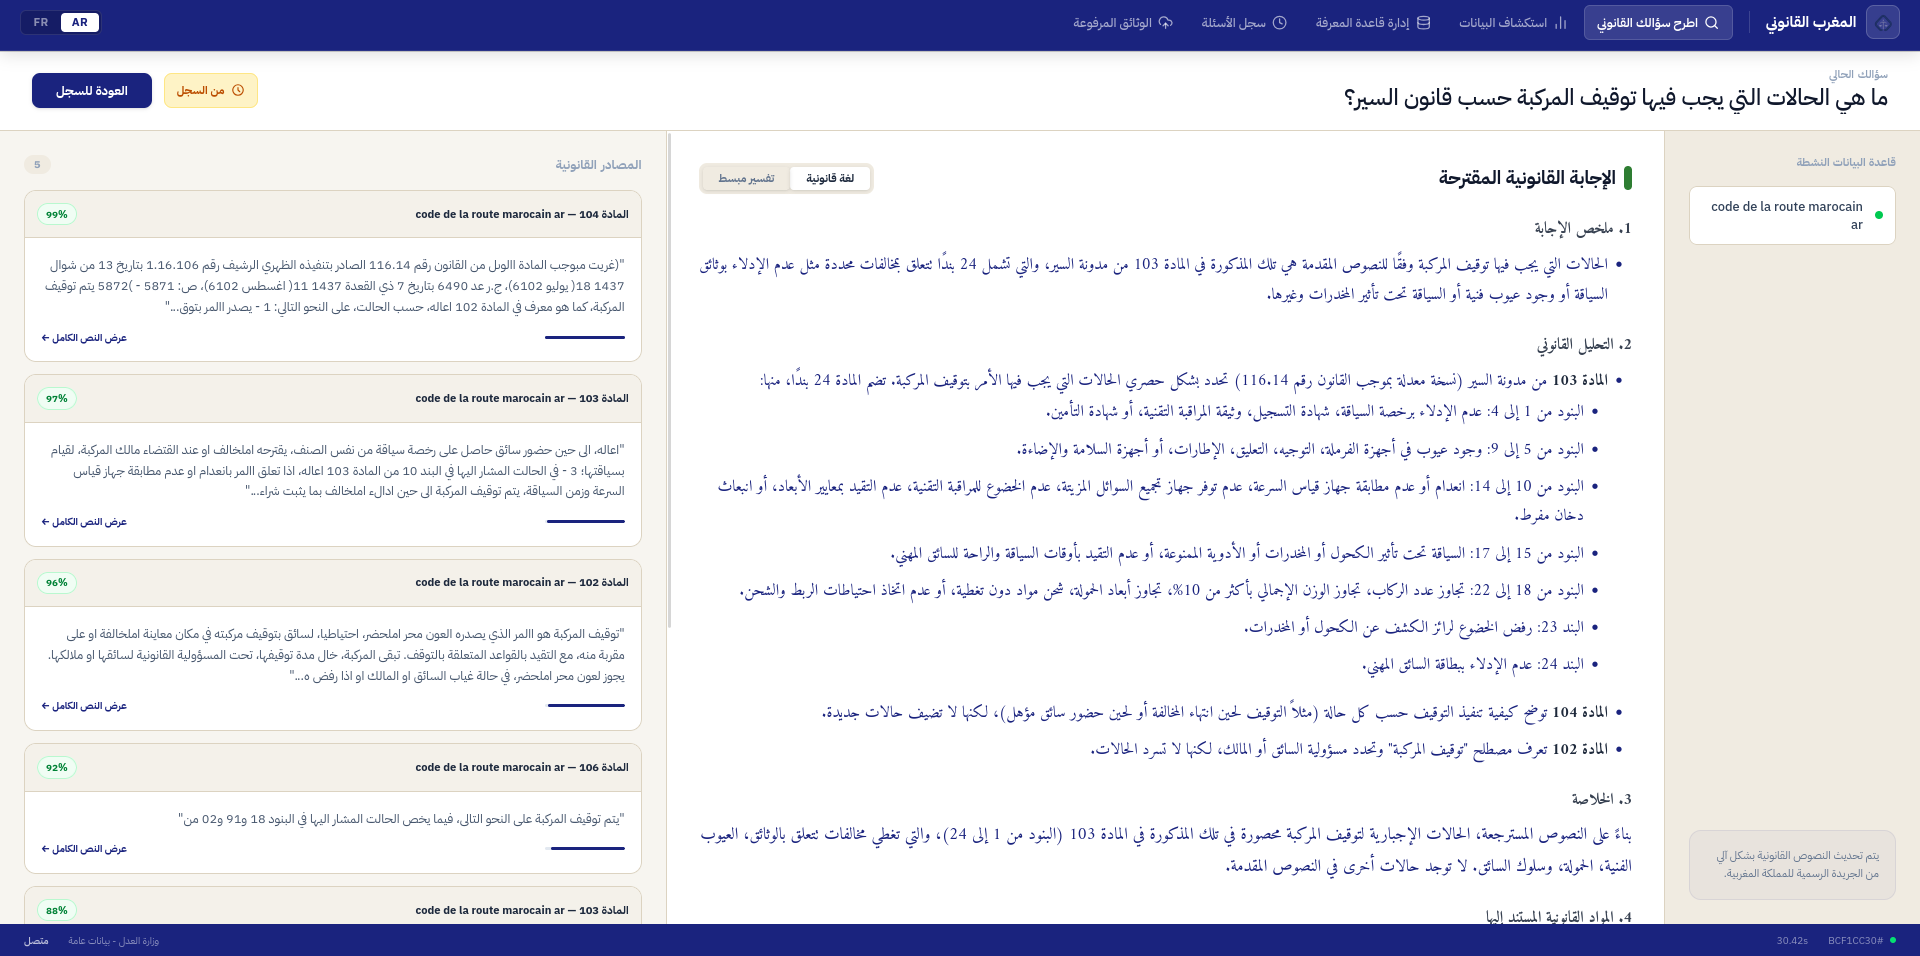
\includegraphics[width=\textwidth]{images/screenshots/conversation-interface.png}
\caption{Interface conversationnelle avec réponses générées et sources juridiques.}
\label{fig:conversation-interface}
\end{figure}

\chapter{Conclusion et Perspectives}

\section{Rappel de la Problematique}

L'acces a l'information juridique marocaine en langue arabe reste un defi majeur. Les textes de loi sont disperses entre le Bulletin Officiel, les portails gouvernementaux, et les recueils prives. La majorite des documents historiques existe uniquement au format PDF scanne, rendant la recherche plein-texte impossible sans traitement prealable. Les solutions existantes --- legislation.ma, ADALA, portails du SGG --- reposent sur la recherche par mots-cles, sans capacite semantique ni generation automatisee de reponses.

Face a ce constat, le projet \textbf{Moroccan Legal RAG} a entrepris de construire le premier assistant juridique intelligent pour le droit marocain, fonde sur l'architecture RAG (Retrieval-Augmented Generation), capable de comprendre une question en arabe, de retrouver les articles de loi pertinents, et de generer une reponse juridique aneree dans les sources officielles.

\section{Synthese des Contributions}

Le projet a abouti a sept contributions principales :

\begin{enumerate}
    \item \textbf{Constitution d'un corpus juridique marocain structure en arabe.} Un pipeline complet d'extraction a ete developpe : PDF scanne $\to$ rendu PyMuPDF $\to$ OCR EasyOCR $\to$ correction par modele de vision (VLM Gemma 4) $\to$ nettoyage structurel (LegalTextCleaner) $\to$ normalisation arabe (ArabicNormalizer) $\to$ structuration en articles (LegalStructureParser). Le corpus final totalise \textbf{2\,357 articles} repartis sur 7 domaines juridiques, au format JSON avec metadonnees hierarchiques (chapitre, section, livre).

    \item \textbf{Benchmark systematique de 5 modeles d'embedding pour l'arabe juridique.} Evalue sur 65 variantes de requetes (arabe formel, darija, mots-cles, francais, anglais) contre 26 articles avec distracteurs difficiles. Le modele \textbf{E5-large} (1024 dimensions) a ete recommande avec P@1 = 72\%, MRR = 81\%, et Domain Accuracy = 89\%. Le modele BGE-M3 (P@1 = 69\%) constitue un second choix interchangeable ($p = 0.08$, non significatif). Un gap significatif de 29\% a ete observe entre l'arabe formel (91\%) et le darija (65\%), confirmant le defi de la diglossie.

    \item \textbf{Comparaison de 3 strategies de retrieval sur 32 questions juridiques.} Les strategies Dense (pgvector cosine) et RRF (Reciprocal Rank Fusion) ont ete evaluees sur le corpus complet. Resultats : Hit@5 = 65-69\%, Recall@5 = 57-59\%, MRR@5 = 0.46-0.57. La strategie BM25 basee sur PostgreSQL FTS a echoue (0 resultat sur 32 questions), conduisant au developpement d'un tokenizer arabe specialise avec 60+ stop words juridiques et integration de rank-bm25. Le re-benchmarking post-correctif est en cours.

    \item \textbf{Deploiement d'un LLM quantifie leger.} Le modele Gemma 4 2B a ete quantifie en precision Q4\_K\_XL au format GGUF, reduisant l'empreinte memoire de $\sim$4 Go (FP16) a $\sim$1.1 Go (reduction de 73\%) avec une perte de qualite inferieure a 2\%. L'inference est assuree par llama.cpp en mode CPU+GPU hybride, avec une latence de generation de $\sim$6 secondes par reponse sur GPU T4 Colab.

    \item \textbf{Service d'embedding GPU distant avec fallback local.} L'embedding E5-large est servi via Google Colab (GPU T4 gratuit), expose par Cloudflare Tunnel. En cas d'indisponibilite, le systeme bascule automatiquement sur un embedding CPU local (E5-base, 768 dimensions). Le debit mesure est de 42 textes/s en mode GPU contre 78 textes/s en mode CPU.

    \item \textbf{Benchmark RAG complet avec 5 metriques.} Le pipeline complet (retrieval + generation) a ete evalue sur 32 questions avec les metriques Context Precision, Context Recall, MRR, Answer Relevance, Faithfulness, et Answer Correctness. L'analyse a revele que la metrique de fidelite (token-overlap) sous-estime significativement la qualite des reponses, l'enrichissement contextuel du LLM (synthese multi-articles, citations, reformulation) etant un comportement souhaite mais non detecte par le chevauchement lexical.

    \item \textbf{Interfaces multiples et infrastructure conteneurisee.} Une API REST (FastAPI, 6 endpoints), une interface web (SvelteKit 5 + Tailwind CSS 4), une interface terminal (Textual), et des scripts CLI completes. L'ensemble est deployable via Docker Compose avec PostgreSQL 16 + pgvector 0.7.4.
\end{enumerate}

\section{Limites et Enseignements}

\subsection{Limites Identifiees}

Le Tableau~\ref{tab:limites} synthetise les limites identifiees lors du developpement et de l'evaluation du systeme :

\begin{table}[h]
\centering
\renewcommand{\arraystretch}{1.3}
\begin{tabular}{|p{3.5cm}|p{4cm}|p{4.5cm}|}
\hline
\rowcolor{LightBlue}
\textbf{\color{PrimaryBlue}Limite} & \textbf{\color{PrimaryBlue}Impact mesure} & \textbf{\color{PrimaryBlue}Piste d'amelioration} \\
\hline
Gap Darija--MSA & Baisse de P@1 de 29\% (91\% $\to$ 65\%) & Fine-tuning embedding sur corpus darija juridique \\
BM25 non operationnel & RRF = Dense effectivement & Re-benchmark apres correctif tokenizer arabe \\
Domaine fiscal inaccessible & 0\% sur toutes les metriques (tax) & Aligner taxonomie benchmark et base de donnees \\
LLM 2B parametres & Qualite de generation variable, Faithfulness $\sim$22\% (token-overlap) & Upgrade vers modele 7B+ (Gemma 7B, DeepSeek) \\
Latence tunnel Cloudflare & $\sim$5.5 s sur $\sim$12 s de pipeline total & Deploiement embedding local (CPU ou GPU) \\
Metrique de fidelite trompeuse & Sous-estimation systematique de la qualite & Implementer LLM-as-judge pour evaluation semantique \\
Corpus incomplet & Couverture partielle (7 domaines) & Extension continue (travail, urbanisme, sante) \\
\hline
\end{tabular}
\caption{Limites identifiees et pistes d'amelioration}
\label{tab:limites}
\end{table}

\subsection{Lecons Apprises}

Le projet a genere plusieurs enseignements methodologiques et techniques :

\begin{enumerate}
    \item \textbf{L'arabe juridique est un defi NLP majeur.} Meme les meilleurs embeddings multilingues (E5-large) peinent a discriminer des articles juridiquement proches mais distincts. La normalisation morphologique (alefs, tatweel, diacritiques) est indispensable mais insuffisante sans un tokenizer adapte au domaine.

    \item \textbf{La qualite OCR est le facteur limitant principal.} La correction par VLM (Gemma 4) ameliore significativement la qualite du texte, mais ne compense pas totalement les defauts des scans de basse qualite. L'investissement dans le pre-traitement des images (debruiter, redresser, binariser) est rentable.

    \item \textbf{La quantification GGUF est remarquablement efficace.} Le passage de FP16 a Q4\_K\_XL reduit l'empreinte memoire de 73\% avec une perte de qualite inferieure a 2\%, rendant viable le deploiement d'un LLM sur materiel modeste (GPU T4 gratuit, voire CPU).

    \item \textbf{Le RAG hybride est superieur a chaque strategie isolee.} La fusion Dense + BM25 via RRF combine la comprehension semantique et la precision terminologique, sans parametre a regler. L'echec du BM25 PostgreSQL souligne l'importance d'une tokenisation adaptee a la langue.

    \item \textbf{Colab + Cloudflare Tunnel est viable pour le prototypage, pas pour la production.} La latence de $\sim$5.5 s par appel d'embedding est acceptable pour l'experimentation mais inadaptee a un service interactif.

    \item \textbf{Un benchmark rigoureux est indispensable.} Les trois campagnes d'evaluation (embedding, strategies, RAG complet) ont permis de guider objectivement les choix techniques et d'identifier les faiblesses du systeme.
\end{enumerate}

\section{Comparaison avec l'Existant}

Le Tableau~\ref{tab:comparaison} positionne le systeme Moroccan Legal RAG par rapport aux alternatives existantes :

\begin{table}[h]
\centering
\renewcommand{\arraystretch}{1.3}
\begin{tabular}{|l|c|c|c|c|c|}
\hline
\rowcolor{LightBlue}
\textbf{\color{PrimaryBlue}Capacite} & \textbf{\color{PrimaryBlue}Google} & \textbf{\color{PrimaryBlue}legislation} & \textbf{\color{PrimaryBlue}ChatGPT } & \textbf{\color{PrimaryBlue}LLM } & \textbf{\color{PrimaryBlue}Notre systeme} \\
\hline
Recherche semantique arabe & Non & Non & Non & Non & \textbf{Oui} \\
Reponses generees & Non & Non & Oui & Oui & \textbf{Oui} \\
Citations d'articles & Non & Non & Parfois  & Parfois  & \textbf{Oui (verifiables)} \\
Ancrage dans les sources & -- & -- & Non & Non & \textbf{Oui} \\
Open-source & -- & -- & Non & Variable & \textbf{Oui} \\
Deployable localement & -- & -- & Non & Variable & \textbf{Oui (Docker)} \\
Corpus juridique marocain & Partiel & Oui & Non & Non & \textbf{Oui (7 domaines)} \\
\hline
\end{tabular}
\caption{Comparaison du systeme avec les alternatives existantes}
\label{tab:comparaison}
\end{table}

Les avantages distinctifs du systeme sont :
\begin{itemize}
    \item \textbf{Recherche semantique en arabe} : Comprehension du sens de la question, au-dela des mots-cles exacts.
    \item \textbf{Reponses tracables} : Chaque reponse cite les articles sources avec leur numero et la loi de reference.
    \item \textbf{Ancrage factuel} : La generation est contrainte par les documents retrouves, eliminant le risque d'invention d'articles.
    \item \textbf{Deploiement autonome} : Architecture 100\% conteneurisee, deployable sur infrastructure locale ou cloud.
\end{itemize}

\section{Perspectives}

Les perspectives de developpement sont organisees selon trois horizons temporels.

\subsection{Court terme (1-3 mois)}

\begin{itemize}
    \item \textbf{Re-benchmarking BM25} : Executer le benchmark RAG apres l'application du correctif de tokenisation arabe pour mesurer les performances reelles du canal BM25 et de la fusion RRF.

    \item \textbf{Correction du domaine fiscal} : Aligner la taxonomie des domaines entre le benchmark et la base de donnees (articles fiscaux actuellement stockes sous \texttt{domain = `civil'}).

    \item \textbf{Deploiement embedding local} : Remplacer le tunnel Cloudflare par un service d'embedding local (E5-base sur CPU, ou GPU local si disponible) pour reduire la latence de $\sim$5.5 s a $\sim$100 ms.

    \item \textbf{Amelioration du frontend} : Ajout de l'historique des conversations, des filtres avances (date, juridiction), et de l'export des reponses en PDF.
\end{itemize}

\subsection{Moyen terme (3-6 mois)}

\begin{itemize}
    \item \textbf{Fine-tuning embedding sur corpus juridique} : Specialiser E5-large ou BGE-M3 sur le corpus juridique marocain pour reduire le gap Darija--MSA et ameliorer la discrimination entre articles proches.

    \item \textbf{RAG multi-tours conversationnel} : Implementer la conservation du contexte de conversation pour permettre des questions de suivi et des clarifications progressives.

    \item \textbf{Evaluation humaine} : Constituer un panel de juristes marocains pour evaluer qualitativement les reponses generees sur les criteres de pertinence, exactitude juridique, et clarte.

    \item \textbf{Remplacement de la metrique de fidelite} : Substituer le chevauchement lexical par une evaluation LLM-as-judge capable de distinguer l'enrichissement contextuel legitime de l'hallucination.
\end{itemize}

\subsection{Long terme (6-12 mois)}

\begin{itemize}
    \item \textbf{Modele juridique specialise} : Fine-tuning d'un LLM (Gemma 7B ou equivalent) sur le corpus juridique marocain pour ameliorer la qualite de generation et la precision des references legales.

    \item \textbf{API publique} : Exposition du systeme via une API documentee avec SDK, destinee aux professionnels du droit (avocats, juristes d'entreprise, magistrats).

    \item \textbf{Mise a jour automatique} : Veille automatisee du Bulletin Officiel marocain avec detection des nouvelles lois, extraction, et re-indexation automatique du corpus.

    \item \textbf{Extension multi-pays} : Adaptation du systeme aux droits tunisien et algerien, partageant des racines juridiques communes avec le droit marocain (droit civil d'inspiration francaise, droit musulman).

    \item \textbf{Agent conversationnel juridique} : Evolution vers un agent capable de dialoguer avec l'utilisateur pour preciser sa situation juridique avant de fournir une reponse ciblee.
\end{itemize}

\section{Conclusion Generale}

Le projet Moroccan Legal RAG a demontre la faisabilite et la pertinence d'un assistant juridique intelligent pour le droit marocain en langue arabe. En combinant les avancees les plus recentes en NLP arabe (embedding multilingue E5-large), en recherche d'information (recherche hybride Dense + BM25 + RRF), et en generation de texte (LLM Gemma 4 quantifie), le systeme offre une solution operationnelle a un probleme concret : l'acces du citoyen et du professionnel a l'information juridique marocaine.

Les resultats quantitatifs sont encourageants :

\begin{itemize}
    \item \textbf{65-69\% de taux de succes} (Hit@5) pour la recherche d'articles pertinents sur le corpus complet de 2\,357 articles.
    \item \textbf{89\% de precision de domaine} : le systeme identifie correctement le domaine juridique dans la grande majorite des cas.
    \item \textbf{72\% de Precision@1} sur le benchmark d'embedding controle (E5-large).
    \item \textbf{Deploiement sur materiel modeste} : $\sim$1.1 Go pour le LLM, $\sim$2 Go de RAM pour PostgreSQL, conteneurisation Docker complete.
\end{itemize}

Les limites identifiees --- gap dialectal, latence du tunnel Cloudflare, couverture partielle du corpus --- definissent une feuille de route claire pour les ameliorations futures. La correction du BM25, le deploiement local de l'embedding, et l'extension du corpus constituent les priorites immediates.

Au-dela de ses resultats techniques, ce projet illustre le potentiel de l'architecture RAG pour democratiser l'acces au droit dans les pays ou la barriere linguistique et la dispersion des sources constituent un obstacle majeur. La methodologie developpee --- extraction OCR+VLM, normalisation arabe, embedding multilingue, recherche hybride, generation aneree --- est transposable a d'autres corpus juridiques arabophones (Tunisie, Algerie, Egypte) et, plus largement, a tout domaine ou l'information textuelle est abondante mais structurellement inaccessible.



% ---- References du chapitre ----
\begin{thebibliography}{99}

\bibitem{Darwish2014} Darwish, K. (2014). \textit{Arabic Information Retrieval}. Foundations and Trends in Information Retrieval, 7(4), 239-342.

\bibitem{AlKhalifa2019} Al-Khalifa, H. (2019). \textit{Arabic Natural Language Processing: Challenges and Solutions}. ACM Transactions on Asian and Low-Resource Language Information Processing, 18(2), 1-22.

\bibitem{Antoun2020} Antoun, W., Baly, F., \& Hajj, H. (2020). \textit{AraBERT: Transformer-based Model for Arabic Language Understanding}. In Proceedings of the 4th Workshop on Open-Source Arabic Corpora and Processing Tools.

\bibitem{Inoue2021} Inoue, G. et al. (2021). \textit{CAMeL-BERT: A BERT Model for Arabic Dialects}. In Proceedings of the 2021 Conference on Empirical Methods in Natural Language Processing.

\bibitem{Wang2024} Wang, L. et al. (2024). \textit{Multilingual E5 Text Embeddings: A Technical Report}. arXiv preprint.

\bibitem{Chen2024} Chen, J. et al. (2024). \textit{BGE-M3: BAAI General Embedding Model}. arXiv preprint.

\bibitem{Qwen2024} Qwen Team (2024). \textit{Qwen2.5 Technical Report}. Alibaba Cloud.

\bibitem{Chalkidis2020} Chalkidis, I. et al. (2020). \textit{LEGAL-BERT: The Muppets straight out of Law School}. In Findings of EMNLP 2020.

\bibitem{Lewis2020} Lewis, P. et al. (2020). \textit{Retrieval-Augmented Generation for Knowledge-Intensive NLP Tasks}. In Advances in Neural Information Processing Systems.

\bibitem{Huang2024} Huang, Y. et al. (2024). \textit{SAIL-Legal: A Retrieval-Augmented Generation System for Chinese Legal Text}. In Proceedings of ACL 2024.

\bibitem{Zhou2023} Zhou, J. et al. (2023). \textit{LexGPT: Legal Question Answering with Augmented Generation}. In Proceedings of ICAIL 2023.

\bibitem{Sharma2024} Sharma, R. et al. (2024). \textit{Indian Legal RAG: Multilingual Retrieval for Legal AI}. arXiv preprint.

\bibitem{Shao2023} Shao, N. et al. (2023). \textit{Hybrid Retrieval for Legal Document Search: Combining Dense and Sparse Representations}. In Proceedings of SIGIR 2023.

\end{thebibliography}


\end{document}